\section{Theory overview}
\label{sec:theoryoverview}

In this section we summarize the theoretical background that underlies
lattice-QCD calculations of PDF-related quantities, on the one hand, and 
phenomenological fits of PDFs, on the other hand.
%
We first review the general framework in which unpolarized and 
polarized PDFs are defined, then we present the available lattice-QCD 
and global-fit approaches to determine them. 
%
The discussion is restricted to the information required to connect the
lattice-QCD and global-fit methods.
%
We have devoted particular attention to ensuring a unified and
consistent notation between the two.
%
An extended treatment of the subjects discussed in this section
can be found in dedicated reviews.
%
We refer the interested reader to Refs.~\cite{Olive:2016xmw,Gupta:1997nd}
for lattice QCD and to Refs.~\cite{Perez:2012um,DeRoeck:2011na,Alekhin:2011sk,
Ball:2012wy,Forte:2013wc,Jimenez-Delgado:2013sma,Rojo:2015acz,
Butterworth:2015oua,Accardi:2016ndt,Gao:2017yyd} for global fits.
%
Details on the framework underlying PDFs can be found in general 
textbooks~\cite{Ellis:1991qj,Leader:2001gr,Collins:2011zzd,
DeGrand:2006zz,Gattringer:2010zz}.

\subsection{Parton distribution functions}
\label{Sec:IntroPDFs}

Quantum chromodynamics is the non-abelian quantum field 
theory that describes the strong interaction.
%
It provides the theoretical foundation for the phenomenological ideas of 
quark model, color charge, and partons as hadron constituents.
%
The power of QCD to describe physics from the pion mass scale all the way up 
to the scale of high-energy colliders, such as the LHC, relies on the 
remarkable properties of asymptotic freedom~\cite{Gross:1973ju,Gross:1973id,
Gross:1974cs,Politzer:1974fr} and 
factorization~\cite{Collins:1987pm,Collins:1989gx}.

At high energies, or short distances, the QCD coupling is small 
and perturbation theory can accurately characterize the relevant scattering 
processes~\cite{Campbell:2006wx}.
%
At low energies, or larger distances, nonperturbative effects give rise to 
quark confinement and spontaneous chiral symmetry breaking~\cite{Gasser:1983yg}.
%
The connection between low- and high-energy dynamics is provided by QCD 
factorization theorems~\cite{Collins:1987pm,Collins:1989gx}: 
short-distance physics above the factorization scale $\mu$ is captured by 
partonic hard-scattering cross-sections calculated perturbatively as a 
power series expansion in the QCD coupling, while the 
long-distance physics below the factorization scale $\mu$ is described by 
nonperturbative quantities.
%
In a collinear, leading-twist factorization framework, these quantities are
universal ({\it i.e.} process-independent) PDFs.
%
Depending on the helicity state of the parent hadron, one usually 
distinguishes between helicity-averaged (unpolarized, henceforth)
and helicity-dependent (polarized, henceforth) PDFs.

Unpolarized PDFs are denoted as 
\begin{equation}
f(x,\mu^2)\equiv f^{\rightarrow}(x,\mu^2) + f^{\leftarrow}(x,\mu^2)\mbox{,}\qquad 
f=\{g,u,\bar{u},d,\bar{d},s,\bar{s},...\}
\,\mbox{,}
\label{eq:unpPDFs}
\end{equation}
where $x$ is the fraction
of the hadron longitudinal momentum carried by the parton,
and the sum over parton's helicities aligned along ($\rightarrow$) and 
opposite ($\leftarrow$) the parent's nucleon helicity is made explicit.
%
An additional index could be used to denote the hadronic species (proton,
neutron, pion, \dots).
%
However, we omit such a designation, as we only refer to the proton
in this paper.

At leading order (LO) in the QCD coupling series, unpolarized PDFs 
describe the probability distribution of a parton with a specified 
momentum fraction $x$.
%
The total momentum carried by each parton flavor is then given by 
the first moment of the corresponding PDF, for instance
%
\begin{align}
\int_{0}^{1}dx\ x\ \left[u(x,\mu^2)\right] 
= & {}  
\left\langle x\right\rangle _{u}(\mu^2)\,, \label{eq:umoment1}\\
\int_{0}^{1}dx\ x\ \left[u(x,\mu^2)+\bar{u}(x,\mu^2)\right] 
= & {} 
\left\langle x\right\rangle _{u^{+}}(\mu^2)\,. \label{eq:uplusmoment1}
\end{align}
%
Here, $\left\langle x\right\rangle _{u}$ is the momentum
carried by the up-quark, and $\left\langle x\right\rangle _{u^{+}}$ is
the momentum carried by the sum of up and anti-up quarks~\footnote{We always 
 refer to $q^+$ to indicate the sum of the quark and anti-quark PDFs of the 
 same flavor.},
see Appendix~\ref{app:notation} for our notational conventions.

Polarized PDFs describe the extent to which quarks and gluons 
with a given momentum fraction $x$ have their spins aligned with the spin 
direction of a fast moving nucleon in a helicity eigenstate. 
%
They are denoted as 
\begin{equation}
\Delta f(x,\mu^2) \equiv f^{\rightarrow}(x,\mu^2) - f^{\leftarrow}(x,\mu^2)
\mbox{,}\qquad f=\{g,u,\bar{u},d,\bar{d},s,\bar{s},...\}
\,\mbox{,}
\label{eq:polPDFs}
\end{equation}
where, as in Eq.~\eqref{eq:unpPDFs}, $x$ is the fractional 
momentum carried by the parton,
and the parton's spin alignment along ($\rightarrow$) or opposite 
($\leftarrow$) the polarization direction of its parent nucleon
is made explicit.

Much of the interest in polarized PDFs is related to the fact that 
their zeroth moments can be interpreted as the fractions of the proton's 
spin carried by the corresponding partons.
%
They are therefore the key to one of the most fundamental, 
but not yet satisfactorily answered questions in hadronic physics,
{\it i.e.}, how the spin of the proton is distributed among its constituents.
%
Specifically, the zeroth moments of the singlet and the gluon polarized PDFs,
\begin{align}
\Delta\Sigma(\mu^2)
& =
\sum_{q}^{N_f}\int_0^1 dx 
\left[\Delta q(x, \mu^2) + \Delta\bar{q}(x, \mu^2)\right]
\equiv
\sum_q^{N_f}\langle 1 \rangle_{\Delta q^+}(\mu^2)\,,
\label{eq:singletmom}
\\
\Delta G(\mu^2)
& =
\int_0^1 dx \Delta g(x,\mu^2)
\equiv
\langle 1 \rangle_{\Delta g}(\mu^2)
\,,
\label{eq:moments}
\end{align}
where $N_f$ is the number of active flavors,
directly contribute to the proton spin sum rule~\cite{Leader:2013jra}.

Beyond LO, PDFs are renormalization scheme-dependent 
quantities, typically worked out in the $\overline{\rm MS}$ 
scheme~\cite{tHooft:1973mfk,Weinberg:1951ss}.
%
When PDFs are convolved with the appropriate partonic hard-scattering 
cross-sections, computed in the same scheme, the corresponding physical 
observables are scheme-independent, up to subleading spurious 
terms in the perturbative expansion. 

Both unpolarized and polarized PDFs are accessible, theoretically and 
experimentally, through the forward Compton scattering amplitude
\begin{equation}
\label{eq:Compton}
T_{\mu\nu}(p,q,s) 
= 
\int {\rm d}^4\!z\, e^{iqz}  \langle p,s |T J_\mu(z) J_\nu(0)|p,s\rangle
\end{equation}
at large virtual photon momenta $q^2=-Q^2$. 
%
Here $T$ is the time-ordering operator, $J_\mu(z)$ and $J_\nu(0)$ are vector
currents at space-time points $z$ and $0$ respectively, and the 
external states are hadronic states with momentum $p$ and spin $s$.

The most general form of the Compton amplitude $T_{\mu\nu}(p,q)$ 
reads~\cite{Manohar:1992tz}
\begin{align}
T_{\mu\nu}(p,q,s) 
= {} & 
  \left(-g_{\mu\nu}+\frac{q_\mu q_\nu}{q^2}\right)\mathcal{F}_1(\omega,Q^2) 
+ \left(p_\mu-\frac{p\cdot q}{q^2}q_\mu\right) \left(p_\nu-\frac{p\cdot q}{q^2}q_\nu\right) \frac{1}{p\cdot q} \mathcal{F}_2(\omega,Q^2)
\nonumber\\ 
& {} \quad  
+ i\,\epsilon_{\mu\nu\lambda\sigma}q^\lambda s^\sigma \frac{1}{p\cdot q}\mathcal{G}_1(\omega,Q^2)
+ i\,\epsilon_{\mu\nu\lambda\sigma}q^\lambda \left(p\cdot q\, s^\sigma - s\cdot q\, p^\sigma\right) \frac{1}{(p\cdot q)^2}\mathcal{G}_2(\omega,Q^2)\,,
\label{eq:Comptampl}
\end{align}
where $\omega=2p\cdot q/q^2$ and $\mathcal{F}_1$, $\mathcal{F}_2$, 
$\mathcal{G}_1$ and $\mathcal{G}_2$ are the Compton amplitude structure 
functions.
%
They can be related to the electromagnetic structure functions
$F_1$, $F_2$, $g_1$ and $g_2$, used to parametrize the deep-inelastic 
scattering (DIS) hadronic tensor\footnote{A more
 general expression of the DIS hadronic tensor including electroweak currents
 can be worked out, see~\cite{Anselmino:1993tc,Anselmino:1992rn}.}
\begin{align}
W_{\mu\nu}(p,q,s)
= {} &
\frac{1}{4\pi}\int d^4z e^{iqz}\langle p,s |[J_\mu(z),J_\nu(0)]|p,s\rangle
\nonumber
\\
= {} &
\left(-g_{\mu\nu} +  \frac{q_\mu q_\nu}{q^2}\right) F_1(x,Q^2)
+\left( p_\mu - \frac{p\cdot q}{q^2}q_\mu \right)
 \left(p_\nu - \frac{p\cdot q}{q^2}q_\nu \right) \frac{1}{p\cdot q}
F_2(x, Q^2)
\nonumber
\\
& +i\,\epsilon_{\mu\nu\lambda\sigma}q^\lambda s^\sigma
\frac{1}{p\cdot q} g_1(x,Q^2)
+ i\,\epsilon_{\mu\nu\lambda\sigma}q^\lambda(p\cdot q\, s^\sigma - s\cdot q\, p^\sigma)
\frac{1}{(p\cdot q)^2}g_2(x,Q^2)\,,
\label{eq:hadtensor}
\end{align}
where $x=1/\omega$ is the Bjorken variable identified with the parton
fractional momentum at Born level; 
see~\cite{Anselmino:1992rn,Manohar:1992tz} for details.
%
Specifically, given the definitions in \eqref{eq:Comptampl} and 
\eqref{eq:hadtensor}, the optical theorem implies that twice the imaginary 
part of $T_{\mu\nu}$ is equal to $W_{\mu\nu}$ times $4\pi$.
%
Neglecting target mass corrections, one has
\begin{align}
\mathcal{F}_1(\omega,Q^2) 
= {} & 2 \omega^2 \int_0^1 dx\,  \frac{xF_1(x,Q^2)}{1-(\omega x)^2} 
= \sum_{n=2,4,\cdots}^\infty 2\omega^n \int_0^1 dx\, x^{n-1} F_1(x,Q^2) \,, \\
\mathcal{G}_1(\omega,Q^2) 
= {} & 2 \omega \int_0^1 dx\, \frac{g_1(x,Q^2)}{1-(\omega x)^2} 
= \sum_{n=1,3,\cdots}^\infty 2\omega^n \int_0^1 dx\, x^{n-1} g_1(x,Q^2)\,.
\end{align}

At a sufficiently high momentum transfer $Q^2$, power corrections can be 
neglected and QCD factorization allows one to write the structure functions 
$F_1(x,Q^2)$ and $g_1(x,Q^2)$ as a convolution between perturbatively-computable
hard-scattering cross-sections and nonperturbative parton distributions:
\begin{align}
F_1(x,Q^2) 
= {} 
& x\sum_f \int_x^1 \frac{{\rm d}z}{z}\,C_{1,f}\left(\frac{x}{z},\alpha_s(Q^2)\right)f(z,Q^2) \,, \label{eq:Fi}\\
g_1(x,Q^2) 
= {} 
& \sum_f \int_x^1\frac{dz}{z}\, \Delta C_{1,f}\left(\frac{x}{z},\alpha_s(Q^2)\right) \Delta f(z,Q^2) \,.
\label{pdf}
\end{align}
%
Here, the sums run over the number of active
flavors at the scale $Q^2$ (including the gluon), $C_{1,f}$ and 
$\Delta C_{1,f}$ are the perturbative partonic hard-scattering cross-sections,
$\alpha_s$ is the QCD strong coupling, and $f(x,Q^2)$ and $\Delta f(x,Q^2)$ 
are the unpolarized and polarized PDFs.

Parton distributions allow for a proper field-theoretic definition as matrix 
elements in a hadron state of bilocal operators that act to count the number 
of quarks and gluons carrying a fraction $x$ of the hadron's momentum.
%
The definitions are usually stated in the light-cone frame, where 
the hadron carries momentum $p$ with plus/minus components
$p^\pm=(p^0\pm p^3)/\sqrt{2}$, and transverse components equal to zero.
%
For example, in the case of unpolarized and polarized quark PDFs, one has
\begin{align}
q(x) & = \frac{1}{4\pi}
\int dy^-e^{-iy^-xp^+}\langle p|\bar{\psi}(0,y^-,\mathbf{0}_\perp)
\gamma^+\mathcal{G}\psi(0,0,\mathbf{0})|p\rangle\,,
\label{eq:LCdefunp}\\
\Delta q(x) & = \frac{1}{4\pi}
\int dy^-e^{-iy^-xp^+}\langle p, s|\bar{\psi}(0,y^-,\mathbf{0}_\perp)
\gamma^+\gamma^5\mathcal{G}\psi(0,0,\mathbf{0})|p, s\rangle\,,
\label{eq:LCdefpol}
\end{align}
where $\psi$ is the quark field and $\mathcal{G}$ is an appropriate gauge link
required to make Eqs.~\eqref{eq:LCdefunp}--\eqref{eq:LCdefpol} gauge invariant.
%
See Refs.~\cite{Collins:1981uw,Curci:1980uw,Baulieu:1979mr,Collins:1989gx} 
for the definition of $\mathcal{G}$ and for
explicit light-cone formul{\ae} of unpolarized an polarized gluon PDFs.

While PDFs cannot be calculated perturbatively, their dependence on the scale 
$\mu$ resulting from factorization can be.
%
This is done by means of the
DGLAP (Dokshitzer-Gribov-Lipatov-Altarelli-Parisi) 
evolution equations~\cite{Dokshitzer:1977sg,Gribov:1972ri,Altarelli:1977zs},
a set of integro-differential coupled equations of the form
\begin{equation}
  \label{eq:dglapunp}
\frac{\partial f^\prime(x,\mu^2)}{\partial \ln \mu^2}
=
\sum_{f=g,q,\bar{q}}\int_x^1 
\frac{{\rm d}z}{z}P_{f^\prime f}\left(\frac{x}{z},\alpha_s(\mu^2)\right)f(z,\mu^2)\, ,
\end{equation}
%
\begin{equation}
  \label{eq:dglappol}
\frac{\partial \Delta f^\prime(x,\mu^2)}{\partial \ln \mu^2}
=
\sum_{f=g,q,\bar{q}}\int_x^1 
\frac{{\rm d}z}{z}\Delta P_{f^\prime f}\left(\frac{x}{z},\alpha_s(\mu^2)\right)\Delta f(z,\mu^2)\, .
\end{equation}
%
In short, the logarithmic derivative of the PDF is determined by a convolution
of the PDFs with the unpolarized (polarized) DGLAP kernels $P_{f^\prime f}$
($\Delta P_{f^\prime f}$), which can be 
computed perturbatively in powers of $\alpha_{s}$.
%
The unpolarized splitting functions $P_{f^\prime f}$ are currently completely 
known up to NNLO~\cite{Moch:2004pa,Vogt:2004mw} in the $\overline{\rm MS}$ 
renormalization scheme.
%
Results for the unpolarized nonsinglet splitting functions have appeared 
recently at N$^3$LO~\cite{Davies:2016jie,Moch:2017uml}.
%
The polarized splitting functions $\Delta P_{f^\prime f}$ are currently known 
up to  NNLO~\cite{Moch:2014sna} in the $\overline{\rm MS}$ scheme.
%
The DGLAP evolution equations can be solved numerically using
either $x$-space or Mellin $N$-space techniques that are widely available 
in various public codes~\cite{Vogt:2004ns,Salam:2008qg,Botje:2010ay,
Bertone:2013vaa,Bertone:2015cwa}.
%
The typical level of agreement for the results of the PDF evolution 
has been demonstrated to be of 
$\mathcal{O}(10^{-5})$~\cite{Giele:2002hx,Dittmar:2005ed}.

%The power series expansion of both the unpolarized and polarized 
%splitting functions contains terms proportional to $\ln\mu^2$, 
%$\ln(1/x)$ and $\ln(1-x)$.
%
%While DGLAP evolution sums power of $\alpha_s\ln\mu^2$ contributions,
%in the small-$x$ kinematic region one may also sum power of $\ln(1/x)$
%contributions, independent of the value of $\mu^2$.
%
%This is achieved by the BFKL (Balitsky-Fadin-Kuraev-Lipatov) equations,
%which resum $\ln(1/x)$ terms to all orders.
%
%They were originally formulated in the unpolarized case at leading logarithm 
%(LL) order~\cite{Fadin:1975cb,Kuraev:1976ge,Kuraev:1977fs,Balitsky:1978ic},
%and later extended to next-to-leading logarithmic (NLL) 
%order~\cite{Fadin:1998py,Camici:1997ij,Ciafaloni:1998gs}
%
%The DGLAP and BFKL frameworks can be matched into a single set of evolution 
%equations by means of the small-$x$ resummation
%formalism~\cite{Ciafaloni:1999yw,Ciafaloni:2000cb,Ciafaloni:2003ek,
%Ciafaloni:2003rd,Altarelli:2005ni,White:2006yh,Altarelli:2008aj,
%Ciafaloni:2007gf,Bonvini:2016wki}.

%In the polarized case, the use of the small-$x$ formalism was pioneered 
%decades ago by Kirschner and Lipatov~\cite{Kirschner:1983di} 
%(see also~\cite{Kirschner:1994rq,Kirschner:1994vc,Griffiths:1999dj}) 
%and later by Bartels, Ermolaev, and Ryskin in the context of the structure 
%function $g_1$~\cite{Bartels:1995iu,Bartels:1996wc}.
%
%Small-$x$ evolution equations which resum powers of $\alpha_s\ln^2(1/x)$ 
%in the polarization-dependent evolution along with powers of $\alpha_s\ln(1/x)$
%in the unpolarized evolution have been recently reconsidered using the 
%formalism of Wilson line-like operators~\cite{Kovchegov:2015pbl}.
%
%Both numerical~\cite{Kovchegov:2016weo}
%and analytical~\cite{Kovchegov:2016zex,Kovchegov:2017jxc}
%solutions to these small-$x$ evolution equations have been derived
%for the flavor singlet combination of polarized PDFs.
%
%Results have been extended also to the case of the polarized gluon 
%PDF~\cite{Kovchegov:2017lsr}.


\subsection{Lattice QCD}
\label{Sec:IntroLQCD}

The lattice-QCD method is based on regularizing QCD on a finite Euclidean 
lattice and is generally studied by numerical computation of QCD correlation 
functions in the path-integral formalism~\cite{DiPierro:2000nt,Lepage:1998dt,
Luscher:1998pe,Gupta:1997nd}, using methods adapted from statistical 
mechanics~\cite{Binder:2015klx,Newman:1999mng}.
%
To make contact with experimental data, the numerical results are extrapolated 
to the continuum and infinite-volume limits.
%
The past decade has seen significant progress in the development of efficient 
algorithms for the generation of ensembles of gauge field configurations and 
tools for extracting the relevant information from lattice-QCD
correlation functions.
%
In this respect, lattice-QCD calculations have reached a level where
they not only complement, but also guide current and forthcoming
experimental programs~\cite{Brodsky:2015aia,Aschenauer:2014twa}.

In this section, we discuss the sources of systematic uncertainties
that affect current lattice QCD calculations, and we present 
lattice-QCD methods to determine either the Mellin moments of PDFs
or the complete PDF $x$-dependence.

\subsubsection{Systematic uncertainties}
Lattice-QCD calculations must demonstrate control over all sources of
systematic uncertainty introduced by the discretization of QCD on the
lattice to make meaningful contact with experimental data.
%
These
include discretization effects that vanish in the continuum limit;
extrapolation from unphysically heavy pion masses; finite volume
effects; and renormalization of composite operators.
%
To take the continuum limit requires accurate determinations of the 
lattice spacing.
% 
We briefly review these main sources of systematic uncertainty here; for a 
fuller account see, for example, Ref.~\cite{Aoki:2016frl}.

\begin{itemize}

\item {\bfseries Discretization effects and the continuum limit.} 
There is a fair degree of flexibility in discretizing the QCD action. 
%
This has led to a variety of formulations, which differ mainly in the choice of
the action for quarks.
%
In the continuum limit, which corresponds to taking
the lattice spacing $a$ to zero with all physical quantities fixed,
the simplest discretizations differ from continuum QCD at ${\mathcal
O}(a)$.
%
In practice, one cannot afford to perform numerical
simulations at arbitrarily small lattice spacings, because the cost of
computation increases with a large inverse power of the lattice
spacing, and ${\cal O}(a)$ effects can be significant even
with current lattice spacings ranging from $0.15 \,\mbox{fm}$ to
$0.05 \,\mbox{fm}$.
%
To accelerate the convergence to the continuum
limit, improved quark and gluon actions are widely used, which include
higher-dimension operators to reduce the discretization errors to
${\cal O}(a^2)$ or better.
%
Chiral fermions with automatic $\mathcal{O}(a)$ improvement and small 
$\mathcal{O}(a^2)$ discretization errors are also adopted to admit 
calculations on coarser lattice spacings~\cite{Creutz:2011hy,Vladikas:2011bp,
Chandrasekharan:2004cn}. 

\item {\bfseries Pion mass dependence.} 
The computational cost of the fermion contribution to the path
integral increases with a large inverse power of the bare quark mass
(or, equivalently, the pion mass).
%
Lattice-QCD calculations are therefore
often performed at unphysically heavy pion masses, although results calculated
directly with physical pion masses have become increasingly common, albeit with larger
errors.
%
To obtain results at the physical pion mass, lattice data are
generated at a sequence of pion masses and then extrapolated to the
physical pion mass.
%
To control the associated systematic
uncertainties, these extrapolations are guided by effective
theories.
%
In particular, the pion-mass dependence can be parametrized
using chiral perturbation theory ($\chi$PT)~\cite{Golterman:2009kw}, 
which accounts for the
Nambu-Goldstone nature of the lowest excitations that occur in the
presence of light quarks. 
%
%With multiple lattices at different sea quark masses including some
%at physical pion mass, several lattice spacings and volumes, one can  
%perform global fits with judicious functional forms to determine
%the final result at the physical pion mass and extrapolated continuum and 
%infinite volumes.

\item {\bfseries Finite volume effects.} Numerical lattice-QCD 
calculations are necessarily restricted to a finite space-time
volume, {\it e.g.}, a hypercube of side $L$.
%
For most simple quantities, these effects decay exponentially
with the size of the lattice~\cite{Luscher:1985dn,Luscher:1986pf}, and 
therefore the easiest way to
minimize or eliminate finite volume effects is to choose the volume
sufficiently large in physical units.
%
Unfortunately, this can be
prohibitively expensive as one approaches the continuum limit, requiring the
number of lattice sites to grow as $L/a$ in all four directions. 
%
Finite volume $\chi$PT is the preferred
tool to develop systematic expansions that provide quantitative
information on finite-volume effects.
%
In general, finite volume
effects of hadrons are dominated by their interactions with pions,
which can travel around the (periodic) lattice many times.
%
Numerical evidence suggests that lattice sizes of $m_\pi L \geq 4$, where
$m_\pi$ is the pion mass, are generally sufficiently large that finite
volume effects are negligible for mesons, within the current precision 
of lattice-QCD calculations.
%
From the studies of the pseudoscalar and electromagnetic form factors of the 
nucleon, it is evident that larger physical volumes are needed for the 
baryons.

\item {\bfseries Excited state contamination.} 
At small Euclidean times, a lattice-QCD correlation function
is a sum over a tower of states that behave as $e^{-m_it}$, where $m_i$ is the 
energy of the state and $t$ is the Euclidean time. 
%
Thus, at large Euclidean times,
ground-state quantities can be extracted by fitting to the dominant 
exponential behaviour.
%
Unfortunately, the signal-to-noise ratio is exponentially suppressed 
as $e^{-(E_N-3m_\pi/2)t}$, where $E_N$ is the nucleon energy~\cite{Lepage:1989hd}.
%
Thus, lattice-QCD results
are extracted from an intermediate region in which excited state contributions 
are either small or well-controlled and the signal-to-noise ratio is 
sufficiently large that the signal can be reliably extracted. 
%
This is a particular challenge for baryons and is one of the largest 
sources of systematic uncertainties for nucleon matrix elements.

\item {\bfseries Renormalization.} The matrix elements extracted from a 
lattice-QCD calculation at a given lattice spacing are bare matrix elements,
rendered finite by the presence of the lattice spacing, which serves
as a gauge-invariant UV regulator. 
%
To take the continuum limit, {\it i.e.}, remove the regulator, one must 
renormalize the corresponding operators and fields and match them to some 
common scheme and scale used by phenomenologists. 
%
Although renormalization is traditionally
discussed in the framework of perturbation theory, at hadronic energy
scales the renormalization constants should be computed
nonperturbatively to avoid uncontrolled uncertainties due to 
truncated perturbative results.
%
To compare with phenomenology, which uses the $\overline{\rm MS}$ scheme, 
a conversion factor from the nonperturbative scheme must be computed 
perturbatively. 
%
This requires a renormalization condition that can be implemented on the 
lattice and in continuum perturbation theory. 
%
In QCD with only light quarks it is technically advantageous to employ 
so-called mass-independent renormalization schemes. 
%
A common choice is the regularization-independent/momentum (RI/MOM) 
scheme~\cite{Martinelli:1994ty}.

In addition, on a hypercubic lattice, the orthogonal group $O(4)$ of
continuum Euclidean space-time is reduced to the hypercubic group
$H(4)$.
%
Thus, operators are classified according to irreducible
representations of $H(4)$~\cite{Gockeler:1996mu}.
%
Different irreducible representations belonging to the same $O(4)$ multiplet
will, in general, give different answers at finite lattice spacing, an effect 
that can be reduced by improving the operators~\cite{Gockeler:2004wp}.
%
Conversely, operators that lie in different irreducible representations of 
$O(4)$, but the same irreducible representations of $H(4)$, will mix at finite 
lattice spacing but not in the continuum. 
%
When these operators have lower mass dimensions,
the mixing coefficients scale with the inverse lattice spacing to some
power, and diverge in the continuum limit.
%
This power-divergent mixing
must be removed nonperturbatively, and is a particular challenge for
lattice calculations of the Mellin moments of PDFs (see
Sect.~\ref{Sec:MomentsLQCD}).

%Finally, it is worth noting that factorization, the key assumption of
%the operator product expansion (OPE), demands that the nonperturbatively 
%renormalized hadron matrix elements are matched to the perturbatively 
%renormalized Wilson coefficients at a scale where the perturbative 
%expressions show convergence. This appears to be
%the case for scales $\mu^2 \gtrsim 10\mbox{ GeV}^2$ at
%least~\cite{Gockeler:2010yr}. This, however, is a fundamental aspect
%of QCD, and is not restricted to lattice QCD. The DGLAP evolution equations,
%for example, work best for $q^2_{\rm min} \approx
%15\mbox{ GeV}^2$~\cite{Abramowicz:2015mha}, which should be kept in
%mind when comparing lattice results with phenomenology.

\item {\bfseries Lattice-spacing determination.} 
Numerical lattice-QCD calculations naturally determine all dimensionful 
quantities in units of the lattice spacing. 
%
Thus, extracting physical values requires the determination of the lattice 
scale. 
%
This is achieved by matching a quantity with mass dimension to its experimental 
value or through a well-defined theoretical procedure, that is referred to as
{\it scale-setting}. 
%
Popular reference scales include light decay constants, hadron masses, 
scales defined in terms of the heavy quark potential or, most recently, 
the length scales $\sqrt{t_0}$~\cite{Luscher:2010iy} and 
$w_0$~\cite{Borsanyi:2012zs} defined via the Wilson  gradient 
flow~\cite{Luscher:2010iy}. 
%
These scales can be computed cheaply and can be used to 
match scales between different gauge ensembles very accurately.  
%
However, a hadron mass or a decay constant -- which are known accurately 
from experiment and can be computed precisely in lattice-QCD -- 
have to be used for absolute scale setting. 
%
A popular hadronic mass for this purpose is the mass of the triply strange 
$\Omega$ baryon~\cite{Durr:2008zz} or the 2S-1S splitting in the Upsilon 
spectrum~\cite{Kendall:2008zz}.

\end{itemize}

These sources of systematic uncertainty all need to be under control
when confronting experimental data with lattice results, or vice
versa.
%
For a coherent assessment of the present state of lattice-QCD
calculations of various quantities, the degree to which each
systematic has been controlled in a given calculation is an important
consideration.
%
In Sect.~\ref{subsubsec:BClQCD}, we characterize the
quality of the lattice calculations, based on criteria inspired by the
FLAG analysis of flavor physics on the lattice~\cite{Aoki:2016frl}.

\subsubsection{Mellin moments of PDFs from lattice QCD}
\label{Sec:MomentsLQCD}

Parton distributions cannot be directly determined in Euclidean lattice QCD, 
because their field-theoretic definition involves fields at light-like 
separations.
%
Instead, the traditional approach for lattice-QCD calculations has been to 
determine the matrix elements of local twist-two operators, where twist is the 
dimension minus the spin, that can be related to the Mellin moments of PDFs.
%
In principle, given a sufficient number of Mellin moments, PDFs can be 
reconstructed from the inverse Mellin transform. In practice, however, 
the calculation is limited to the lowest three moments, because power-divergent 
mixing occurs between twist-two operators on the lattice.
%
Three moments are insufficient to fully reconstruct the momentum dependence of 
the PDFs without significant model dependence~\cite{Detmold:2003rq}.
%
The lowest three moments do provide, however, useful information, both as 
benchmarks of lattice-QCD calculations and as constraints in global extractions 
of PDFs. 
%
Here we briefly review the determination of Mellin moments of PDFs from lattice 
QCD. 

Using the Operator Product Expansion (OPE)~\cite{Zimmermann:1972tv}, the Mellin 
moments of the structure functions and the corresponding PDFs can be expressed, 
up to higher-twist effects, in terms of matrix elements of local operators:
\begin{align}
\!\!\!2 \int_0^1 dx\, x^{n-1} F_1(x,Q^2) &= \sum_a C_{1,a}^n(\mu^2)\, v_a^n(\mu^2)|_{\mu^2=Q^2} = \sum_a C_{1,a}^n(Q^2)\, \int_0^1 dx\, x^{n-1} f_a(x,Q^2)\,,\\
4 \int_0^1 dx\, x^n g_1(x,Q^2) &= \sum_a \Delta C_{1,a}^n(\mu^2)\, a_a^n(\mu^2)|_{\mu^2=Q^2} = \sum_a \Delta C_{1,a}^n(Q^2)\, \int_0^1 dx\, x^n\, 2 \Delta f_a(x,Q^2)\,,
\end{align}
where $v_i^n(\mu^2)$ and $a_i^n(\mu^2)$ are reduced matrix elements of the appropriate twist-two operators~\cite{Gockeler:1995wg},
\begin{align}
\frac{1}{2} \sum_s \langle p,s|\mathcal{O}^i_{\{\mu_1,\cdots,\mu_n\}}|p,s\rangle = {} & 2 v_i^n\, [p_{\mu_1}\cdots p_{\mu_n} - {\rm traces}] \,, \label{eq:twist2me}\\
\langle p,s|\mathcal{O}^{5\,i}_{\{\sigma \mu_1,\cdots,\mu_n\}}|p,s\rangle = {} & \frac{1}{n+1} a_i^n\, [s_\sigma p_{\mu_1}\cdots p_{\mu_n} - {\rm traces}]\,,
\end{align}
and $C_{1,i}^n(\mu^2)$ and $\Delta C_{1,i}^n(\mu^2)$ are the Mellin moments of the corresponding Wilson coefficients
\begin{equation}
C_{1,i}^n(\mu^2) = \int_0^1 dy\, y^{n-1} C_{1,i}(y,\mu^2)\,, \quad
\Delta C_{1,i}^n(\mu^2) = \int_0^1 dy\, y^n \Delta C_{1,i}(y,\mu^2)\,.
\end{equation}
The trace terms include operators with at least one factor of the metric 
tensor $g^{\mu_i \mu_j}$ multiplied by operators of dimension $(n+2)$ with 
$n-2$ Lorentz indices. 
%
The operators relevant for the lowest two moments are listed in 
Table~\ref{Tab:twist2}. 
%
The operator $\mathcal{O}^q_{\mu_1\mu_2}$ decomposes into two different 
representations of $H(4)$~\cite{Gockeler:1996mu}, each with different 
lattice artifacts and renormalization factors. 
%
In the continuum limit, however, both operators should lead to the same result. 
%
In contrast, the operator $\mathcal{O}^q_{\mu_1\mu_2\mu_3}$ splits into several 
representations of $O(4)$ transforming identically under $H(4)$ and causing 
the corresponding operators to mix under renormalization on the lattice.

%-------------------------------------------------------------------------------
\begin{table}
\renewcommand{\arraystretch}{1.6} 
\centering
\begin{tabular}{@{}ccc@{}}
\toprule
Matrix element & Operator & PDF moment \\ 
\midrule
$v_q^2$\,, $v_{\bar{q}}^2$  & 
$\displaystyle \left({\rm i}/2\right) \bar{q}(x)\gamma_{\mu_1} \overleftrightarrow{D}_{\mu_2} q(x)$ & 
$\langle x \rangle_{q^+}$\\
$v_q^3$\,, $v_{\bar{q}}^3$  & $\displaystyle \left({\rm i}/2\right)^2 \bar{q}(x)\gamma_{\mu_1} \overleftrightarrow{D}_{\mu_2} \overleftrightarrow{D}_{\mu_3} q(x)$ & $\langle x^2 \rangle_{q^-}$\\
$a_q^0$ & $\displaystyle \bar{q}(x)\gamma_{\sigma} \gamma_5 q(x)$ & 
$2\, \langle 1 \rangle_{\Delta q^+}$ \\
$a_q^1$ & $\displaystyle \left({\rm i}/2\right) \bar{q}(x)\gamma_{\sigma} \gamma_5 \overleftrightarrow{D}_{\mu_1} q(x)$ & $2\, \langle x \rangle_{\Delta q^-}$ \\
$v_g^2$ & $\displaystyle - {\rm Tr}\, F_{\mu_1\alpha}F_{\mu_2\alpha}$ & $\langle x \rangle_g$ \\
\bottomrule
\end{tabular}
\caption{\label{Tab:twist2}
\small List of operators relevant for the computation of the lowest two 
Mellin moments of polarized and unpolarized PDFs.
%
Here we indicate, for each operator, the corresponding matrix element and
the specific PDF moment that can be evaluated (see
Appendix~\ref{app:notation} for the notation used).
}
\end{table}
%-------------------------------------------------------------------------------

\paragraph*{Higher-twist contributions.}
%
The discussion so far has focused on the limit in which higher-twist 
contributions, suppressed by powers of the momentum transfer, have been ignored.
%
In fact, higher-twist contributions to the lowest moment of the structure 
function $F_1(x,Q^2)$ are found to be of 
${\cal O}(1\mbox{ GeV}^2/Q^2)$~\cite{Blumlein:2008kz}.
%
For lattice QCD, typically $Q^2 \simeq 1/a^2$, and at present lattice spacings 
this corresponds to $Q^2 = {\cal O}(10\mbox{ GeV}^2)$ or a higher-twist 
contribution of $5 - 10\, \%$. 
%
With contributions of higher-twist included, the OPE for $F_1$ reads
\begin{equation}
2 \int_0^1 dx\, x F_1^q(x,Q^2) = C_{1,q}^2(\mu^2)\, v_q^2(\mu^2)|_{\mu^2=Q^2} + \frac{\bar{C}_{1,q}^2(\mu^2)}{Q^2}\, \bar{v}_q^2(\mu^2)|_{\mu^2=Q^2} + \cdots \,,
\label{tex}
\end{equation}
where $\bar{C}_{1,q}^2$ and $\bar{v}_q^2(\mu^2)$ are the Wilson coefficient and 
reduced matrix element of a generic twist-four operator. 
%
Both twist-two and four contributions mix under renormalization, to the extent 
that the perturbative series for the Wilson coefficients $C_{1,q}^2(\mu^2)$ 
diverges due to the presence of infrared (IR) renormalon singularities.
%
This ambiguity is canceled by that in the twist-four matrix element 
$\bar{v}_q^2(\mu^2)$ that arises as a result of an ultraviolet (UV) 
renormalon singularity~\cite{Martinelli:1996pk}. 
%
If mixing effects are ignored, the uncertainties will be, at least, comparable 
to the power corrections themselves.
%
Power corrections can be assessed most efficiently, and the twist expansion 
tested, by a direct lattice-QCD evaluation of the Compton amplitude, which we 
discuss in Sect.~\ref{Sec:InversionMethod}.

\paragraph*{Beyond the first three moments.}
%
Moving beyond the lowest three moments requires overcoming the challenge of 
power-divergent mixing for lattice-QCD twist-two operators.
%
One novel approach to this problem~\cite{Davoudi:2012ya} builds upon the 
physical intuition that as long as the scale associated with the operator 
(for the twist-two operators, this is the renormalization scale $\mu$) is taken 
to be much larger than the hadronic scale but much smaller than the inverse 
lattice spacing, no singularity necessarily arises as one takes the continuum 
limit.
%
The operator can still probe the correct hadron structure at the scale $\mu$, 
but should be insensitive to the details of the discretization of the operator 
at shorter distances.
%
A simple way to incorporate an intrinsic {\it smearing} scale for an operator 
is to sum over bilinears of quark fields that are displaced over many lattice 
sites in a small (compared to the scale $1/\mu$) region of Euclidean space-time 
(an alternative approach appears in~\cite{Monahan:2015lha}).

To ensure that the correct $SO(4)$ transformation properties of the matrix 
elements are recovered in the continuum limit, one must project the sum using 
hyper-spherical harmonics.
%
The properties of these operators, such as their mixing patterns and scaling 
properties, are discussed in detail in Ref.~\cite{Davoudi:2012ya}.
%
In particular, while the classical mixing with lower and higher spin operators 
are both suppressed by $\sim a^2$ for spatially improved operators, the mixing 
at one-loop in lattice perturbation theory is suppressed 
by ${\cal O}(\alpha_s a)$ or ${\cal O}(\alpha_s a^2)$. 
%
The suppression depends on the lattice action used, provided that the gauge 
action adopted to construct the gauge-invariant bilinears is tadpole-improved 
and smeared over a region whose physical size is held fixed as the continuum 
limit is taken. 
%
In principle, this allows higher moments of PDFs to be obtained from lattice 
QCD, without power divergences. Numerical investigations of this approach,
which requires gauge configurations with very fine lattice spacings, are 
underway.
%
Other approaches that avoid power-divergent mixing have also been suggested, 
including coupling fictitious heavy quarks to light-quark 
currents~\cite{Detmold:2005gg}, and calculating current correlators in 
position space~\cite{Braun:2007wv}. 
%
The practical application of these ideas is yet to be studied nonperturbatively.

\subsubsection{The $x$-dependence of PDFs from lattice QCD}
\label{sec:xdependence}

While the lowest three moments of PDFs can provide important benchmarks for 
lattice-QCD calculations of nucleon structure, and useful constraints in global 
extractions of PDFs, they are not in themselves sufficient to determine the 
$x$-dependence of PDFs.
%
In the following section we summarize recent approaches to determining the 
$x$-dependence of PDFs directly from lattice QCD.

\paragraph*{Hadronic tensor.} 
In principle, PDFs can be determined from hadronic tensors provided the 
higher-twist contributions, which have different $Q^2$ dependence than the 
leading-twist, can be subtracted. 
%
Calculating the hadronic tensor in the Euclidean path-integral approach
has the advantage that no renormalization is required if conserved vector      
currents are used in the current-current correlation and only finite 
renormalizations are needed for the local currents.
%
Furthermore, since the structure functions are frame-independent, they 
can be calculated in any momentum frame of the nucleon. 
%
One can choose the nucleon momenta and momentum transfers judiciously 
to have a desirable coverage of $x$ for a given $Q^2$. 
%
However, the inverse Laplace transform that is needed to convert the hadronic tensor from Euclidean space to Minkowski space can be a 
challenge~\cite{Liu:1993cv,Liu:1999ak}. 
%
Three numerical approaches, the Backus-Gilbert method~\cite{Hansen:2017mnd}, 
improved maximum entropy, and fitting with model spectral functions, 
are suggested to tackle this inverse Laplace-transform 
problem~\cite{Liu:2016djw}. 
%
In Ref.~\cite{Liu:1993cv} sea partons are separated into {\it connected sea} 
and {\it disconnected sea} contributions, based on the distinct topologies of 
the diagrams in a lattice computation. 
%
This distinction can help identify the impact on PDF uncertainties of 
improving the uncertainties associated with disconnected diagrams determined 
using lattice-QCD.
%
The extended evolution equations to accommodate both the connected sea 
(CS) and disconnected sea (DS) partons are derived in~\cite{Liu:2017lpe}.

\paragraph*{The inversion method.} 
\label{Sec:InversionMethod}

The Compton amplitude $T_{\mu\nu}(p.q)$, Eq.~(\ref{eq:Compton}), can be
directly obtained in lattice QCD, including disconnected contributions,  
by a simple extension~\cite{Chambers:2017dov} of existing implementations of 
the Feynman-Hellmann technique to lattice QCD~\cite{Horsley:2012pz,
Chambers:2014qaa,Chambers:2015bka}.
%
Provided one works at sufficiently large $Q^2$, the Compton amplitude will be 
dominated by twist-two contributions.
%
Varying $Q^2$ allows one to test the twist expansion and, in particular, 
isolate twist-four contributions. Moreover, one can distinguish between 
contributions from up, down and strange quarks, connected and disconnected, 
by appropriate insertions of the electromagnetic current.

To compute the Compton amplitude from the Feynman-Hellmann relation, a 
perturbation to the QCD Lagrangian is introduced, for example,
\begin{equation}
\mathcal{L}(x) 
\rightarrow 
\mathcal{L}(x) + \lambda \mathcal{J}_3(x)\,, 
\quad 
\mathcal{J}_3(x)
=
Z_V\cos(\vec{q}\vec{x})\; 
e_q \,\bar{q}(x)\gamma_3 q(x) 
\label{in}
\end{equation}
where $q$ is the quark field to which the photon is attached, and $e_q$ its 
electric charge. 
%
For simplicity, we consider the local vector current only, so that the 
renormalization factor $Z_V$ is known and no further renormalization is needed. 
%
Taking the second derivative of the nucleon two-point function 
\begin{equation}
\langle N(\vec{p},t) \bar{N}(\vec{p},0)\rangle_\lambda 
\simeq 
C_\lambda\, {\rm e}^{-E_\lambda(p,q)\,t}
\end{equation}
with respect to $\lambda$ on both sides, gives
\begin{equation}
-2 E_\lambda(p,q)\, 
\frac{\partial^2}{\partial\lambda^2}  E_\lambda(p,q)\,\big|_{\lambda=0} 
= 
T_{33}(p,q) \,.
\end{equation}
For $p_3=q_3=q_4=0$ this leaves us with
\begin{equation}
T_{33}(p,q) 
= 
4 \omega^2 \int_0^1 dx\,  \frac{xF_1(x,Q^2)}{1-(\omega x)^2} \,.
\label{ff}
\end{equation}
%
Extracting the polarized structure functions requires insertions of two 
different currents with $\mu\neq \nu$. 
%
The idea is then to solve Eq.~\eqref{ff} for $F_1(x,Q^2)$ numerically.
%
In~\cite{Ji:2001wha,Chambers:2017dov} it was shown that the unpolarized 
structure function $F_1(x,Q^2)$ can be computed from a lattice calculation 
of the Compton amplitude, devoid of any renormalization and mixing issues. 
%Furthermore, by extending the calculation to values $\omega > 1$ 
%it becomes possible to compute the structure functions down to fractional 
%momenta $x = {\cal O}(0.001)$. 
With the same method, PDFs can be computed directly without the need to go 
through the structure functions, provided $Q^2$ is sufficiently large that 
power corrections can be neglected. 

\paragraph*{Quasi-PDFs.}
Quasi-PDFs provide an alternative approach to determining the $x$-dependence 
of PDFs directly from lattice QCD~\cite{Ji:2013dva,Ji:2014gla}. 
%
In the following discussion, we focus on the flavor-nonsinglet quasi-PDF, 
for which we can ignore mixing with the gluon quasi-PDF. 
%
The unpolarized quark quasi-PDF is defined as the momentum-dependent
nonlocal forward matrix element
\begin{align}\label{eq:qPDF}
\widetilde{q}(x,\Lambda,p_z)  
= {} &  \int \frac{dz}{2\pi} e^{-i x z p_z} p_z h(z,p_z), \nonumber \\
h(z,p_z) 
= {} &
\frac{1}{4 p_{\alpha}}\sum_{s=1}^2\left\langle p,s\right\vert \bar{\psi}(z)\gamma_\alpha e^{ig\int_0^z
A_z(z^\prime) dz^\prime} \psi(0) \left\vert p,s\right\rangle,
\end{align}
%
where $\Lambda$ is an UV cut-off scale, such as the inverse lattice spacing 
$1/a$. 
%
The Lorentz index $\alpha$ of the matrix $\gamma_\alpha$ is generally chosen 
to be spatial, $\alpha = z$, but the alternative choice $\alpha = 4$ is also 
possible and removes part of the leading order twist-4 
contamination~\cite{Xiong:2013bka,Radyushkin:2016hsy}. 
%
Because $p$ is finite, the momentum fraction $x$ can be larger than unity.

The quasi-PDF is defined for nucleon states at finite momentum and must be 
related to the corresponding light-front PDF\footnote{In this context the term 
 light-front PDF is used to distinguish ordinary PDFs, 
 Eqs.~\eqref{eq:unpPDFs}-\eqref{eq:polPDFs} from quasi-PDFs, 
 Eq.~\eqref{eq:qPDF}.}, 
for which the nucleon momentum is taken to infinity.
%
In the  large-momentum  effective field theory (LaMET) approach, the
quasi-PDF $\widetilde{q}(x,\Lambda,p_z)$ can be related to the $p_z$-independent
light-front PDF $q(x,Q^2)$ through~\cite{Ji:2013dva,Ji:2014gla}
\begin{equation} \label{eq:qPDFmatching}
\widetilde{q}(x,\Lambda ,p_z) = 
  \int_{-1}^1 \frac{dy}{\left\vert y\right\vert} 
    Z\left( \frac{x}{y}, \frac{\mu}{p_z}, \frac{\Lambda}{p_z}\right)_{\mu^2 = Q^2} q(y,Q^2) +
  \mathcal{O}\left( \frac{\Lambda_\text{QCD}^2}{p_z^2},\frac{M^2}{p_z^2}\right), 
\end{equation}
where $\mu$ is the renormalization scale,
$Z$ is a matching kernel and $M$ is the nucleon mass.
%
Here the $\mathcal{O}\left(M^2/p_z^2\right)$ terms are target-mass corrections 
and the $\mathcal{O}\left(\Lambda_\text{QCD}^2/p_z^2\right)$ terms are 
higher-twist effects, both of which are suppressed at large nucleon momentum. 
%
A complementary approach to LaMET views the quasi-PDF as a 
{\it lattice cross-section} from which the light-front PDF can be 
factorized~\cite{Ma:2014jla,Ma:2014jga,Ma:2017pxb}.
%
An alternative, but related, construction is proposed in 
Refs.~\cite{Radyushkin:2016hsy,Radyushkin:2017cyf} and explored in 
Ref.~\cite{Orginos:2017kos}.

Preliminary results from lattice calculations of quasi-PDFs have been 
encouraging~\cite{Lin:2014zya,Alexandrou:2015rja,Chen:2016utp,
Alexandrou:2016jqi}. 
%
However, there are a number of remaining challenges that must be overcome for 
an {\it ab initio} determination of the $x$-dependence of PDFs directly from 
lattice QCD that incorporates complete control over systematic uncertainties. 
%
Lattice calculations of quasi-PDFs are subject to the same sources of 
systematic uncertainty that affect all lattice calculations, see 
Sect.~\ref{Sec:IntroLQCD}. 
%
Here we focus on systematic uncertainties that are more specific to quasi-PDFs.
%
These are uncertainties associated with the finite nucleon momentum of the 
lattice calculations and to the renormalization of quasi-PDFs.

\begin{itemize}

\item Preliminary nonperturbative studies of the quasi-PDF used nucleon 
momenta in the range $p_z = 2\pi/L$ to $10\pi/L$, where $L$ is the physical 
extent of the lattice, corresponding to $p_z = 0.5$ to 
$2.5$~GeV~\cite{Lin:2014zya,Alexandrou:2015rja,Chen:2016utp,Alexandrou:2016jqi}.
%
At such low momenta, higher-twist and target mass corrections are likely to be 
considerable.

Target mass corrections can be removed to all orders~\cite{Chen:2016utp}, and 
twist-4 contributions can be removed in 
principle~\cite{Chen:2016utp,Radyushkin:2016hsy}, leaving higher-twist 
contamination. 
%
To reduce these remaining effects starting at $O(\Lambda_{\rm QCD}^2/p_z^2)$, 
the authors of Refs.~\cite{Lin:2014zya,Chen:2016utp} extrapolated to infinite 
nucleon momentum using the fit ansatz $a + b/p_z^2$ for each value of $x$. 
%
Although the effects of finite nucleon momentum can be mitigated, a quark-model 
study asserts that reducing systematic uncertainties to less than 20\% at 
moderate values of $x$ requires significantly larger values of nucleon 
momentum~\cite{Gamberg:2014zwa}, and at larger values of $x$ 
(roughly $x\simeq 1$) requires nucleon momentum as large as $p_z > 4$~GeV.

The size of the nucleon momentum is currently limited by the decreasing 
signal-to-noise ratio at large momenta, which requires very high statistics 
to extract a signal. 
%
New approaches to high-momentum nucleons are being investigated, with the most 
promising an approach that employs momentum smearing~\cite{Bali:2016lva}. 
%
This method has been applied to quasi-PDFs in 
Refs.~\cite{Alexandrou:2016jqi,Green:2017xeu}, demonstrating a large 
improvement in the signal-to-noise ratio by reaching momenta of about $2.5$~GeV.

\item The leading-twist quasi-PDFs and light-front PDFs are connected through 
the matching (or {\it factorization}) relation, Eq.~\eqref{eq:qPDFmatching}. 
%
Provided the quasi and light-front PDFs share the same IR behavior, the 
matching kernel can be determined in perturbation theory~\cite{Xiong:2013bka}. 
%
The one-loop matching kernel including gluon channel has been recently 
reported~\cite{Wang:2017qyg}.
%
The factorization of the IR structure of quasi-PDFs into light-front PDFs and an IR-safe matching kernel was claimed to hold to all orders in Refs.~\cite{Ma:2014jla,Ma:2014jga,Ma:2017pxb}.
%
More specifically, Refs.~\cite{Ma:2014jla,Ma:2014jga} claim that the 
factorization holds to all orders provided that UV divergences 
are properly renormalized.
%
However, Ref.~\cite{Li:2016amo} asserted that there might be subtleties beyond 
leading order in perturbation theory. 
%
A distinct, but similar, issue is the IR structure of extended operators in 
Euclidean and Minkowski space-time. 
%
There are again subtleties in perturbation theory~\cite{Carlson:2017gpk}, 
but arguments based on general field-theoretic grounds demonstrate that the 
quasi-PDF extracted from an Euclidean correlation function is exactly the 
same matrix element as that determined from the LSZ reduction formula in 
Minkowski space-time~\cite{Briceno:2017cpo}.

In contrast to the IR structure, the UV structure of the quasi-PDF is quite 
different from the UV structure of the light-front PDF: the former has both 
linear and logarithmic divergences, while the latter contains only logarithmic 
divergences. 
%
Although there are no power-divergences in dimensional regularization, 
quasi-PDFs determined on the lattice are regulated by the inverse lattice 
spacing. 
%
In the continuum limit (for which $a\to 0$, with all physical quantities held 
fixed) there is a divergence, associated with the length of the Wilson line $z$, 
that scales as $z/a$. This divergence must be removed nonperturbatively.

For a general nonlocal bilinear operator with Lorentz structure $\Gamma$, 
the renormalized operator $O_{\Gamma}^{\rm (ren)}(z,\mu)$ is related to its bare 
operator $O^{(0)}_{\Gamma}(z)$ by~\cite{Dotsenko:1979wb,Arefeva:1980zd, 
Craigie:1980qs,Stefanis:1983ke,Dorn:1986dt}
\begin{equation}\label{eq:renorm_non-local}
O_{\Gamma}^{\rm (ren)}(z,\mu)=e^{\delta m(\mu)|z|}Z_{\psi, z}(\mu,z)O^{(0)}_{\Gamma}(z),
\end{equation}
where $\delta m$ is the mass renormalization of a test particle moving along 
the Wilson line of length $z$ and $Z_{\psi, z}(\mu,z)$ removes the remaining 
logarithmic divergences associated with the Wilson line endpoints 
(the quark fields). 
%
This result holds to all orders in perturbation theory: the exponentiated 
counterterm $\delta m(\mu)$ completely removes the linear divergence and the 
quasi-PDF can be renormalized 
multiplicatively~\cite{Ji:2017oey,Ishikawa:2017faj}. 
%
The exponentiated counterterm can be determined using a static heavy quark 
potential, which shares the same power-law divergence as the nonlocal quark 
bilinear~\cite{Musch:2010ka,Ishikawa:2016znu,Chen:2016fxx,Green:2017xeu}. 
%
An alternative approach for controlling the power divergence has been proposed 
in Ref.~\cite{Monahan:2016bvm}.

Once the linear divergence has been removed nonperturbatively, lattice 
perturbation theory can be used to renormalize the remaining logarithmic
divergences in the quasi-PDF~\cite{Ishikawa:2016znu,Chen:2016fxx,
Carlson:2017gpk,Xiong:2017jtn}. 
%
A delicate point regarding the renormalization is the mixing among certain 
subsets of these nonlocal operators. 
%
Such a mixing has been identified at 
one-loop in perturbation theory in Ref.~\cite{Constantinou:2017sej} 
for a variety of fermion/gluon actions or nonperturbatively based on 
symmetries~\cite{Chen:2017mzz,Chen:2017mie}. 
%
The mixing coefficients are necessary to disentangle the individual matrix 
elements for each quasi-PDF from lattice calculation data. 
%
Of particular interest is the case of the unpolarized quasi-PDF, which mixes 
with the scalar quasi-PDF if the Lorentz index of Eq.~\eqref{eq:qPDF} is in the 
same direction as the Wilson line. 
%
In contrast, the polarized and transversity PDFs with a Lorentz index in the 
Wilson line direction do not exhibit any mixing (to one-loop in 
perturbation theory). 

In addition, nonperturbative schemes, such as the 
RI/MOM scheme~\cite{Martinelli:1994ty}, 
can be used to renormalize matrix elements determined on the lattice. 
%
Nonperturbative schemes avoid the use of lattice perturbation theory at 
low energy scales (usually chosen to be $\mu = \pi/a$), although perturbative 
matching between renormalization schemes is still necessary for PDFs expressed 
in the $\overline{\rm MS}$ scheme. 
%
Combining a nonperturbative renormalization scheme with a step-scaling 
procedure~\cite{Luscher:1991wu} significantly reduces perturbative truncation 
uncertainties by providing a nonperturbative method for reaching high energy 
scales.
% 
Nonperturbative renormalization methods for quasi-PDFs have recently been 
constructed and applied in 
Refs.~\cite{Alexandrou:2017huk,Chen:2017mzz,Green:2017xeu}.

These nonperturbative procedures also remove the mixing between the unpolarized 
quasi-PDF and the twist-3 scalar operator, which occurs for lattice 
regularization that break chiral symmetry, through the construction 
of a $2\times2$ mixing matrix. 
%
The mixing coefficients do not contain any divergences. 
%
Further details can be found in Refs.~\cite{Alexandrou:2017huk,Chen:2017mzz}. 
\end{itemize}

Lattice calculations of the $x$-dependence of PDFs have not matured 
up to the point to control all these sources of systematic ucnertainty.       
%
Recent progress, however, has led to preliminary results that are encouraging. 
%
Here we highlight these results for the $x$-dependence
of the unpolarized and polarized PDFs extracted from lattice QCD. 

% FIXME: will merge these 2 paragraphs when the new figure is done! 
Fig.~\ref{fig:qPDF-demo} shows example results for the renormalized unpolarized 
PDFs from Ref.~\cite{Chen:2017mzz} and polarized PDF from 
Ref.~\cite{Alexandrou:2017huk}.
%The negative-$x$ part of PDF is related to the antiquark distribution via
%\be
%\bar{u}(x)-\bar{d}(x) = - u(-x)+ d(-x)\, , \qquad \text{for} \quad x>0 \, ,
%\ee
%for the unpolarized case, and
%\be
%\Delta\bar{u}(x)-\Delta\bar{d}(x) =  \Delta u(-x)- \Delta d(-x)\, , \qquad \tex%t{for} \quad x>0 \, ,
%\ee
%for the polarized distribution. 
In both cases, a nonperturbative renormalization procedure is applied to the 
bare matrix elements that appeared in earlier work~\cite{Lin:2014zya,
Alexandrou:2015rja,Chen:2016utp,Alexandrou:2016jqi,Alexandrou:2016eyt}.
%
For the unpolarized PDF, the calculation is carried out at a pion mass of 
310~MeV, includes one-loop matching and target mass corrections at the 
renormalization scale $\mu^2=4$~GeV$^2$, and the leading higher-twist 
$O(\Lambda_\text{QCD}^2/p_z^2)$ contributions have been 
removed~\cite{Chen:2016utp}. 
%
Multiple source-sink separations are used to take into account the effects of 
excited-state contamination, which become more important at large momentum. 
%
Mixing under renormalization has been estimated to be a small effect but is not 
yet computed explicitly. 
%
More recent work at the physical pion mass~\cite{Lin:2017ani} uses a different 
operator to avoid mixing effects. 
%
The polarized PDF has the advantage that is free from mixing, and is computed in
Ref.~\cite{Alexandrou:2017huk}  with fully renormalized matrix element, 
at a pion mass of 375 MeV. 
%
The matching to $\overline{\rm MS}$ at $\mu^2=4$ GeV$^2$ does not include any 
linearly divergent term, as the matrix element in 
coordinate space is renormalized.
% 
Note that in both cases, the antiquark asymmetry is compatible with zero 
within current uncertainties, contrary to earlier unrenormalized 
results~\cite{Lin:2014zya,Alexandrou:2015rja,Chen:2016utp,Alexandrou:2016eyt}.
%
This is mainly due to the rapid increase of the renormalization factor with 
Wilson-line length, which amplifies the finite-volume effect from truncating 
long-range correlations. 
%
Ref.~\cite{Lin:2017ani} showed that this truncation causes unphysical 
oscillations in the sea-flavor asymmetry and proposed that the oscillations 
can be removed by either imposing a filter to reduce the weighting of 
long-range correlations or by taking the derivative of the matrix element in 
coordinate space. 
%
The effectiveness of both these two methods is 
demonstrated in~\cite{Alexandrou:2017dzj,Lin:2017ani}. 

%-------------------------------------------------------------------------------
\begin{figure}[!t]
\centering
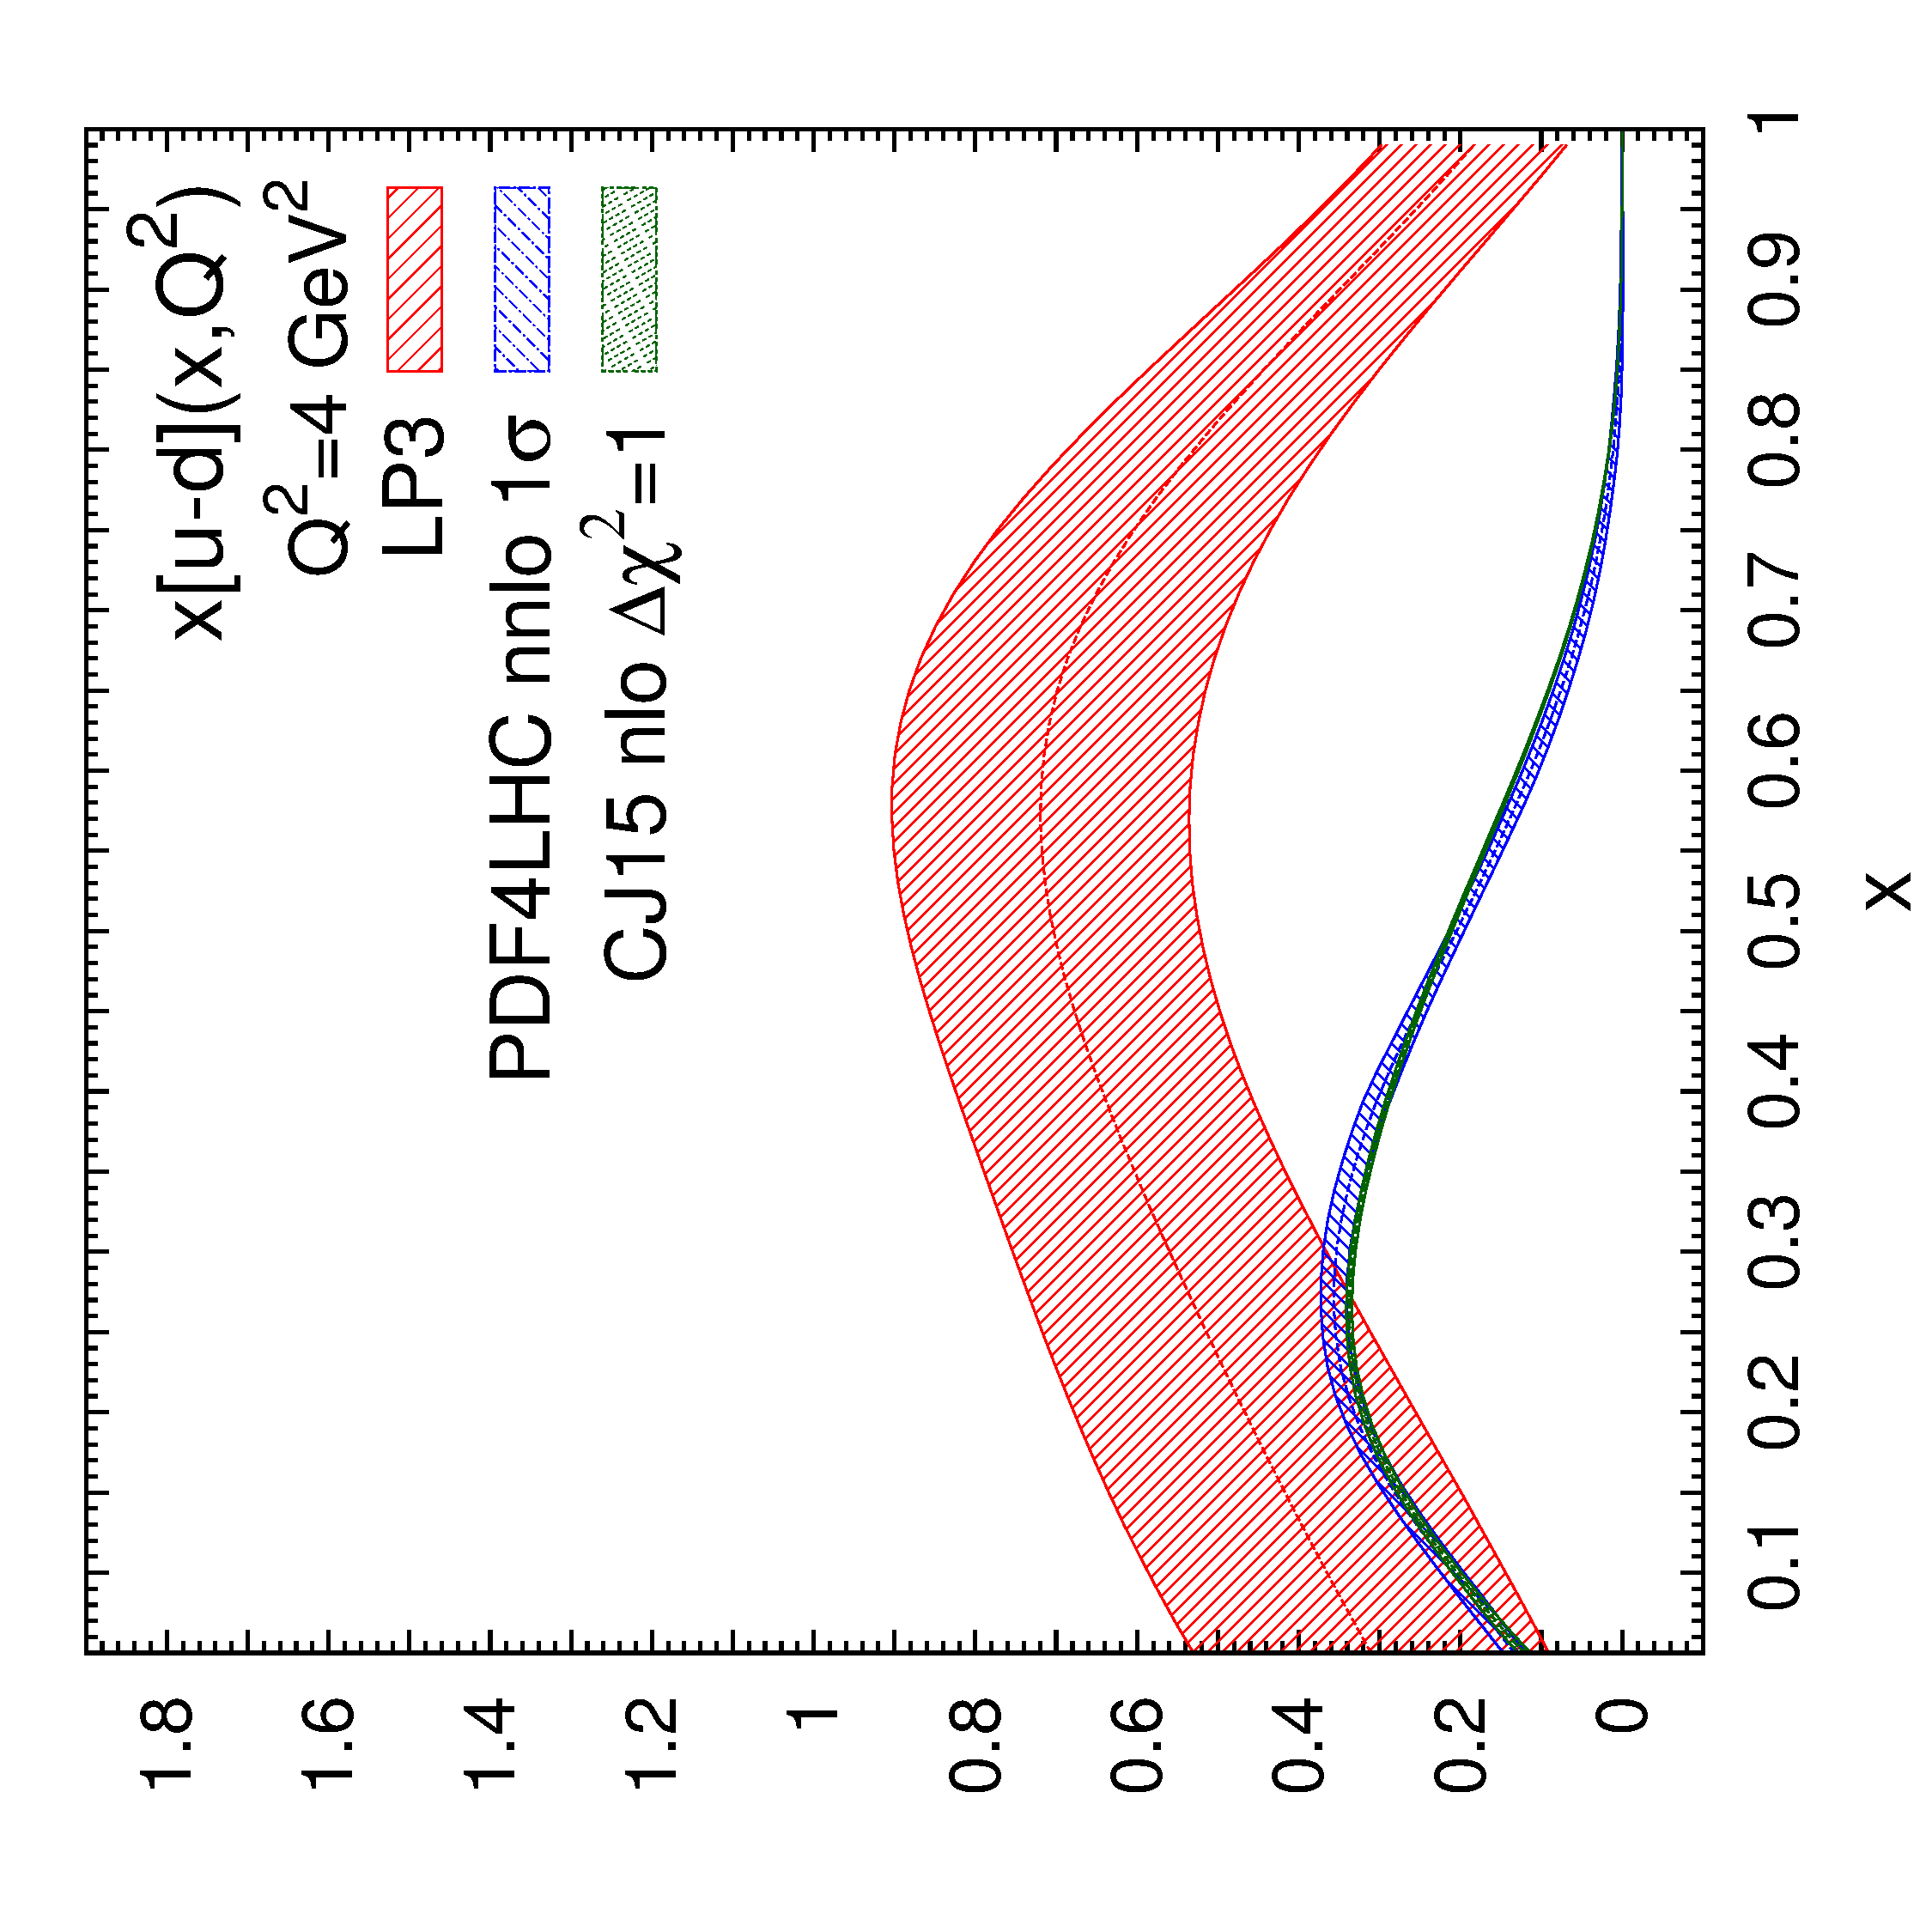
\includegraphics[scale=0.22,angle=270]{plots/unpxq}
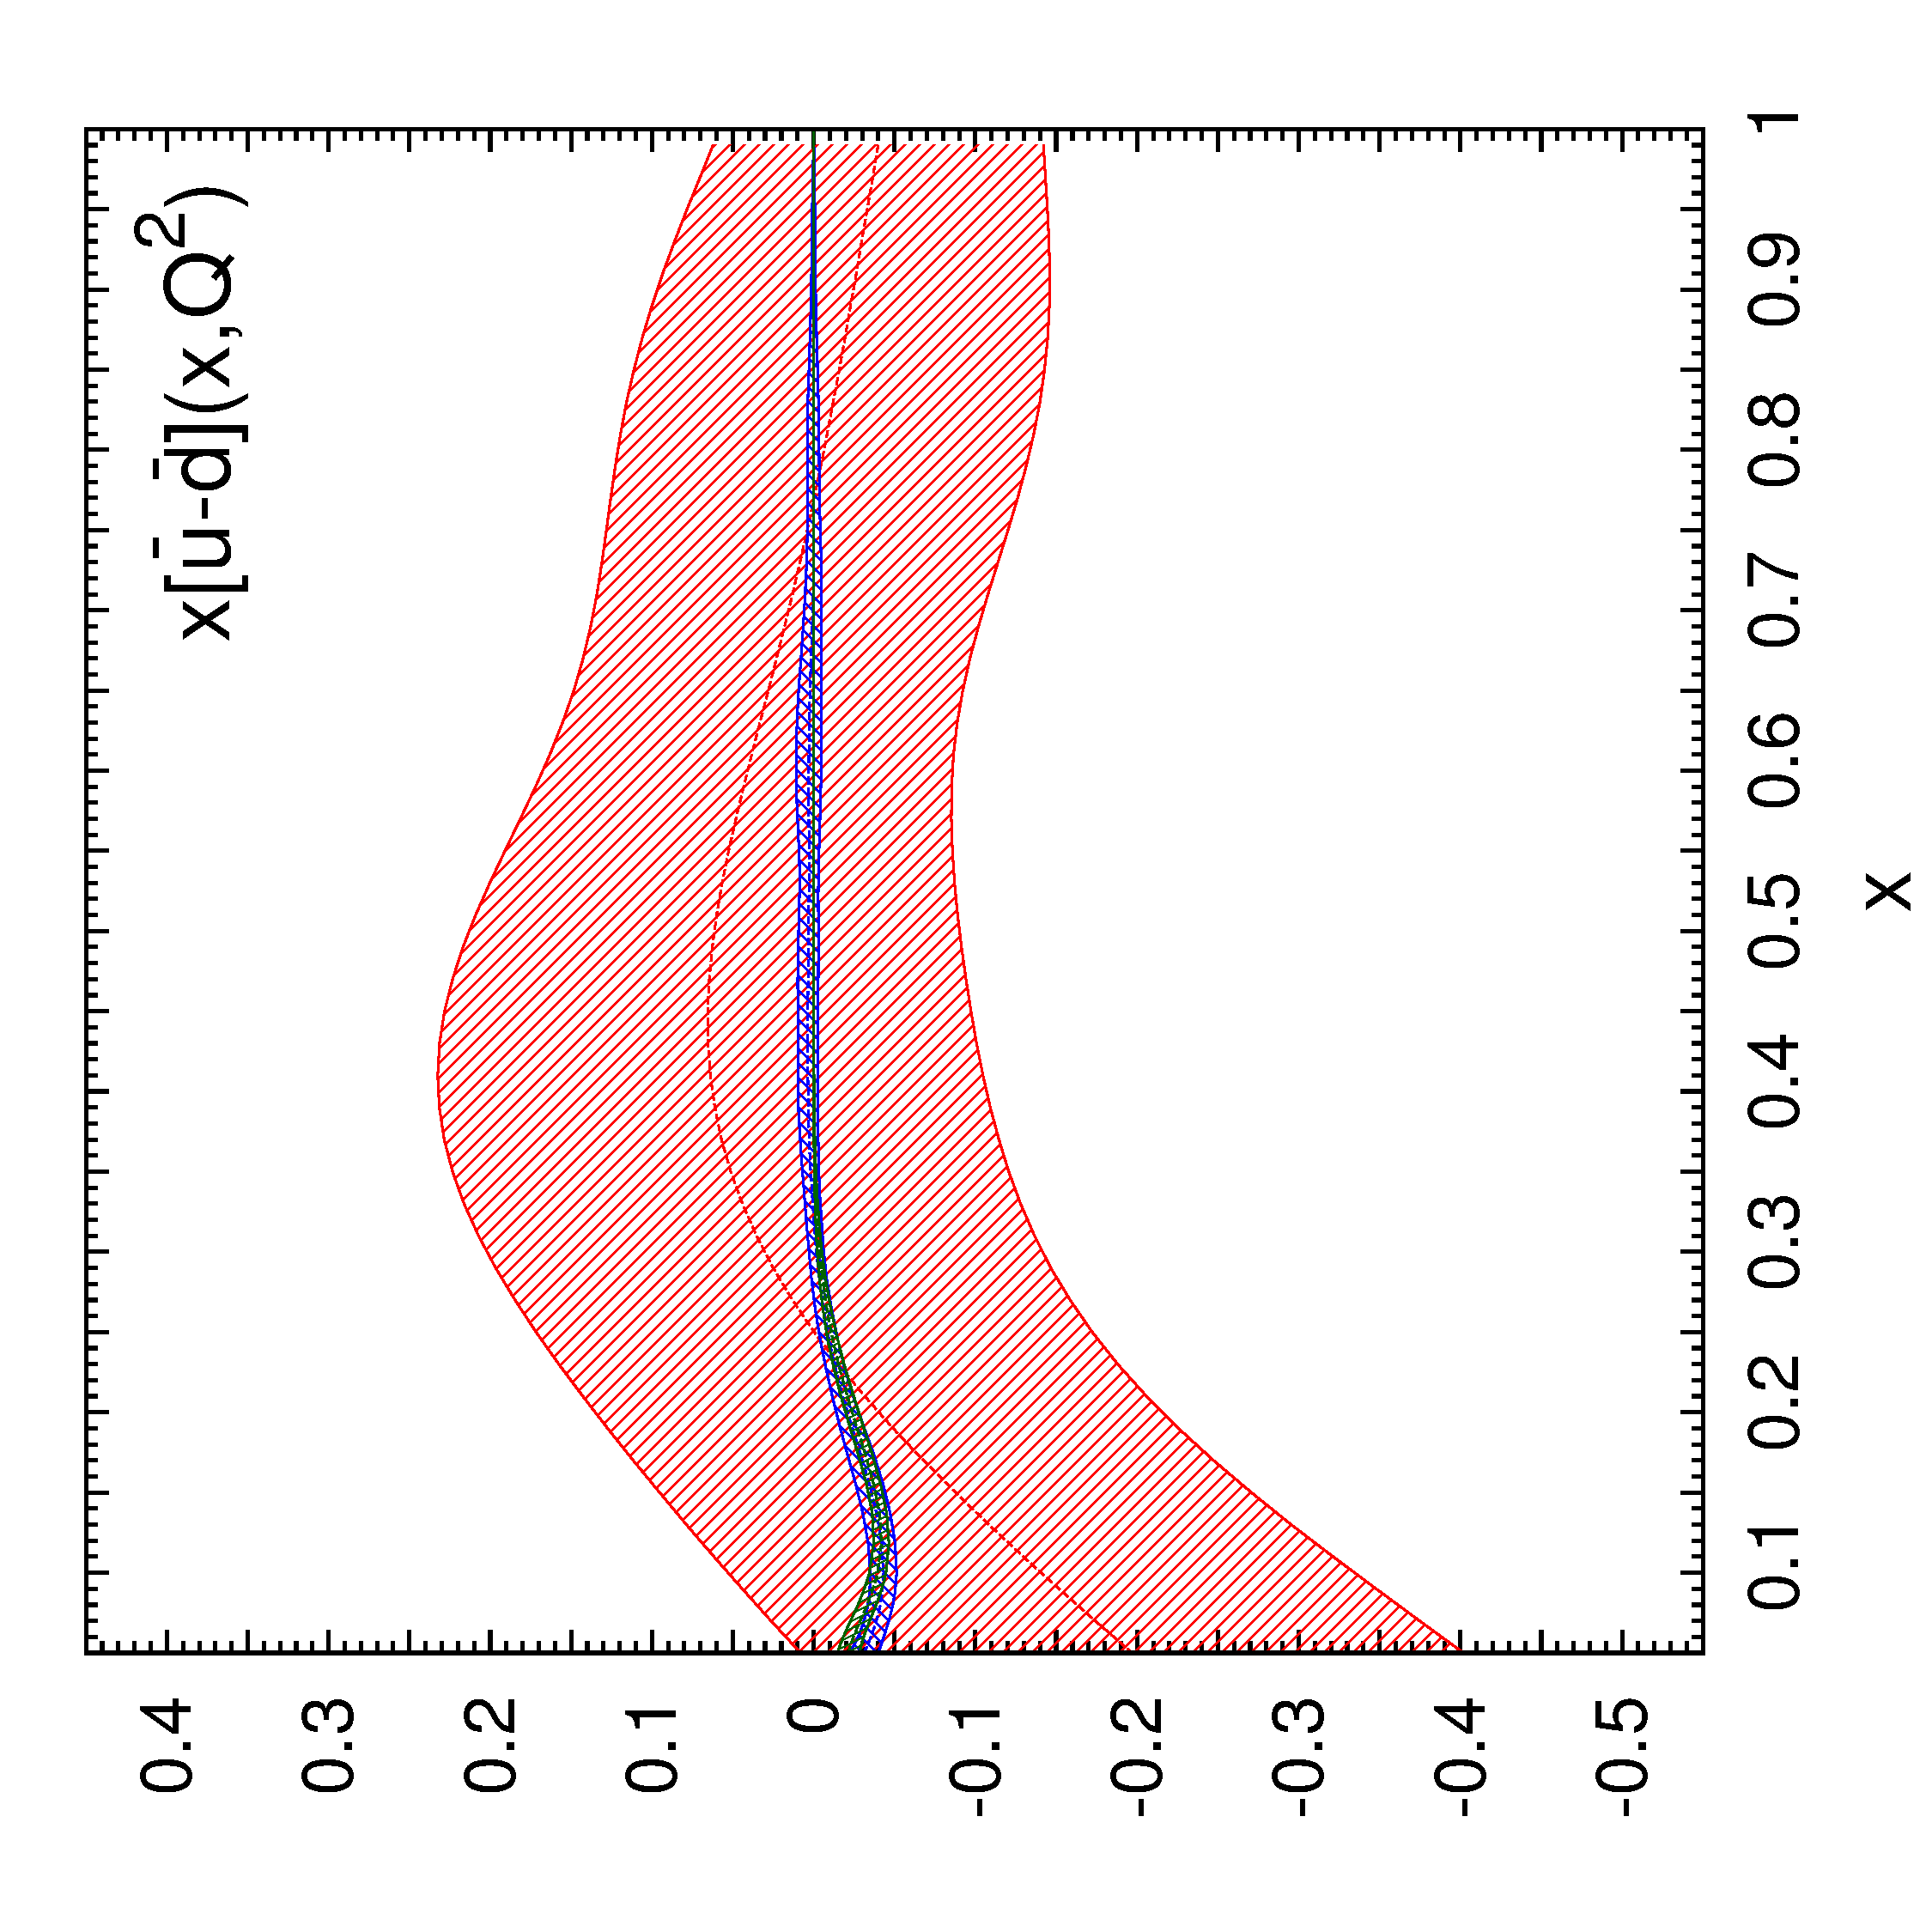
\includegraphics[scale=0.22,angle=270]{plots/unpxqbar}\\
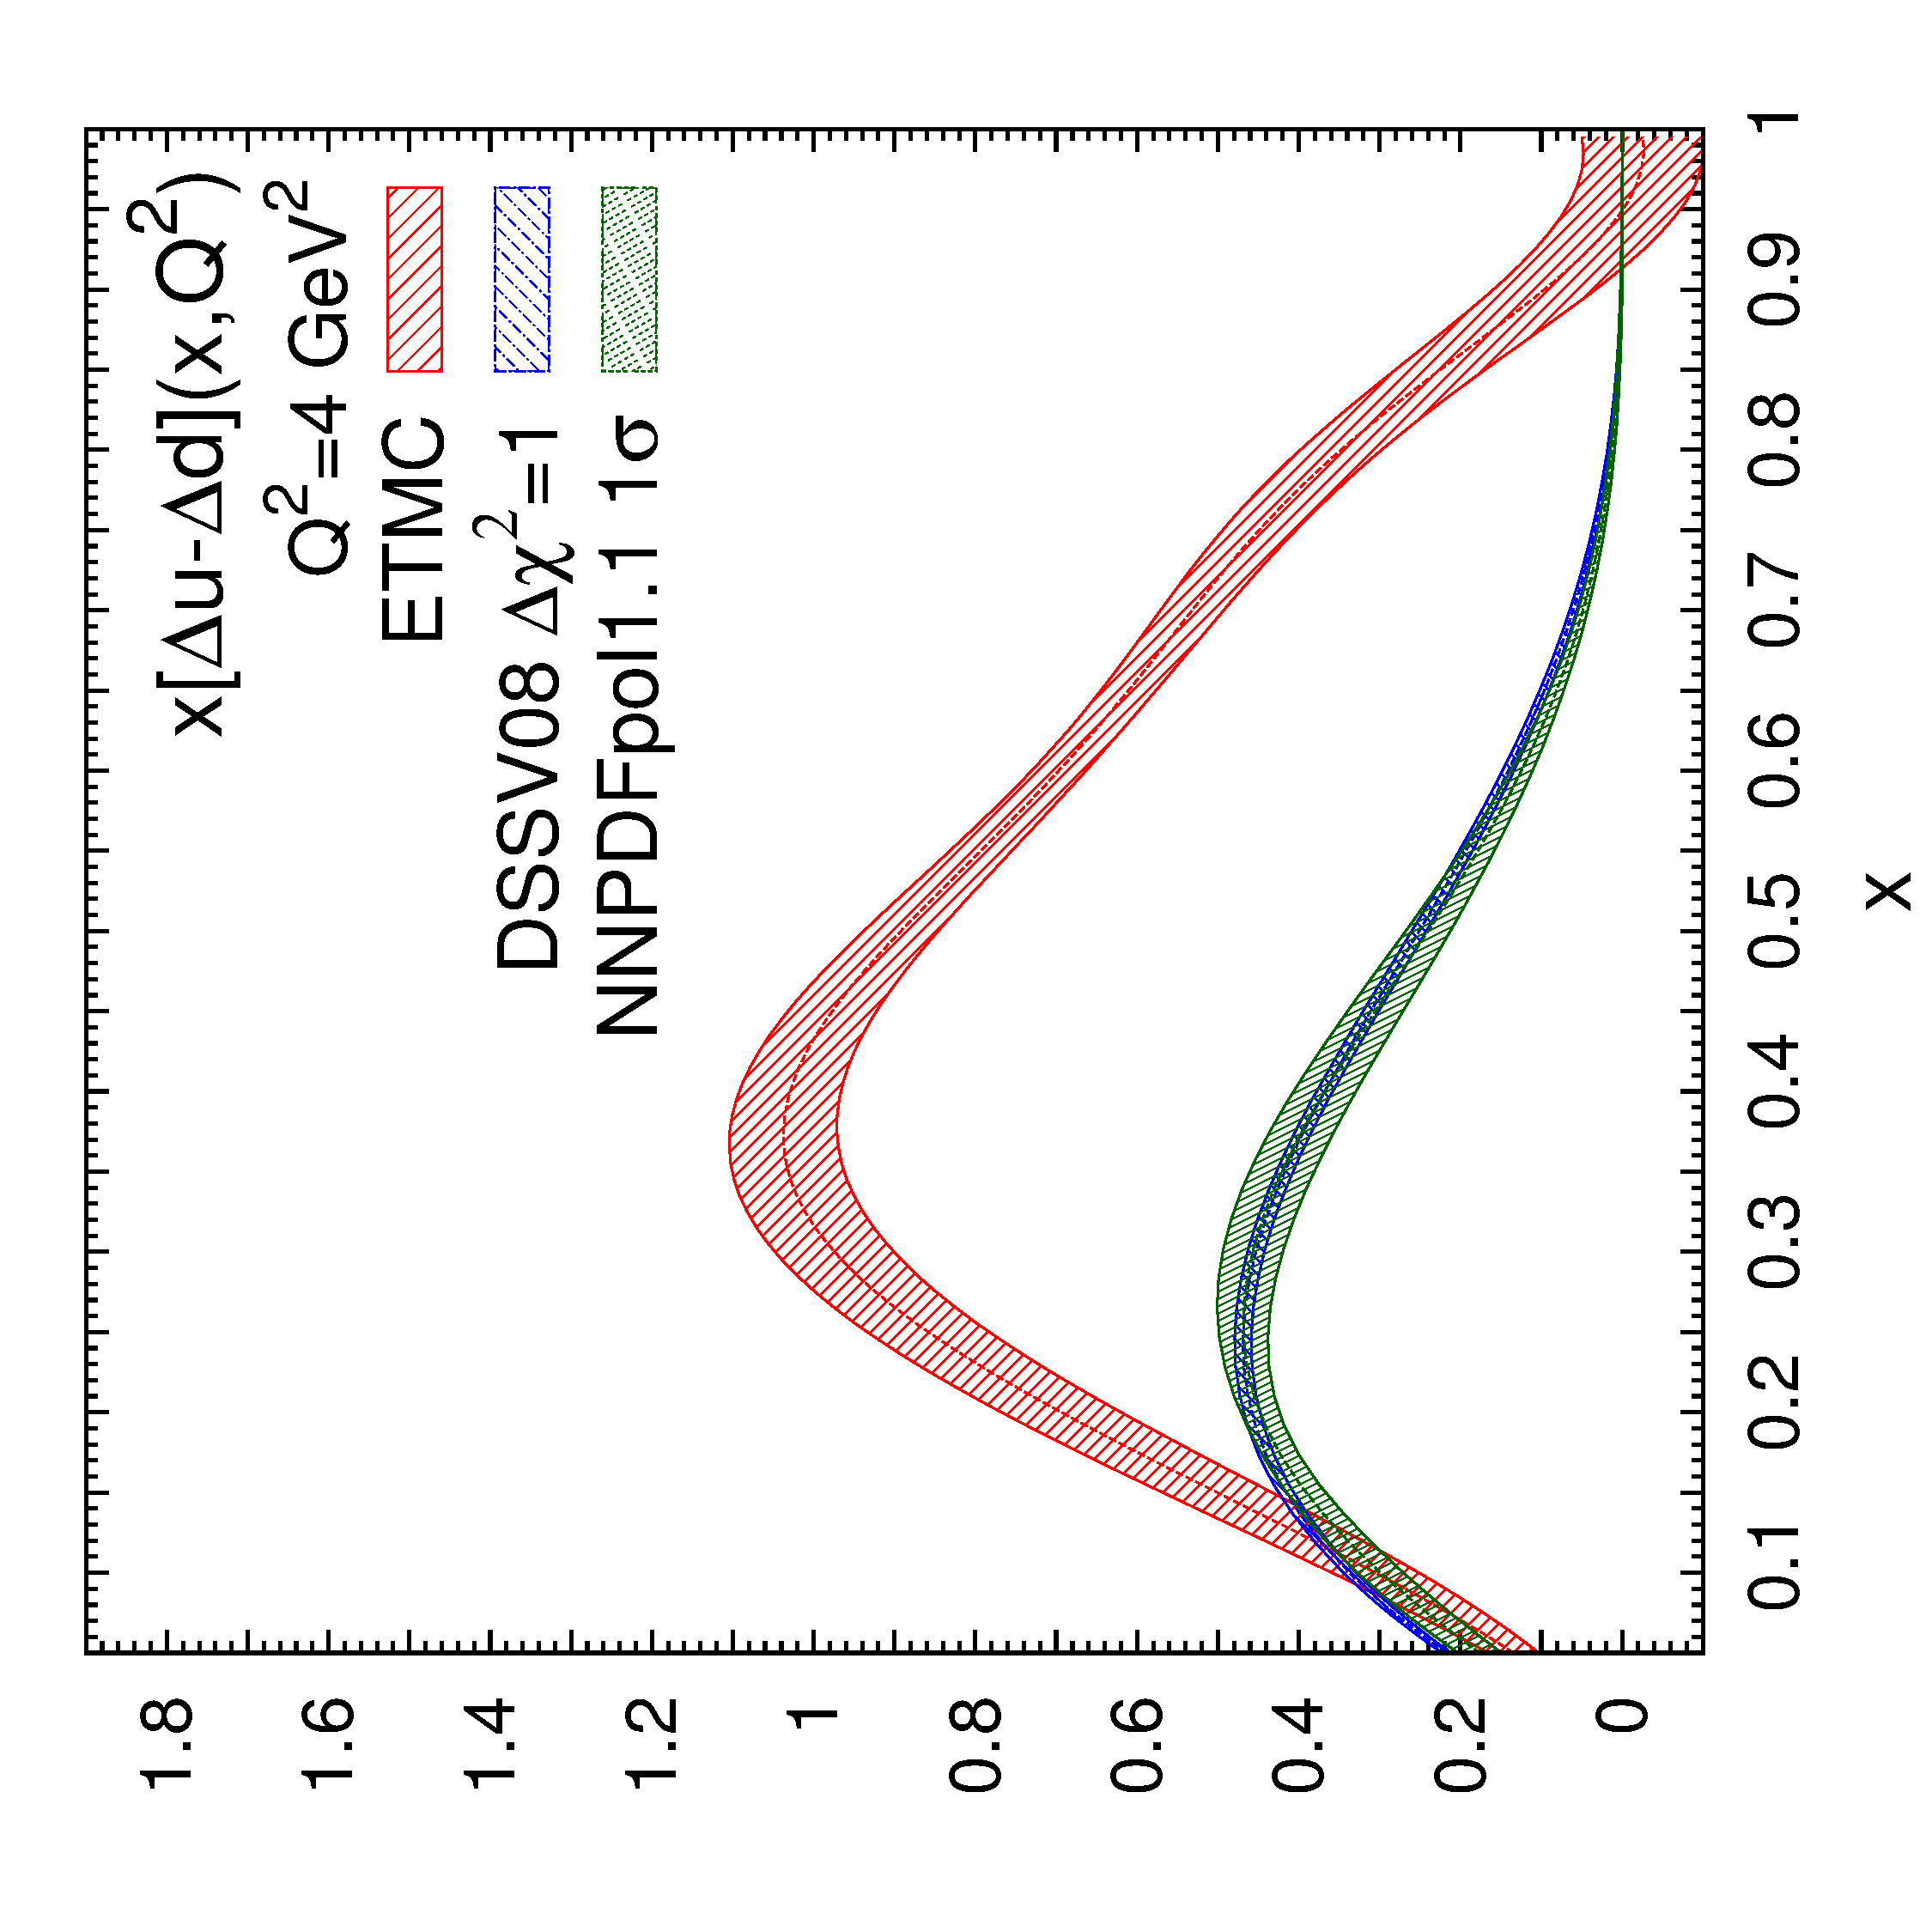
\includegraphics[scale=0.22,angle=270]{plots/polxq}
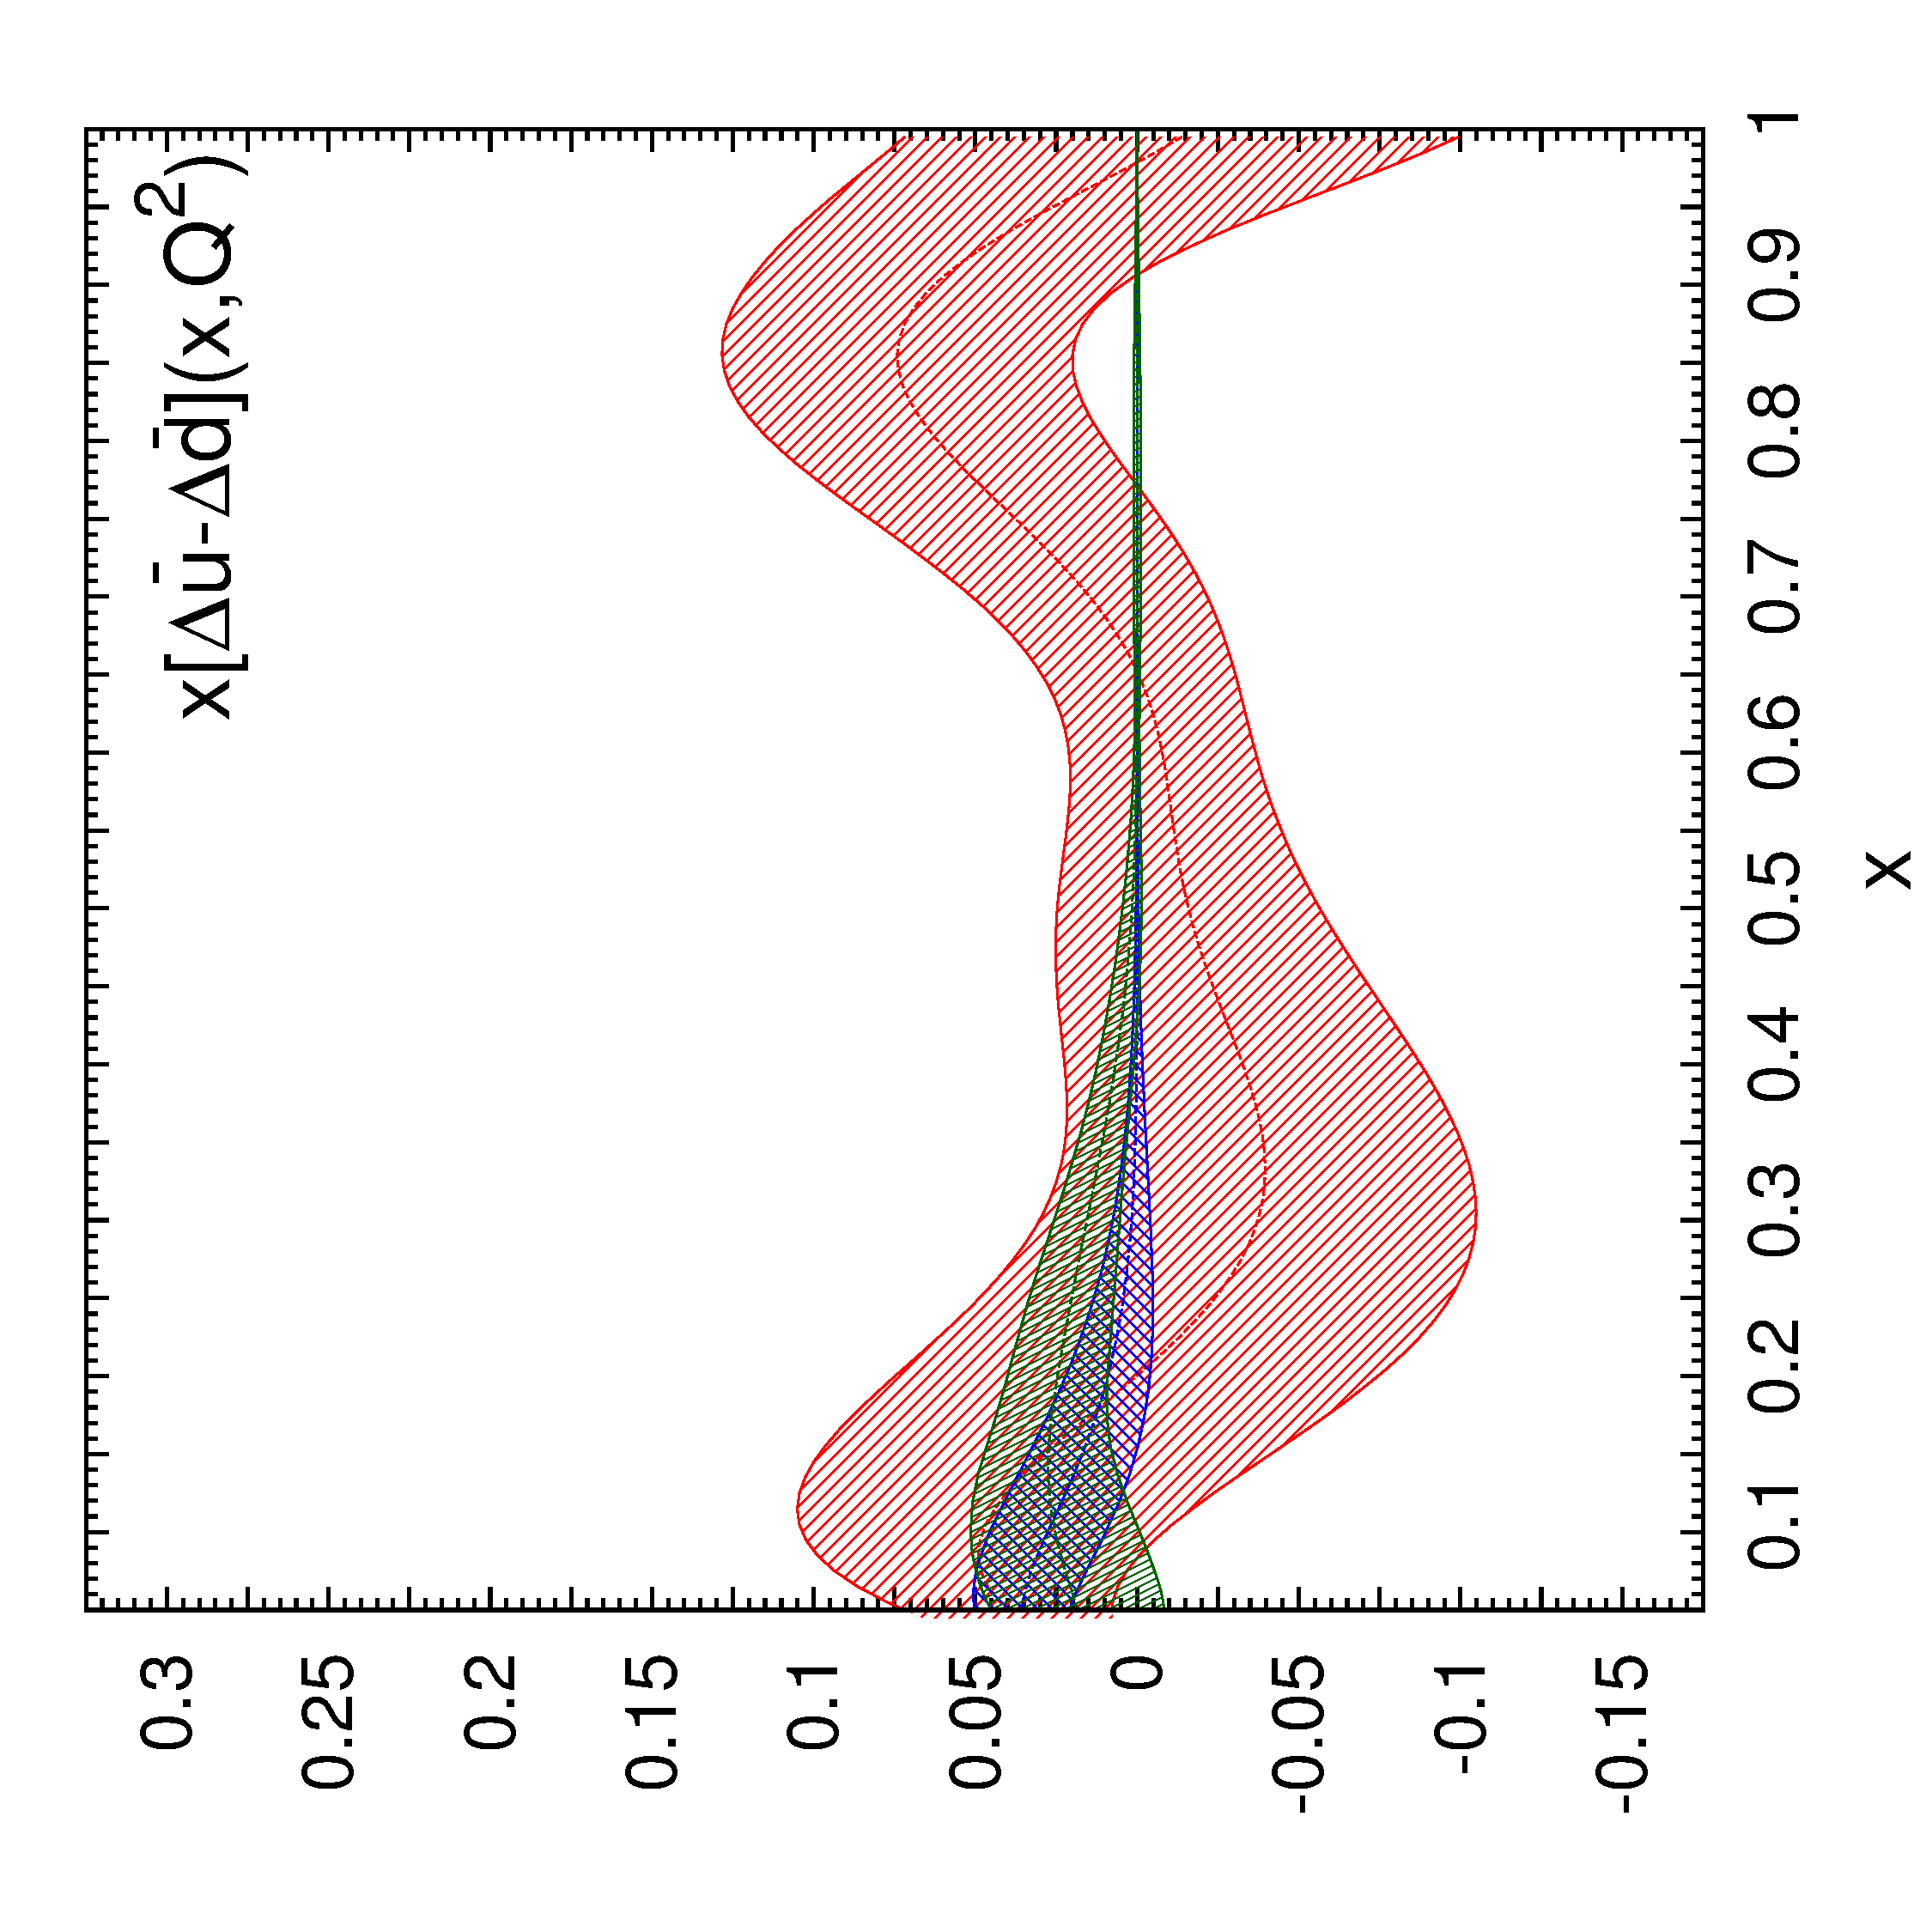
\includegraphics[scale=0.22,angle=270]{plots/polxqbar}\\
\caption{\small LP3's renormalized unpolarized isovector quark (top left) and 
  antiquark (top right) PDF combinations at physical pion mass with the renormalization scale 
  $\mu=2$~GeV~\cite{Lin:2017ani}. 
  %
  ETMC's renormalized polarized isovector quark (bottom left) and antiquark
  (bottom right) PDF combinations at pion mass of 
  375 MeV~\cite{Alexandrou:2017huk}.
  %
  Note that only statistical errors are shown here; the systematics are yet to be addressed. The small-x region (x< 0.2) can suffer larger systematics than the rest of the distribution due to the limited nucleon boost momentum.
  } 
\label{fig:qPDF-demo}
\end{figure}
%-------------------------------------------------------------------------------

\paragraph*{Pseudo-PDFs.} 
The general dependence of the  matrix element $h(z,p_z)$ of Eq.~\eqref{eq:qPDF} 
on the hadron momentum $p$ and the displacement of the quark and antiquark 
fields $z$ can be expressed as a function of the Lorentz invariants 
$\nu=z\cdot p$ (Ioffe time~\cite{Ioffe:1969kf,Braun:1994jq}) 
and $z^2$, where $z$ and $p$ are general 4-vectors.  
%
We can thus introduce
\begin{equation}
\overline{h}(\nu,z^2) \equiv h(z,p_z)\,.
\end{equation}

The pseudo-PDF is then defined by the Fourier transform
%
\begin{equation}
{\mathcal P}(x,z^2)=\int \frac{d\nu}{2\pi} e^{-ix\nu} \overline{h}(\nu,z^2),
\end{equation}
which has support only in the physical range 
$x=[-1,1]$ \cite{Radyushkin:2016hsy,Radyushkin:2017cyf}. 
%
As discussed in~\cite{Radyushkin:2016hsy,Radyushkin:2017cyf}, the pseudo-PDF 
is directly related to both the PDFs and the 
Transverse-Momentum-Dependent PDFs (TMDs).
%
In~\cite{Radyushkin:2017cyf}, using the temporal gamma matrix in the matrix 
element, a possible factorization of the TMD and PDF was conjectured which 
implies that the ratio
%
\begin{equation}
{\mathcal M}(\nu,z^2) =\frac{\overline h(\nu,z^2)}{\overline h(0,z^2)}
\label{eq:RatioPseudo}
\end{equation}
is directly related to the PDFs as 
\begin{equation}
{\mathcal M}(\nu,z^2) =Q(\nu,z^2) + {\cal O}(z^2).
\label{eq:IoffePDF}
\end{equation}
%
Here $Q(\nu,z^2)$ is the Ioffe time PDF~\cite{Ioffe:1969kf,Braun:1994jq}, 
which is just the Fourier transform of the PDFs,
\begin{equation}
{q}(x,1/z^2)=\int \frac{d\nu}{2\pi} e^{-ix\nu} Q(\nu,z^2).
\end{equation}
%
The ratio in Eq.~\eqref{eq:RatioPseudo} has a well-defined continuum 
limit and requires no renormalization. 
%
The polynomial corrections in Eq.~\eqref{eq:IoffePDF} are due to violations of 
the factorization conjecture, while the PDF ${q}(x,1/z^2)$ is the PDF in a 
particular scheme defined at scale $1/z^2$. Matching to $\overline{\rm MS}$ 
can be performed in perturbation theory following standard methodology. 
%
One loop results can be found in~\cite{Ji:2017rah,Radyushkin:2017lvu}.
%
A preliminary study was presented in~\cite{Orginos:2017kos,Karpie:2017bzm}, 
where it was shown that indeed the conjectured factorization is observed and 
the residual corrections are small. 
%
Further  evidence of the expected 
perturbative evolution of the Ioffe time PDFs was also observed. 
%
However, more detailed studies of this methodology are required.  


\subsection{Global PDF fits}
\label{Sec:IntroGlobalFits}

Global PDF fits realize a QCD analysis of hard-scattering measurements,
often using a variety of hadronic observables.
%
Parton distributions are parametrized at an initial energy scale, 
evolved up to the scale of the data via DGLAP 
equations~\eqref{eq:dglapunp}--\eqref{eq:dglappol}, and used to build up the 
theoretical predictions for the relevant observables.
%
In the corresponding factorization formul\ae, the factorization scale, $\mu$,
is usually set equal to the characteristic scale of the process, $Q$.
%
The best-fit parameters of PDFs are then determined by minimization of a 
proper figure of merit, such as the log-likelihood $\chi^2$.
%
In this section, we present the general global PDF fitting framework.
%
We discuss how PDFs are determined from hard-scattering observables,
paying attention to the assessment of PDF uncertainties.
%
We highlight the theory and the data used to fit both unpolarized and 
polarized PDFs and present a brief review of their state-of-the-art 
determination.

\subsubsection{General framework}
\label{sec:genframework}

\paragraph*{Fitting PDFs from hard-scattering data.} 
Parton distributions appear in the factorization formul{\ae} of a class of 
sufficiently inclusive processes, among which are deep-inelastic scattering 
(DIS) and proton-(anti)proton collisions.
%
The factorization formul{\ae} for the unpolarized and polarized structure 
functions $F_1$ and $g_1$ were introduced in Eqs.~\eqref{eq:Fi}--\eqref{pdf}.
%
For the hadroproduction of a generic final-state $X$ in unpolarized 
proton-proton ($pp$) collisions, the corresponding factorized expression reads
\begin{align}
\sigma_{pp\to X}(s,\mu^2_F,\mu^2_R)=&\sum_{a,b}\int {\rm d}x_1 {\rm d}x_2\, 
f_a(x_1,\mu_F^2)f_b(x_2,\mu_F^2)\,
\hat{\sigma}_{ab\to X}(x_1,x_2,s;\mu^2_{F},\mu^2_R)\;,
\label{eq:LHCxsecunp}
\end{align}
where the unpolarized hard cross-section 
$\hat{\sigma}_{ab\to X}$ can be calculated 
perturbatively as an expansion in the QCD and electroweak (EW) 
running couplings.
%
The specific values of the momentum fractions
$x_i$ can be related to the kinematics of the final state.
%
For example, for the production of a heavy final state, 
it can be shown that, at LO,
\be
x_{1,2}=\frac{M_X}{\sqrt{s}}e^{\pm y_X} \, ,
\ee
where $M_X$ and $y_X$ are the invariant mass and rapidity of the produced 
system and $\sqrt{s}$ is the center-of-mass energy.
%
The factorization and renormalization scales, $\mu_F$ and $\mu_R$, are 
usually taken equal to the hard scale of the process, $\mu_F=\mu_R=\mu=Q$.
%
Factorization formul{\ae} analogous to Eq.~\eqref{eq:LHCxsecunp} can be
written in the polarized case for $pp$ collisions where only one or
both proton beams are longitudinally polarized, see {\it e.g.}
Refs.~\cite{Stratmann:2001pb,Nadolsky:2003fz}.

When one performs a global fit, the DGLAP evolution equations of the PDFs, 
Eqs.~\eqref{eq:dglapunp}--\eqref{eq:dglappol}, derive the PDFs at any scale
relevant to comparisons with the data from PDF parametrizations at an
arbitrary input scale, typically $Q_0\sim 1$~GeV.
%
The contribution of heavy quark flavors to any process are 
power-suppressed at scales which are below the threshold for their 
production~\cite{Collins:1978wz}. 
%
Therefore, whereas in principle the QCD Lagrangian contains six quark flavors, 
in practice only a smaller number of active flavors $N_f$ are included in 
loops, and thus in particular in the solution of evolution equations. 
%
When expressing predictions for processes at various disparate scales in terms 
of a single set of PDFs it is thus necessary to use a so-called variable-flavor 
number (VFN) scheme, whereby different numbers of active flavors are adopted 
at different scales (with up to $N_f=5$ active flavors in most of PDF sets). 
%
Use of a fixed-flavor number (FFN)
scheme only allows comparison with the data in a restricted range of scales.

The input PDF parameterization is usually chosen as
\begin{equation}
\label{eq:pdffunc}
f(x,Q_0,\{a_i\})= x^{a_1}(1-x)^{a_2}\:C(x,\{a_j\})\, ,
\end{equation}
where the parameters $\{a_i\}$ determine the PDF shape
and are different for each PDF flavor combination probed by the data.
%
The $(1-x)^{a_2}$ term, with $a_{2}>0$, ensures that the PDFs vanish in the 
elastic limit $x\to 1$. 
%
Specific values of the exponent $a_2$ are predicted by counting 
rules~\cite{Brodsky:1973kr}, although they are not always clearly
supported by phenomenological fits~\cite{Ball:2016spl,Nocera:2014uea}, 
and are not always used.
%
The $x^{a_1}$ term governs the low-$x$ PDF behavior. 
%
It is expected from considerations based on Regge theory, 
which also provides the values of the exponents $a_1$.
%
However, as for $a_2$, the value of $a_1$ is left free in the global fits.
%
The interpolating function $C(x)$ in Eq.~\eqref{eq:pdffunc}
affects the behavior of the PDFs away from the $x\to 0$ and $x\to 1$
extrapolation regions.
%
This is assumed to be a smoothly varying function of $x$, for which a variety 
of parametrizations can be made.

The simplest ansatz, which has been very widely used, is to take a basic 
polynomial form in $x$ (or $\sqrt{x}$), such as
\begin{equation}\label{eq:lpower}
C(x)=1+a_2\sqrt{x}+a_3 x+...\;.
\end{equation}
Functional forms of this type are, for example, taken in CJ, HERAPDF and 
earlier MMHT and CT sets (see below for the references to each set). 
%
More recently, the CT and MMHT collaborations expand 
in terms of a basis of  Bernstein and Chebyshev polynomials, respectively.
%
While formally equivalent to the simple polynomial expansion
Eq.~\eqref{eq:lpower}, these are much more convenient for fitting as the 
number of free parameters $n_{\rm par}$ is large.
%
In the latest CT and MMHT sets, there are between 20 and 40 free parameters in 
total, though some of these are kept fixed when evaluating the
Hessian PDF uncertainties to reduce redundancy between the parameters.
%
Furthermore, the use of orthogonal polynomials, like Chebyshev 
polynomials, allows one to decouple the parameters in $C(x)$ and to uniformly
sample its possible functional shapes.

An alternative approach to the PDF parametrization Eq.~\eqref{eq:lpower}
is adopted by the NNPDF collaboration. 
%
Here, the interpolating function $C(x)$ is modeled with 
a multi-layer feed-forward neural network (NN).
%
In practice, this allows for a greatly increased number of free parameters, 
typically an order of magnitude higher than in the sets of other groups.
%
The form of Eq.~\eqref{eq:pdffunc} is still assumed, but
now $C(x)={\rm NN}(x)$, where ${\rm NN}(x)$ is a neural network.
%
The $x^{a_1}(1-x)^{a_2}$ term that multiplies ${\rm NN}(x)$ represents
a preprocessing factor that speeds up the minimization procedure
and that is determined via an iterative procedure.
%
Because of its parametric redundancy, the neural network parametrization
can be overtrained and learn the statistical noise of the data.
%
In order to avoid such a drawback, the data are split into validation and 
training sets, then the best-fit is determined by
cross-validation~\cite{Forte:2002fg,DelDebbio:2004xtd}.
%
A similar technique is used also in the JAM 
fits~\cite{Sato:2016tuz,Ethier:2017zbq}.

In most of PDF sets currently in use, the PDFs for charm and heavier quarks
are not parametrized as in Eq.~\eqref{eq:pdffunc}, but rather they are
generated by perturbative emission of gluons and light quarks.
%
In the vicinity of the threshold for heavy-quark production, the quark mass
cannot be neglected.
%
It is thus necessary to explicitly include terms suppressed by
powers of the heavy-quark mass in the coefficient functions, while 
subtracting the logarithmically enhanced, unsuppressed terms that are 
already generated by solving the evolution equations in order 
to avoid double counting.
%
Various schemes exist so far to do so, see {\it e.g.}
Refs.~\cite{Forte:2013wc,Gao:2017yyd} for an extensive summary.
%
The possibility of parametrizing and fitting the charm PDF
on the same footing as light quark PDFs has been also explored, see 
{\it e.g.}~\cite{Brodsky:2015fna,Ball:2016neh,Hou:2017khm}
and references therein.

Once the PDF parametrization is chosen, and the theoretical details 
of the analysis are defined (such as the perturbative order, the
treatment of heavy quarks, etc.), the best-fit PDF parameters
and their uncertainty should be determined via a fitting methodology
that minimizes a suitable statistical estimator, typically the $\chi^2$.
%
There exist different alternative definitions of the $\chi^2$
to be used in the global 
fits~\cite{Ball:2012wy,Gao:2013xoa,Alekhin:2017kpj,Abramowicz:2015mha}. 
%
For instance one frequently used definition is
\begin{equation}
\chi^2 
= 
\sum_{i,j}^{N_{\rm dat}} (T_i(\{a_k\}) - D_i) 
({\rm cov^{-1}})_{ij} (T_j(\{a_k\}) - D_j)\,,
\label{eq:chi2}
\end{equation}
where $N_{\rm dat}$ is the number of data points of a given experiment,
$T_i$ and $D_i$ are the corresponding theoretical predictions
and experimental data, and $({\rm cov^{-1}})_{ij}$ is the inverse of the 
experimental covariance matrix.
%
The theoretical predictions $T_i(\{a_k\})$ depend on the input set of 
parameters $\{a_k\}$ via the PDF parametrization, see Eq.~\eqref{eq:pdffunc}.
%
Therefore, Eq.~\eqref{eq:chi2} assesses the agreement between theory and data.

The covariance matrix $({\rm cov})_{ij}$ accounts for the various sources of 
experimental systematic uncertainties and also allows for several
different definitions.
%
One example is the so-called $t_{0}$ prescription~\cite{Ball:2009qv}, 
where a fixed theory prediction $T_{i}^{(0)}$ is used to define the  
contribution to the $\chi^2$ from the multiplicative systematic uncertainties, 
namely
\be
\label{eq:covmat_t00}
({\rm cov})_{ij}=
\delta_{ij} \sigma_{\rm stat}^2 + 
\sum_{\alpha=1}^{N_c}\sigma^{(c)}_{i,\alpha}\sigma^{(c)}_{j,\alpha}D_{i} D_{j}
+ \sum_{\beta=1}^{N_{\cal L}} \sigma_{i,\beta}^{({\cal L})}\sigma_{j,\beta}^{({\cal L})}
T^{(0)}_{i} T^{(0)}_{j}\, .
\ee
Here $\sigma_{\rm stat}$ is the uncorrelated uncertainty,
and $\sigma^{(c)}_{i,\alpha}$ ($\sigma^{(\cal L)}_{i,\beta}$) are the various sources 
of additive (multiplicative) systematic uncertainties.
%
The $t_0$ prescription is needed to avoid the D'Agostini 
bias~\cite{DAgostini:2003syq,DAgostini:1993arp}, a downwards
bias of the statistical estimators for the central value and the uncertainty
of the theoretical predictions due to the rescaling induced by  multiplicative 
uncertainties.
%
See~\cite{Ball:2009qv,Ball:2012wy} and references therein for details and the 
alternative {\it penalty-trick} prescription, and~\cite{Gao:2013xoa}
for the alternative {\it extended}-$t$ prescription.

\paragraph{PDF uncertainties.}
Determining the best-fit values of the PDF parameters is not enough: one also 
needs to estimate the associated PDF uncertainties, possibly separated into 
the various sources of experimental, methodological and theoretical 
uncertainties.
%
In this respect, there are two main methods to determine PDF uncertainties, the 
{\it Hessian} and the {\it Monte Carlo} (MC) methods.\footnote{The Lagrange 
multiplier method~\cite{Stump:2001gu} is also frequently used for dedicated 
studies of PDF uncertainties.}

The Hessian method~\cite{Pumplin:2001ct} is based on the parabolic
expansion of the $\chi^2$ in the vicinity of its minimum 
\be
\label{eq:hessianexpansion}
\Delta\chi^2 \equiv \chi^2- \chi^2_{\rm min}
=\sum_{i,j=1}^{n_{\rm par}}H_{ij}\lp a_i-a_i^0\rp
\lp a_j-a_j^0\rp \, ,
\ee
where the $n_{\rm par}$ PDF fit parameters are denoted by 
$\{a_1,\ldots,a_{n_{\rm par}}\}$, the best-fit values that minimize the
$\chi^2$ are indicated by $\{a_1^0,\ldots,a^0_{n_{\rm par}}\}$,
and the Hessian matrix is defined as
\be
H_{ij}\equiv \frac{1}{2} \frac{\partial^2\chi^2}{\partial a_i
\partial a_j}\Bigg|_{\{\vec{a}\}=
\{\vec{a}^0\}}\, .
\ee
By diagonalizing this Hessian matrix, it becomes possible
to represent PDF uncertainties in terms of orthogonal eigenvectors
within a fixed tolerance $T=\sqrt{\Delta\chi^2}$.
%
These eigenvectors can then be used to estimate the PDF uncertainty for 
arbitrary cross-sections, using the master formula of Hessian PDF sets for 
the uncertainty of the cross-section $\mathcal{F}$, such 
as~\cite{Pumplin:2002vw}
\be
\label{eq:hessianmaster2}
\sigma_{\mathcal{F}}=\frac{1}{2}\lp \sum_{i,j}^{n_{\rm par}}
\lc \mathcal{F}(S_i^+)-\mathcal{F}(S_i^-) \rc^2 \rp^{1/2} \, ,
\ee
where $S_i^{\pm}$ correspond to the $i$-th eigenvector
associated with positive and negative variations with respect
to the best fit value.

The Monte Carlo method~\cite{Giele:1998gw,Giele:2001mr,Forte:2002fg,
DelDebbio:2004xtd} is based 
on constructing a representation of the probability distribution of the 
experimental data in terms of a large number $N_{\rm rep}$ of {replicas},  
which encode all the information on central values, variances and 
correlations provided by the experiments.
%
Specifically, given an experimental measurement of a hard-scattering
observable $F_{I}^{\rm (exp)}$, with total uncorrelated uncertainty 
$\sigma_{I}^{\rm (stat)}$, $N_{\rm sys}$ fully correlated systematic uncertainties 
$\sigma^{\rm (corr)}_{I,c}$ and $N_a$ ($N_r$) absolute (relative) normalization 
uncertainties $\sigma^{\rm (norm)}_{I,n}$, the Monte Carlo replicas are 
constructed using the expression
\be
\label{eq:replicas}
F_{I}^{(\art)(k)}
=
S_{I,N}^{(k)} F_{I}^{\rm (\mrexp)}\lp 1
+
\sum_{c=1}^{N_{\rm sys}}r_{I,c}^{(k)}\sigma^{\rm (corr)}_{I,c}
+
r_{I}^{(k)}\sigma_{I}^{\rm (stat)}\rp
\ , \quad k=1,\ldots,N_{\rep} \ ,
\ee
where $S_{I,N}^{(k)}$ is a normalization prefactor.
%
The variables $r_{I,c}^{(k)},r_{I}^{(k)},r_{p,n}^{(k)}$ are
univariate Gaussian random numbers.
%
For each individual replica, the random fluctuations associated with a given 
fully-correlated systematic uncertainty will be the same
for all data points, $r^{(k)}_{I,c}=r^{(k)}_{I',c}$.

Parton distribution fits are then performed separately on each of the 
Monte Carlo replicas.
%
The resulting ensemble of PDFs samples the probability density in the space
of PDFs.
%
The expectation function of a generic observable $ \mathcal{F} [ \{  f \}]$,
depending on the fitted set of PDFs $\{f\}$,
is evaluated as an average over the replica sample,
\be
\label{masterave}
\la \mathcal{F} [ \{  f \}] \ra
= \frac{1}{N_{\rm rep}} \sum_{k=1}^{N_{\rm rep}}
\mathcal{F} [ \{  f^{(k)} \}] \, .
\ee
The corresponding uncertainty is determined as the variance of the
Monte Carlo sample,
\be
\sigma_{\mathcal{F}} =
\left( \frac{1}{N_{\rm rep}-1}
\sum_{k=1}^{N_{\rm rep}}   
\lp \mathcal{F} [ \{  f^{(k)} \}] 
-   \la \mathcal{F} [ \{  f \}] \ra\rp^2 
 \right)^{1/2}.
\label{mastersig}
\ee
Likewise, other properties of the underlying PDF probability distribution, 
such as skewness and kurtosis, could be readily computed.

Given a PDF set in the Hessian representation, it is possible to construct
the corresponding Monte Carlo representation~\cite{Watt:2012tq,Hou:2016sho}
and vice-versa~\cite{Gao:2013bia,Carrazza:2015aoa}.

So far, we discussed PDF uncertainties following from propagation of the
uncertainty of the experimental data that underlie the PDF determination.
%
Procedural uncertainties, associated with the methodology used to 
determine PDFs from data, can also be accounted for in the MC or Hessian
approaches, or reduced to a negligible size, as in the NNPDF approach.
%
There are however additional sources of uncertainty, mostly theoretical, 
that are not accounted for, either in the Hessian or in the MC methods.
%
These are extensively discussed 
in Refs.~\cite{Forte:2013wc,Butterworth:2015oua,Accardi:2016ndt,Gao:2017yyd} 
and briefly summarized as follows.

\begin{itemize}

\item The uncertainty due to finite uncertainties 
associated with the input values of the physical parameters used in the global 
fit, such as $\alpha_s(m_Z)$ and the charm mass $m_c(m_c)$, is 
evaluated by repeating the fits for different values of the physical 
parameters and then by suitably combining the results.

\item The missing higher order uncertainty (MHOU), due to the truncation
of the perturbative expansion, is usually inferred by comparing NLO to NNLO 
unpolarized PDFs and LO to NLO polarized PDFs.
%
While this is expected to be small for NNLO fits, currently its size is unknown.

\item The uncertainty due to different choices in the treatment of heavy quarks
was studied in Refs.~\cite{Binoth:2010nha,Thorne:2012az}, for unpolarized PDFs, 
by looking at their impact.
%
It was found that differences may not be entirely negligible at NLO in 
the vicinity of the quark threshold, though they rapidly decrease at 
NNLO~\cite{Binoth:2010nha}.

\item Uncertainties associated with missing higher-twist (power-suppressed) 
corrections (if they are not included in the factorized description of 
fit observables) are kept under control by removing data, below some low cutoff 
scale, that may be affected by them. 
%
Their impact can be studied by varying this 
cutoff~\cite{Martin:2003sk,Accardi:2009br}, or
by looking at the stability of the fit with and without inclusion of higher 
twist terms~\cite{Sato:2016tuz,Accardi:2016qay,Alekhin:2017kpj}.

\item Uncertainties associated with nuclear corrections, whenever they are
not included, affect some DIS data in which targets are deuterons or heavier 
nuclei, rather than just protons.
%
They have been studied by including such corrections according to various 
models~\cite{Martin:2009iq,Ball:2009mk,Sato:2016tuz,Accardi:2016qay}, 
or by attempting to fit the corrections 
directly~\cite{Martin:2009iq,Martin:2012da}.

\item Extrapolation uncertainties in the region not covered 
by experimental data are particularly delicate as far as full moments of PDFs
are concerned.
%
They are difficult to quantify, especially in the polarized case at small $x$
due to the lack of data.
%
The impact of extrapolation uncertainties in the unpolarized case at large $x$
has been studied in~\cite{Accardi:2011fa,Accardi:2016ndt}.

\end{itemize}
%
At present, the only way of dealing with such uncertainties is to make sure 
that they are small enough (in comparison to the data uncertainty)
in each PDF set.
%
Therefore, in the remainder of this paper, 
we will assume that they can be neglected.
%
We will point out to the reader how global-fit results can be affected 
by underestimation of these uncertainties in 
Secs.~\ref{subsubsec:GPDFfits}--\ref{subsec:BN}.

\subsubsection{Unpolarized PDFs}
\label{sec:unpPDFs}

\paragraph*{Theoretical features.}
While the general $x$ dependence of the PDFs is determined by
nonperturbative QCD dynamics, there are still a number
of theoretical constraints that any PDF set should satisfy. 
%
These should be imposed during the fit procedure.

First, since the proton has the quantum numbers of two up quarks and one 
down quark, the following quark number sum rules, given in terms of zeroth
moments, must be satisfied: 
\begin{eqnarray}
\int_{0}^{1}dx\ \left[u(x,\mu^2)-\bar{u}(x,\mu^2)\right] 
& =\left\langle 1\right\rangle _{u^{-}}= & 2 \, ,\nonumber \\
\int_{0}^{1}dx\ \left[d(x,\mu^2)-\bar{d}(x,\mu^2)\right] 
& =\left\langle 1\right\rangle _{d^{-}}= & 1 \, ,
\label{eq:valencesumrules}\\
\int_{0}^{1}dx\ \left[s(x,\mu^2)-\bar{s}(x,\mu^2)\right] 
& =\left\langle 1\right\rangle _{s^{-}}= & 0 \, .\nonumber
\end{eqnarray}
%
Similar constraints hold for heavy quarks: 
$\left\langle 1\right\rangle _{c^{-}}=\left\langle 1\right\rangle _{b^{-}}
=\left\langle 1\right\rangle _{t^{-}}=0$.
%
The valence sum rules, Eqs.~\eqref{eq:valencesumrules}, should be satisfied at 
any scale $\mu$. 
%
Indeed it can be shown that if they hold at the input parametrization scale 
$\mu=Q_0$, they are subsequently respected by DGLAP evolution.
%
Therefore, for these distributions we must have $a_1>-1$ in
Eq.~\eqref{eq:pdffunc}, otherwise Eqs.\eqref{eq:valencesumrules} 
would be ill-defined.

Second, PDFs should satisfy the conservation of energy-momentum derived from
the QCD Lagrangian.
%
In other words, the proton's total momentum should be equal 
to the sum of the momentum carried by all its constituents
(the so-called momentum sum rule):
\begin{equation}
\label{eq:mom}
1 
= 
\left\langle x\right\rangle _{g}
+
\left\langle x\right\rangle _{u^{+}}
+
\left\langle x\right\rangle _{d^{+}}
+
\left\langle x\right\rangle _{s^{+}}
+
\left\langle x\right\rangle _{c^{+}}
+
\left\langle x\right\rangle _{b^{+}}
+
\left\langle x\right\rangle _{t^{+}}+\ldots\,,
\end{equation}
%
where the ellipsis represents any other partonic components (such
as a photon). 
%
The first moments, $\left\langle x\right\rangle _{f}$, are defined in analogy 
to Eqs.~\eqref{eq:umoment1}--\eqref{eq:uplusmoment1}. 
%
In order to avoid a divergent contribution, we must have $a_1>-2$ in 
Eq.~\eqref{eq:pdffunc} for the non-valence distributions.
%
Typically it turns out that $-2<a_1<-1$ for such distributions, hence 
the number of soft partons grows very quickly at small $x$, although the 
momentum fraction carried by them is well-defined and finite.
%
As in the case of the valence sum rules, the momentum
sum rule is preserved by the DGLAP evolution equations.

Theoretical calculations of DIS and hadronic cross-sections at the highest 
perturbative order available should be used.
%
Currently, this implies using NNLO for the QCD corrections and NLO
for the EW and photon-induced effects~\cite{Manohar:2016nzj,Manohar:2017eqh}.
%
Thanks to recent progress in higher-order calculations, these results
are available for most of the processes entering the global
PDF fits~\cite{Currie:2016bfm,Campbell:2016lzl,Czakon:2016dgf,
Boughezal:2017nla,Li:2012wna}, including differential distributions with 
colored particles in the final state.

These calculations should be provided in
a format such that the evaluation of the hadronic
cross-sections, Eq.~\eqref{eq:LHCxsecunp}, is not too burdensome
from a computational point of view.
%
To bypass the limitations of the lengthy (N)NLO
computations, a number of fast interfaces have
been developed that allow for the efficient calculation
of NLO (and NNLO) fully differential hadronic cross-sections,
among which {\tt APPLgrid}~\cite{Carli:2010rw},
{\tt FastNLO}~\cite{Wobisch:2011ij} and {\tt aMCfast}~\cite{Bertone:2014zva}.

\paragraph*{Experimental data.}
A broad set of input hard-scattering cross-sections from DIS and
proton-(anti)proton collisions, providing information on the PDFs over a wide 
range of $x$ and for different flavor combinations, is used in modern PDF fits.
%
Inclusive DIS measurements have been realized with electron, muon and neutrino
(and the corresponding antiparticles) off protons, deuterons and
heavy nuclear targets. 
%
While traditional PDF fits were based mostly on DIS structure functions, 
and Drell-Yan and inclusive jet cross-sections, in recent years many other 
processes have proved important for constraining PDFs, among which
top-quark pair production~\cite{Czakon:2016olj}, the $p_T$ distribution of $Z$ 
bosons~\cite{Boughezal:2017nla} and $D$ meson production in 
the forward region~\cite{Gauld:2016kpd}.

In Fig.~\ref{fig:kinplot-report} we show the representative kinematic coverage 
in the $(x,Q^2)$ plane of the DIS and proton-(anti)proton hard-scattering 
measurements that are used as input in a typical global fit of unpolarized 
PDFs, in this case NNPDF3.1~\cite{Ball:2017nwa}.
%
In order to facilitate visualization, different datasets have been clustered 
together into families of related processes.
%
For hadronic cross-sections, LO kinematics is assumed to map
each experimental bin into a pair of points in the $(x,Q^2)$ plane.
%
The fact that similar regions in the $(x,Q^2)$ plane are covered by
different processes is essential to achieve quark
flavor separation and to constrain the gluon PDF.

Abundant precise data from SLAC and Jefferson Lab exist also in the 
bottom right corner of the $(x,Q^2)$ plane, where however power corrections 
need to be accounted for 
in QCD fits~\cite{Alekhin:2017kpj,Owens:2012bv,Accardi:2016qay}.
%
They are not shown in Fig.~\ref{fig:kinplot-report} because they are excluded 
from the NNDPF3.1 fit by the kinematic cut on the invariant mass of the final
state $W^2<12.5$~GeV$^2$ adopted there.

%-------------------------------------------------------------------------------
\begin{figure}[!t]
\centering
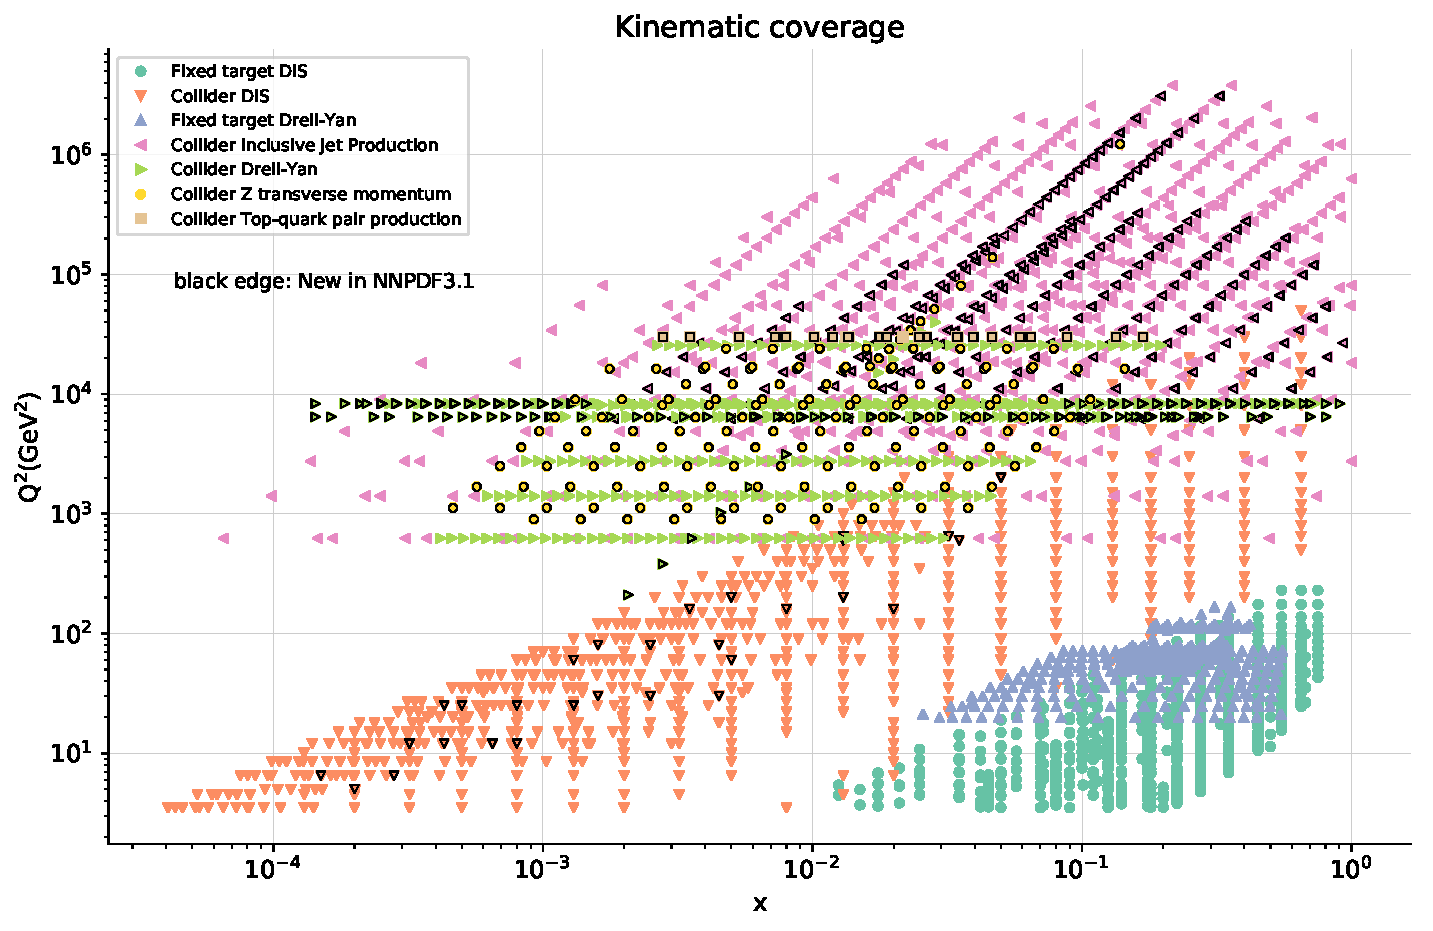
\includegraphics[scale=0.60]{plots/kinplot-report.pdf}
\caption{\small Representative kinematic coverage in the $(x,Q^2)$ plane
 of the DIS and proton-(anti)proton hard-scattering measurements that are
 used as input in a typical fit of unpolarized PDFs, 
 NNPDF3.1~\cite{Ball:2017nwa}.
 %
 Different datasets have been clustered together into families of
 related processes.
 %
 For hadronic cross-sections, leading order kinematics is assumed to map
 each experimental bin to a pair of points in the $(x,Q^2)$ plane.
 %
 Additional precise data from SLAC and Jefferson Lab exist also in the 
 bottom right corner of the $(x,Q^2)$ plane, although they were excluded from 
 the NNPDF3.1 fit by the cut on the invariant mass of the final 
 state $W^2<12.5$~GeV$^2$ adopted there.}
\label{fig:kinplot-report} 
\end{figure}
%-------------------------------------------------------------------------------

\paragraph*{State-of-the-art global PDF fits.}
%
Various collaborations provide regular updates of their global unpolarized
PDF fits.
%
The latest fits from the three main global fitting collaborations
are CT14~\cite{Dulat:2015mca}, MMHT14~\cite{Harland-Lang:2014zoa} and
NNPDF3.1~\cite{Ball:2017nwa}.
%
These fits are performed up to NNLO in the strong coupling (with central value
$\alpha_s(m_Z)=0.118$), and include data from the HERA $e^{\pm} p$ collider, 
fixed (nuclear and proton) target experiments, the Tevatron $p\overline{p}$ 
collider and the LHC. 
%
The ABMP16~\cite{Alekhin:2017kpj} set fits to a similar global data set
(although excluding jet production) but differs in its treatment of errors,
 heavy flavors and the low-$Q^2$ and large-$x$ regions.
%
The HERAPDF2.0~\cite{Abramowicz:2015mha} set fits to the final combined HERA 
Run I + II data set only, with the aim of determining the PDFs from a 
completely consistent DIS data sample; in $x$ regions that are less constrained 
by HERA data, the uncertainties can be quite large.
%
The CJ15~\cite{Accardi:2016qay} NLO set focuses on constraining the PDFs at 
higher $x$ by lowering $Q^2$ and $W^2$ cuts in DIS.
%
This greatly increases the amount of available data, but requires additional 
modeling of power-like ${\cal O}(1/Q^2)$ corrections.

The features of each PDF set have been discussed in detail in 
Refs.~\cite{Butterworth:2015oua,Accardi:2016ndt}, including the 
dataset, the fitting methodology, the theoretical details of the 
corresponding QCD analyses, and, most importantly, the uncertainties
coming from each of these aspects.

In Fig.~\ref{fig:globalfits}
we present a snapshot of the current understanding
of the proton structure in the global PDF fitting framework.
%
We compare the CT14, MMHT2014
and NNPDF3.1 NNLO PDF sets at $Q=100$~GeV, normalized
to the central value of the last.
%
From top to bottom and from left to right we show the
$u$, $\bar{d}$ and $s$ quark PDFs and the gluon PDF.
%
The error bands indicate the 68\%-confidence level (CL) PDF uncertainties
associated with each set, computed with the corresponding master formula.
%
We observe that differences for the up quark PDF
are small, at the few percent level, but greater differences
are observed for the sea quarks, in particular
in the medium and large-$x$ region.
%
For the gluon there is reasonable agreement except in the large-$x$ region, 
where NNPDF3.1 is softer than CT14 and MMHT14.
%
Any other comparison plots between PDFs can be straightforwardly
obtained using the {\tt APFEL-Web} online plotting 
interface~\cite{Carrazza:2014gfa}.

%-------------------------------------------------------------------------------
\begin{figure}[!t]
\centering
 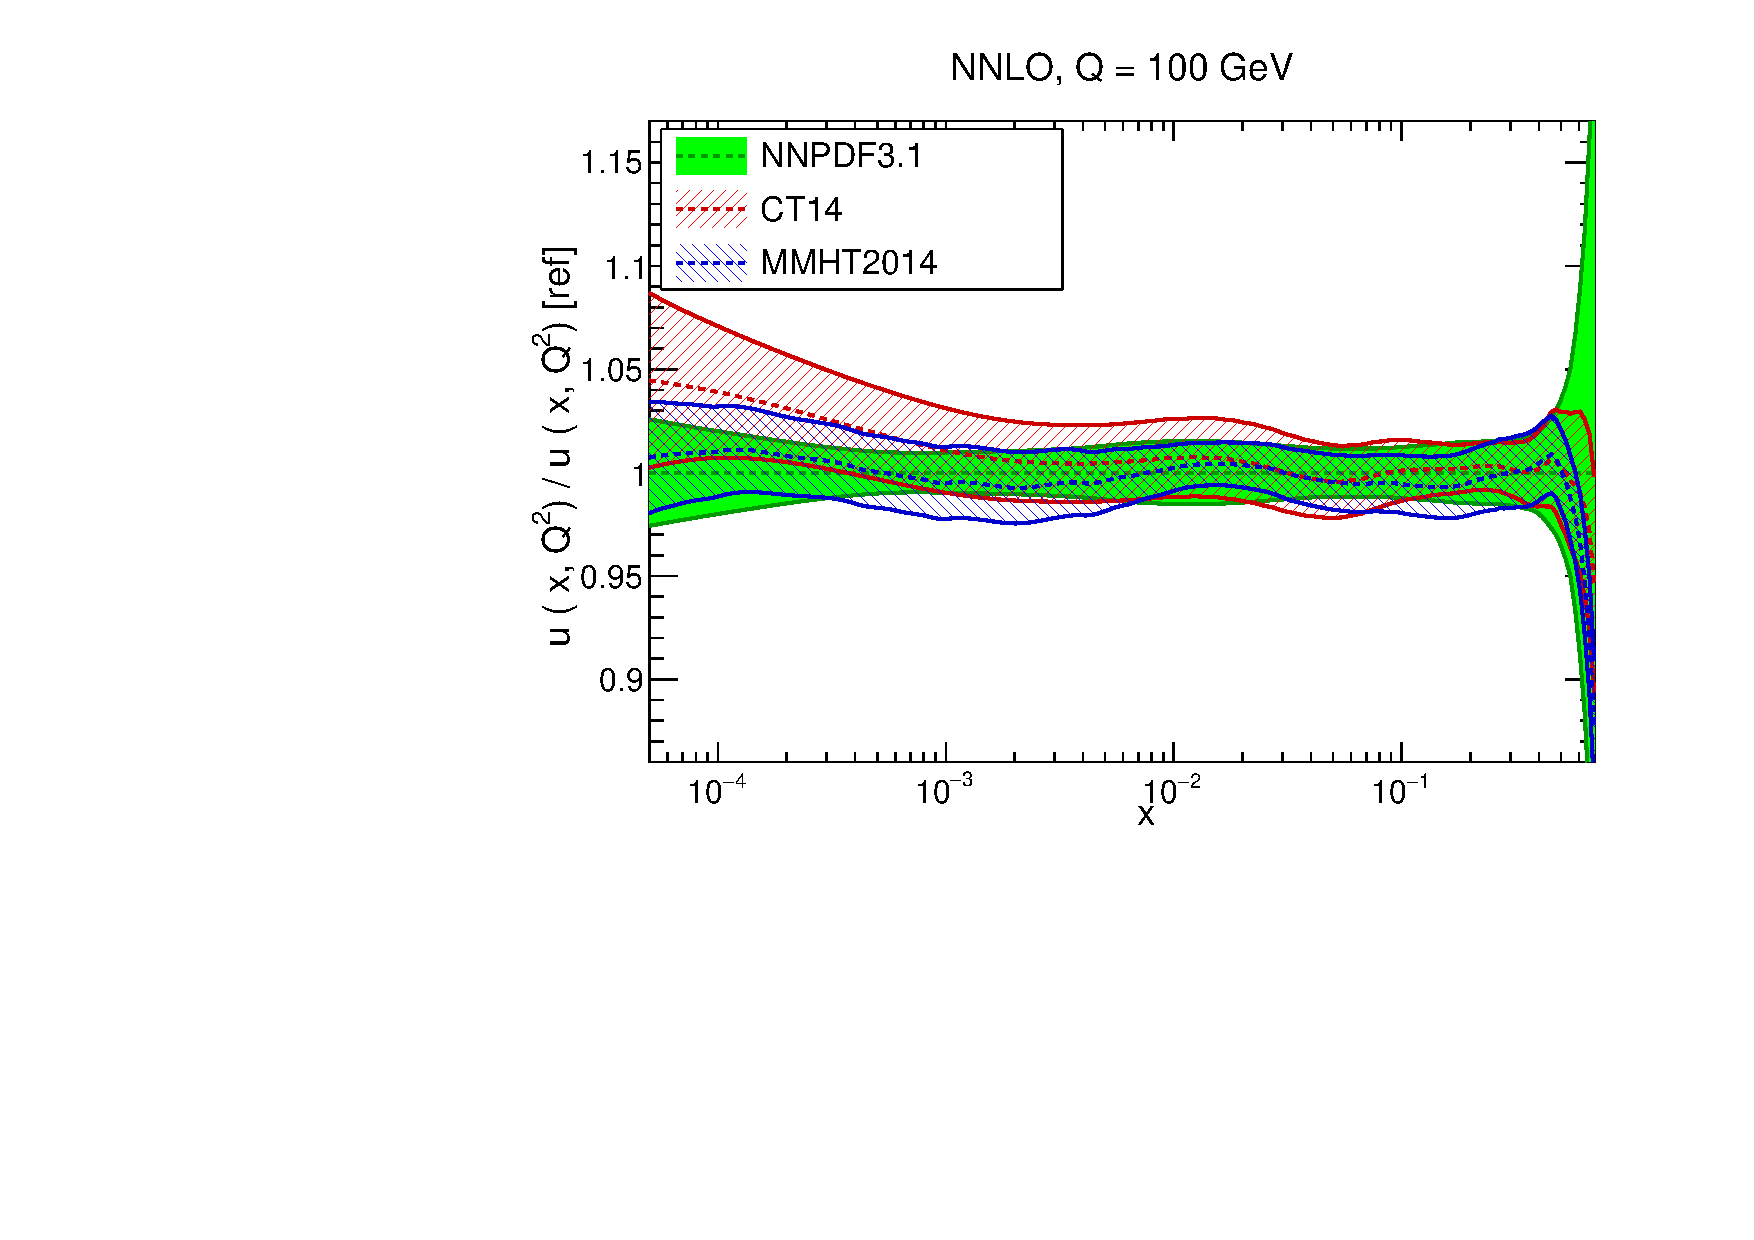
\includegraphics[scale=0.37]{plots/xu-31-nnlo-globalfits.pdf}
 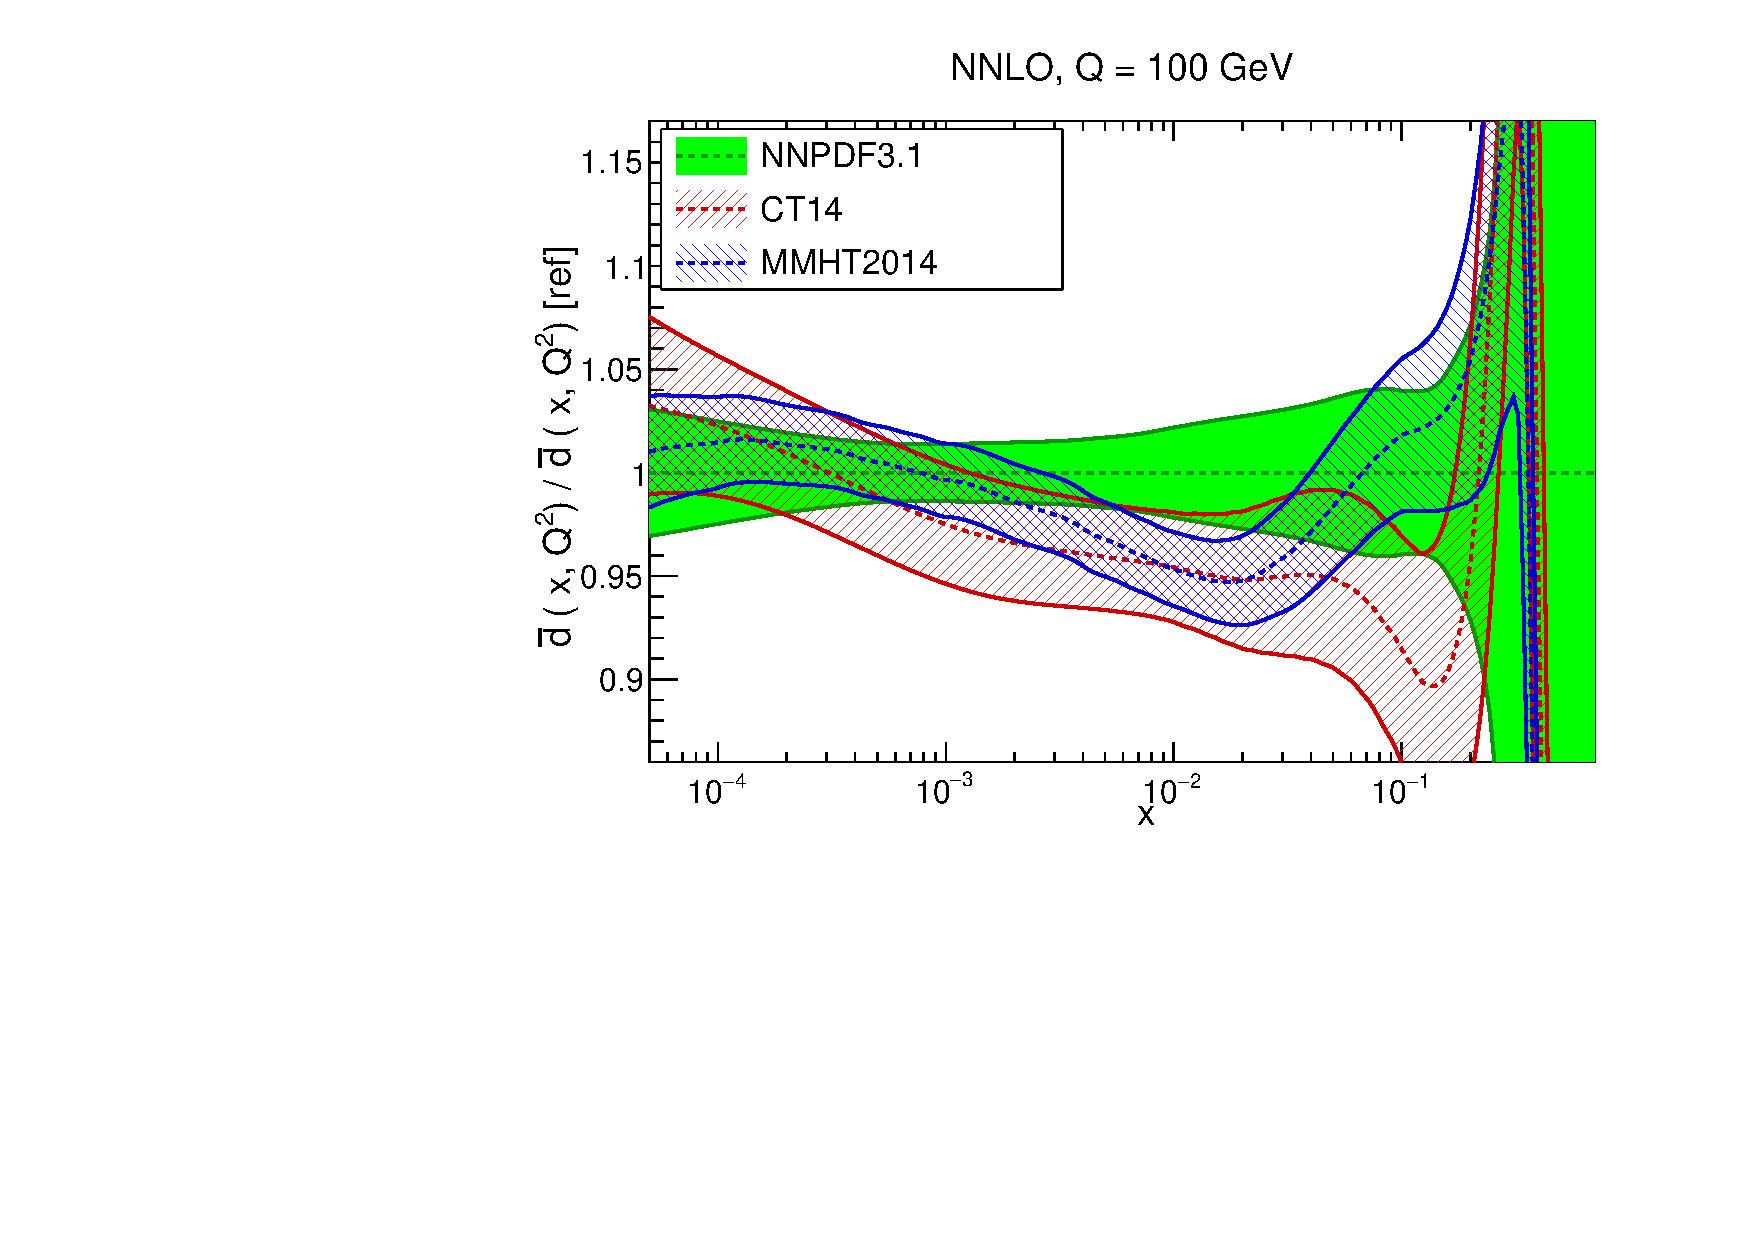
\includegraphics[scale=0.37]{plots/xdbar-31-nnlo-globalfits.pdf}\\
 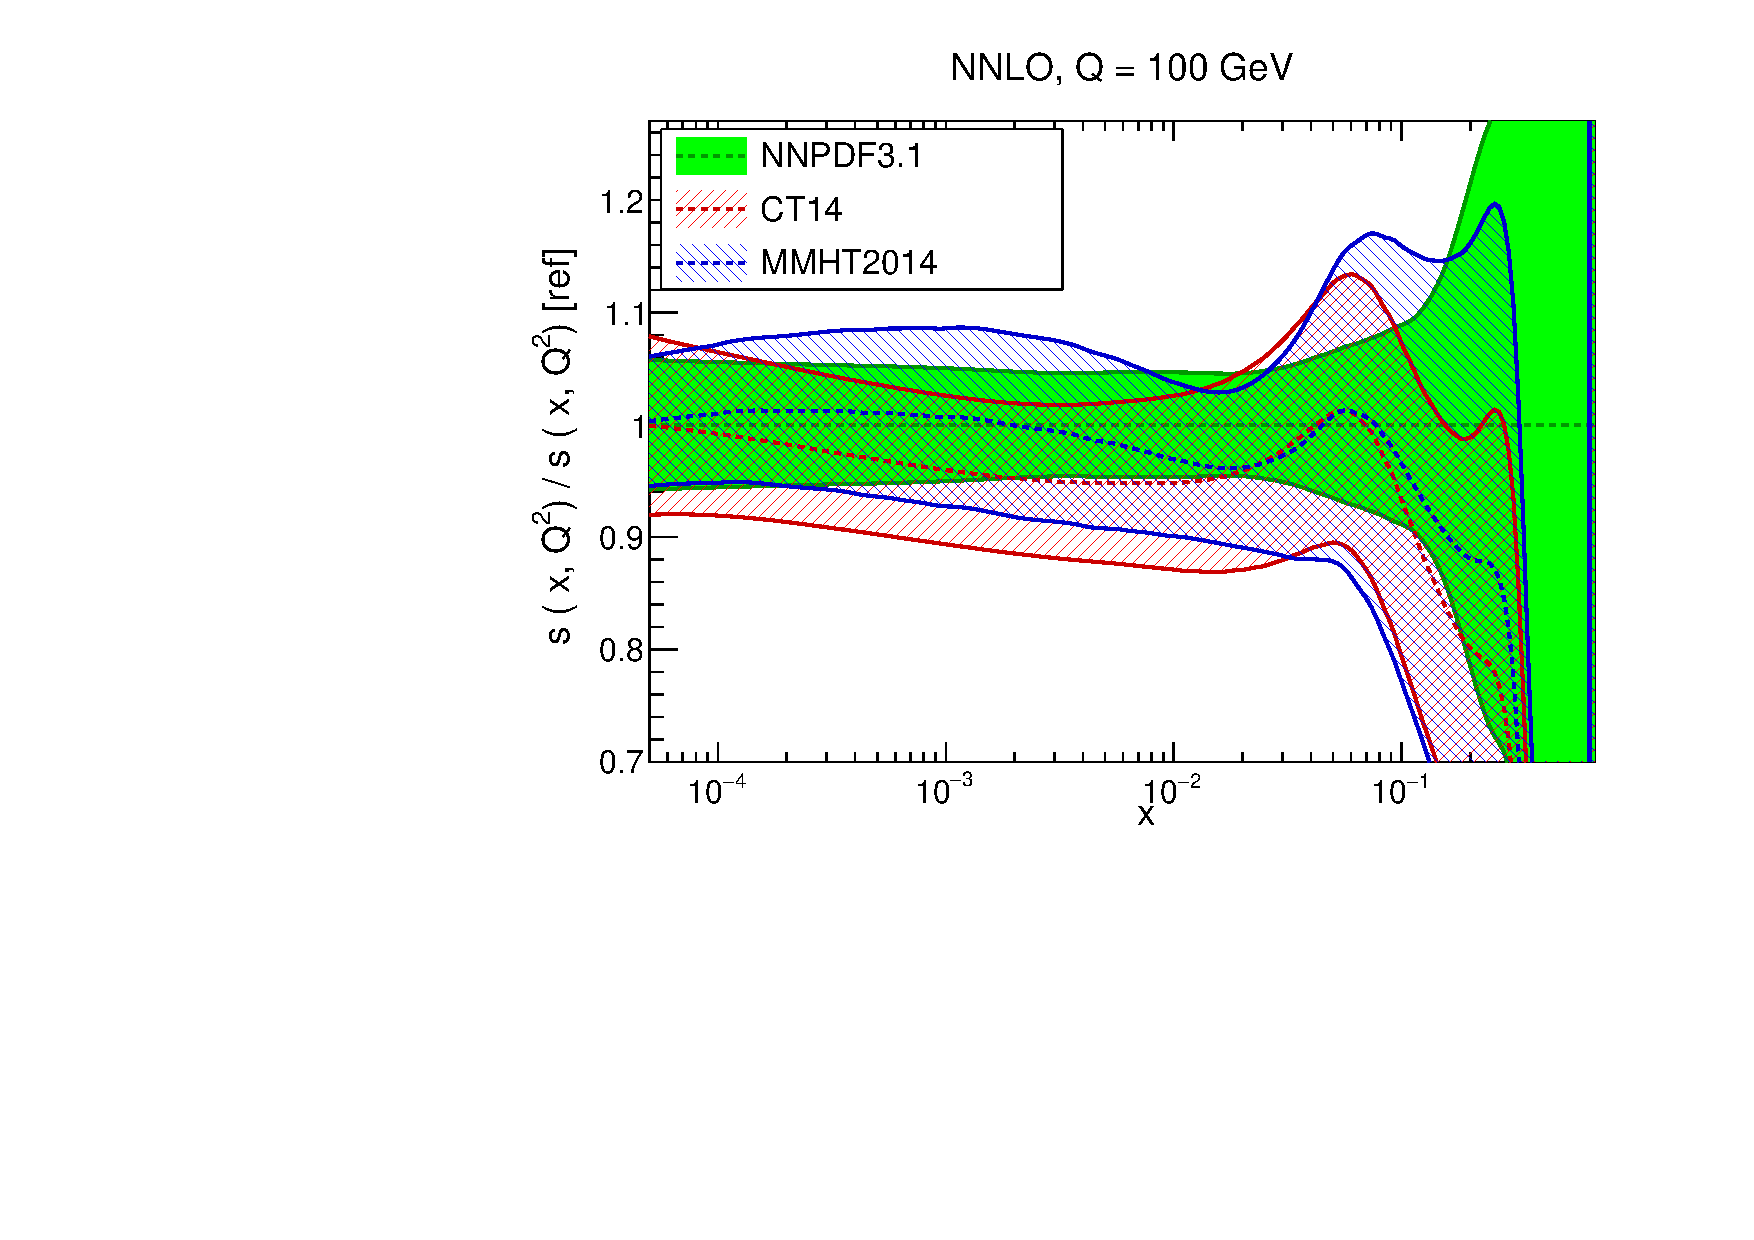
\includegraphics[scale=0.37]{plots/xs-31-nnlo-globalfits.pdf}
 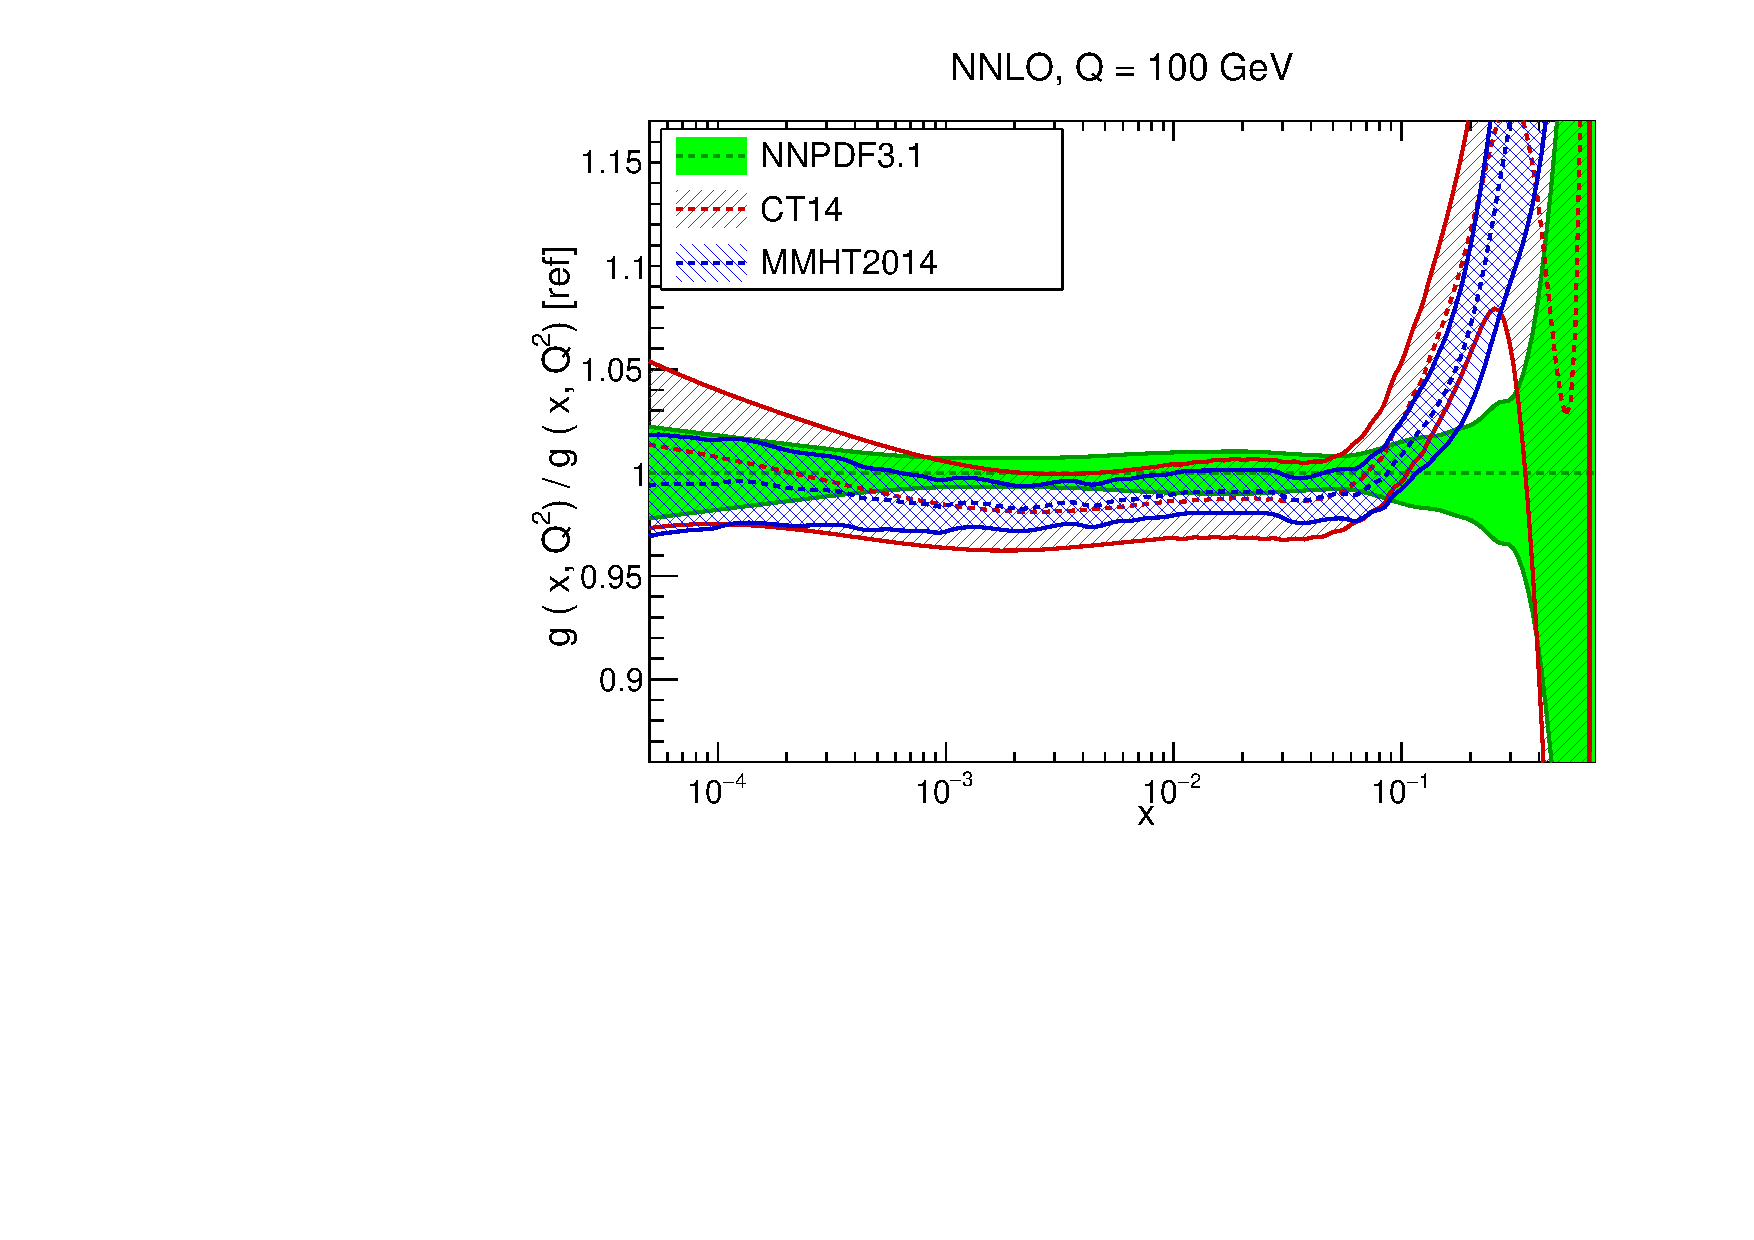
\includegraphics[scale=0.37]{plots/xg-31-nnlo-globalfits.pdf}\\
 \caption{\small Comparison between the CT14, MMHT2014
  and NNPDF3.1 NNLO PDF sets at $Q=100$~GeV, normalized
  to the central value of the latter.
  %
  From top to bottom and from left to right we show the
  $u$, $\bar{d}$ and $s$ quark PDFs as well as the gluon.
  %
  The error bands indicate the 1-$\sigma$ PDF uncertainties
  associated with each set.
  %
  These PDF comparison plots have been produced using the
  {\tt APFEL-Web} online plotting interface~\cite{Carrazza:2014gfa}.
    \label{fig:globalfits}
  }
\end{figure}
%-------------------------------------------------------------------------------

In addition to these latest versions of the global PDF fits,
there has recently been a significant development of techniques aiming
to construct combined PDF sets that are based on
a small number of Hessian eigenvectors or MC replicas and thus
are more efficient to use in lengthy higher-order
computations or Monte Carlo simulations.
%
In particular, the PDF4LHC15 PDF sets are based on the
combination of the CT14, MMHT14 and NNPDF3.1 NNLO PDF sets,
subsequently reduced to a small number of eigenvectors
(replicas) using the META-PDF~\cite{Gao:2013bia}
and MC2H~\cite{Carrazza:2015aoa}
(CMC~\cite{Carrazza:2015hva}) compression algorithms.
%
In this respect, Specialized Minimal PDF sets~\cite{Carrazza:2016htc}
(SM-PDFs) have also
been advocated, which
are tailored to specific physical processes and are based
on a minimal number of Hessian eigenvectors.
%
%The PDF4LHC15 sets provide a suitable representative for the expectations
%from the global QCD analysis point of view, and as such will be used
%in the benchmark comparisons of the next section.

The PDF4LHC15 NLO set~\cite{Butterworth:2015oua} is displayed in 
Fig.~\ref{fig:nnlopdfs} at $\mu^2=Q^2=4~{\rm GeV}^2$ and at
$\mu^2=Q^2=10^2~{\rm GeV}^2$.
%
Specifically, we show the $u_v=u-\bar{u}$ and $d_v=d-\bar{d}$ valence 
combinations, the $\bar{u}$, $\bar{d}$, $s$ and $c$ sea quark PDFs, 
and the gluon (divided by a factor 10).
%
The evolution between $Q^2=4$~GeV$^2$ to $Q^2=10^2$~GeV$^2$ is completely
determined by the solution of the DGLAP evolution equations.
%
The shape of the $u_v~(u^{-})$ and $d_v~(d^{-})$ valence quark combinations
reflects the constraints from the valence sum rules 
Eq.~\eqref{eq:valencesumrules}.
%
At small $x$, there is a rapid growth of the gluon and the sea quark PDFs, 
implying that the higher the collision center-of-mass energy $\sqrt{s}$, 
the more important gluon- and sea-quark-initiated processes become.
%
The bands in Fig.~\ref{fig:nnlopdfs} represent the 68\% CL PDF uncertainties.

%-------------------------------------------------------------------------------
\begin{figure}[!t]
\centering
  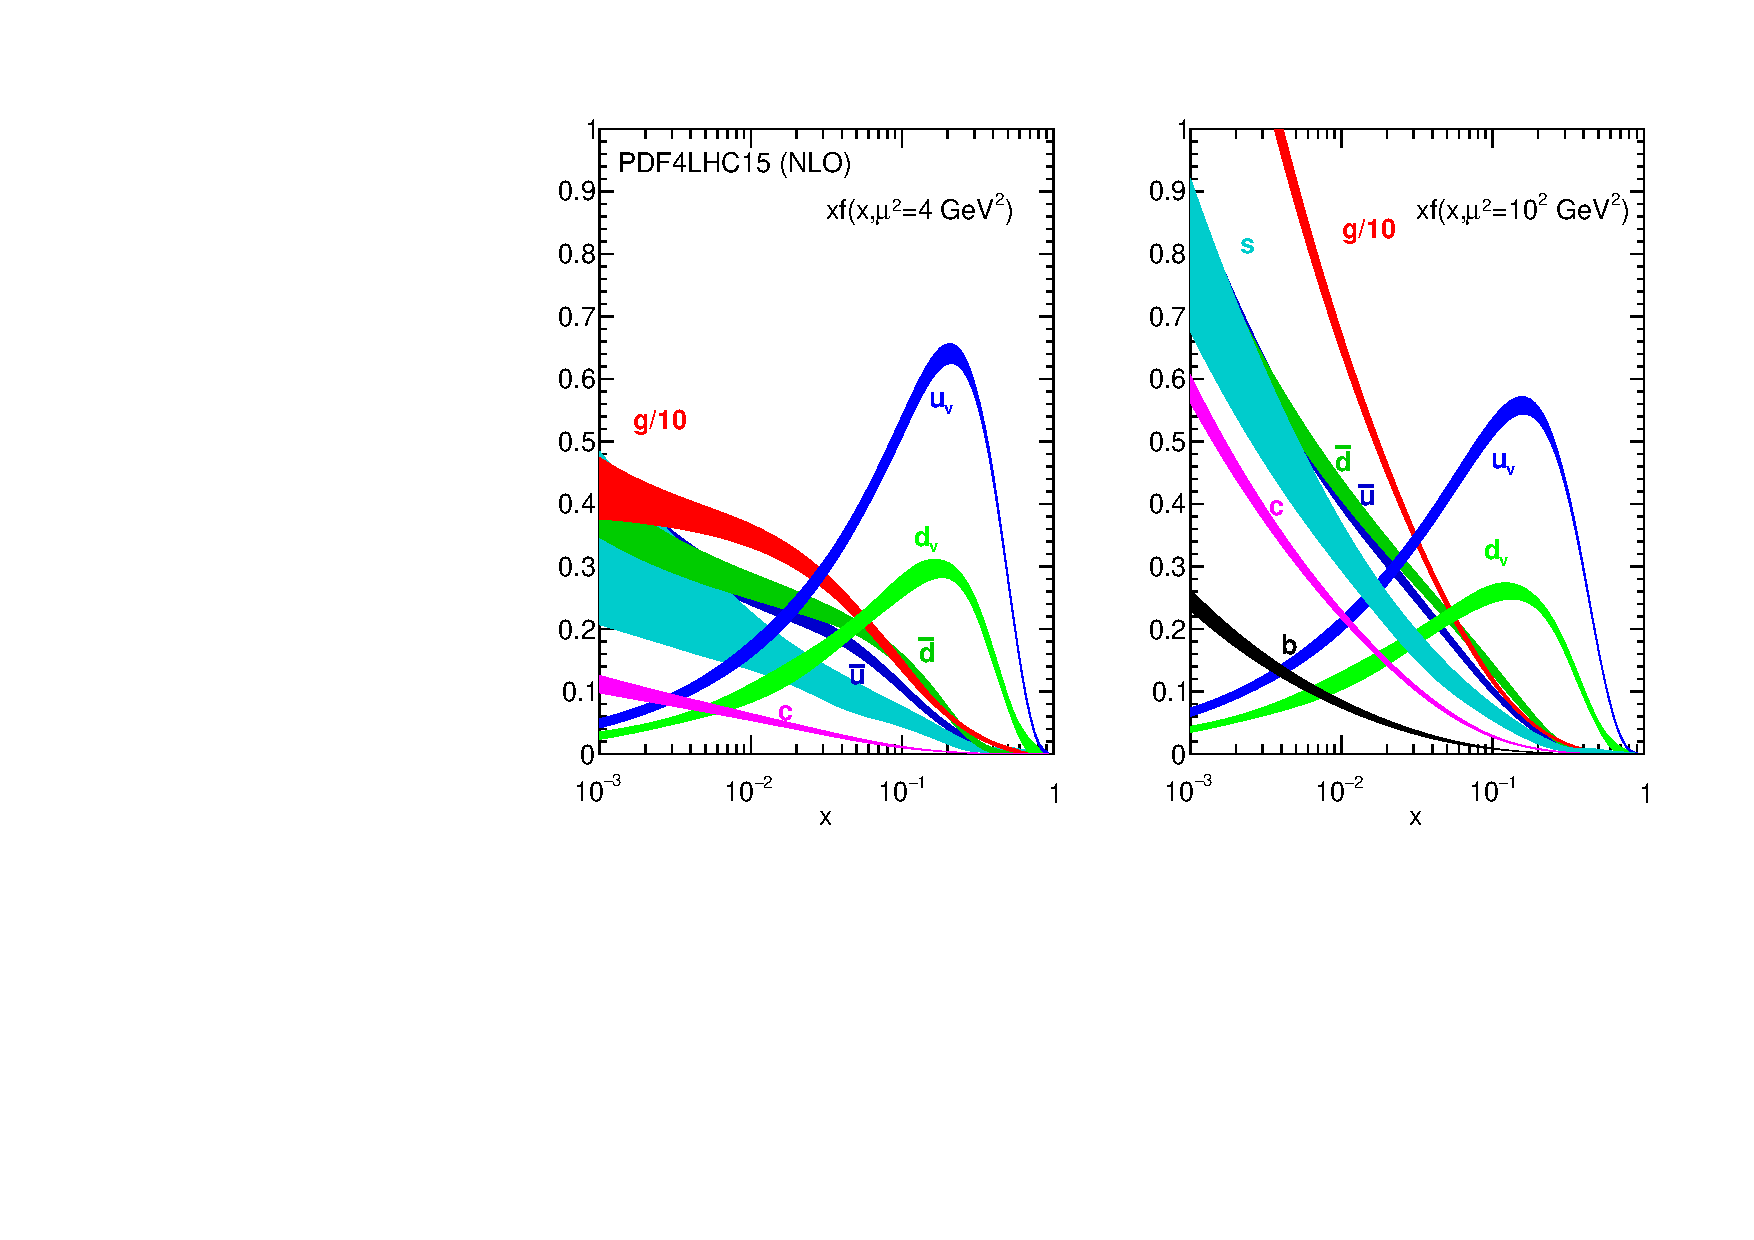
\includegraphics[scale=0.8]{plots/PDF4LHC15.pdf}\\
  \caption{\small The PDF4LHC15 NLO PDFs at a low scale
    $\mu^2=Q^2=4~{\rm GeV}^2$ (left plot) and at 
    $\mu^2=Q^2=10^2~{\rm GeV}^2$ (right plot) as a function of $x$.
    %
    We show the $u_v$ and $d_v$ valence combinations, the $\bar{u}$,
    $\bar{d}$, $s$ and $c$ sea quark PDFs, and the gluon (note that
    the latter is divided by a factor 10).
    \label{fig:nnlopdfs}
  }
\end{figure}
%-------------------------------------------------------------------------------

We strongly encourage the community to use the most recent versions
of global PDF fits when comparing with existing or new
lattice QCD calculations.
%
Comparing with deprecated sets, based on obsolete methodology
and in many cases experimental data that have been
superseded, should always be avoided.

\subsubsection{Polarized PDFs}
\label{sec:polPDFs}

\paragraph*{Theoretical features.}

The dependence on the momentum fraction $x$, fixed by nonperturbative QCD 
dynamics, should satisfy some theoretical constraints.
%
First, PDFs must lead to positive cross-sections.
At leading order (LO), this implies that polarized 
PDFs are bounded by their unpolarized counterparts\footnote{Beyond LO, more 
complicated relations hold~\cite{Altarelli:1998gn}; however they have little
effect on PDFs.}, $|\Delta f(x,\mu^2)|\leq f(x,\mu^2)$~\cite{Altarelli:1998gn}.
%
Second, PDFs must be integrable: this corresponds to the assumption 
that the nucleon matrix element of the axial current for each flavor is finite.
%
Third, SU(2) and SU(3) flavor symmetry, if assumed to be exact, imply that 
the zeroth moments of the nonsinglet $\mathcal{C}$-even PDF combinations,
$\Delta T_3=\Delta u^+ -\Delta d^+$ and 
$\Delta T_8 = \Delta u^+ +\Delta d^+ -2\Delta s^+$ 
(where $\Delta q^+=\Delta q+\Delta\bar{q}$, $q=u,d,s$), are respectively
related to the baryon octet $\beta$-decay constants, whose 
measured values are~\cite{Olive:2016xmw}
\begin{align}
 g_A  = a_3
 & =
 \int_0^1 dx \Delta T_3 (x,\mu^2)
 = \langle 1\rangle_{\Delta u^+} - \langle 1\rangle_{\Delta d^+}  = 1.2723 \pm 0.0023\,,
 \label{eq:a3}
 \\
 a_8
 & =
 \int_0^1 dx \Delta T_8 (x,\mu^2)
 = \langle 1 \rangle_{\Delta u^+} + \langle 1 \rangle_{\Delta d^+} -2\,\langle 1 \rangle_{\Delta s^+} 
 =0.585  \pm 0.025
 \,.
\label{eq:decayconst}
\end{align}
%
Fairly significant violations of SU(3) symmetry are advocated
in the literature (see {\it e.g.} Ref.~\cite{Cabibbo:2003cu} for a review). 
%
In this case, an uncertainty on the octet axial charge, which could be as 
large as 30\% of the experimental value of $a_8$ in Eq.~\eqref{eq:decayconst}, 
see Ref.~\cite{FloresMendieta:1998ii}. 

\paragraph*{Experimental data.}
The bulk of the experimental information on polarized PDFs comes from 
neutral-current (photon exchange) inclusive and semi-inclusive deep-inelastic
scattering (DIS and SIDIS) with charged lepton beams and nuclear targets. 
%
As photon scattering does not distinguish quarks and antiquarks, inclusive DIS 
data constrain only the total quark combinations $\Delta q^+$, 
while SIDIS data with identified pions or kaons in the final state 
constrain individual quark and antiquark flavors. 
%
In principle, both DIS and SIDIS are also sensitive to the gluon 
distribution $\Delta g$, as it directly enters the factorized expressions of
the corresponding structure functions beyond LO, and indirectly via DGLAP 
evolution.
%
In practice, the constraining power of DIS and SIDIS data on $\Delta g$ is 
rather weak because the $Q^2$ range covered by the data is limited,
especially if one restricts to the kinematic region not affected by
power-suppressed corrections and very precise data from JLab are therefore
excluded. 

Note that, in the case of SIDIS, a reliable knowledge of fragmentation 
functions (FFs) is required in the factorized expressions of the 
corresponding observables. 
%
Since FFs are nonperturbative objects on the same footing as PDFs, they are 
an additional source of uncertainty in PDF determinations, if not a bias.
%
A significant experimental and theoretical effort has been
invested in improving the independent determination of 
FFs~\cite{deFlorian:2014xna,deFlorian:2017lwf,
Hirai:2016loo,Sato:2016wqj,Bertone:2017tyb} and most recently in simultaneously 
fitting both PDFs and FFs~\cite{Ethier:2017zbq,Borsa:2017vwy}.

Besides DIS and SIDIS fixed-target data, a significant amount of data from
longitudinally polarized proton-proton collisions at the Relativistic 
Heavy Ion Collider (RHIC) has become available recently (see {\it e.g.} 
Ref.~\cite{Aschenauer:2015eha} for an overview), although in a limited range 
of momentum fractions, $0.05\lesssim x \lesssim 0.4$.
%
On the one hand, longitudinal (parity-violating) single-spin and 
(parity-conserving) double-spin asymmetries for $W^\pm$ boson production are 
sensitive to the flavor decomposition of polarized quark and antiquark 
distributions, because of the chiral nature of the weak 
interaction~\cite{Bourrely:1993dd}. 
%
On the other hand, double-spin asymmetries for jet, di-jet and $\pi^0$ 
production are directly sensitive to the gluon polarization in 
the proton, because of the dominance of gluon-gluon and quark-gluon initiated 
subprocesses in the kinematic range accessed by RHIC~\cite{Bourrely:1990pz}.

The kinematic coverage of the data that can be used to constrain polarized 
PDFs is displayed in Fig.~\ref{fig:kinEIC}.
%
A comparison with Fig.~\ref{fig:kinplot-report} makes it apparent that the
quantity of data points, their kinematic coverage and the variety of 
available hard-scattering processes are presently much more limited in the 
polarized case than in the unpolarized case.
%
Therefore, polarized PDFs can currently be determined with much less 
precision than their unpolarized counterparts and only over an $x$-range limited
to $x\gtrsim 0.005$.
%
The kinematic coverage is expected to be significantly extended in the future,
with DIS and SIDIS data from JLab-12~\cite{Dudek:2012vr} and a polarized 
high-energy Electron-Ion Collider (EIC)~\cite{Accardi:2012qut}.
%
Such an extended kinematic coverage is also displayed in Fig.~\ref{fig:kinEIC},
where it is denoted as eRHIC.

%-------------------------------------------------------------------------------
\begin{figure}[!t]
\centering
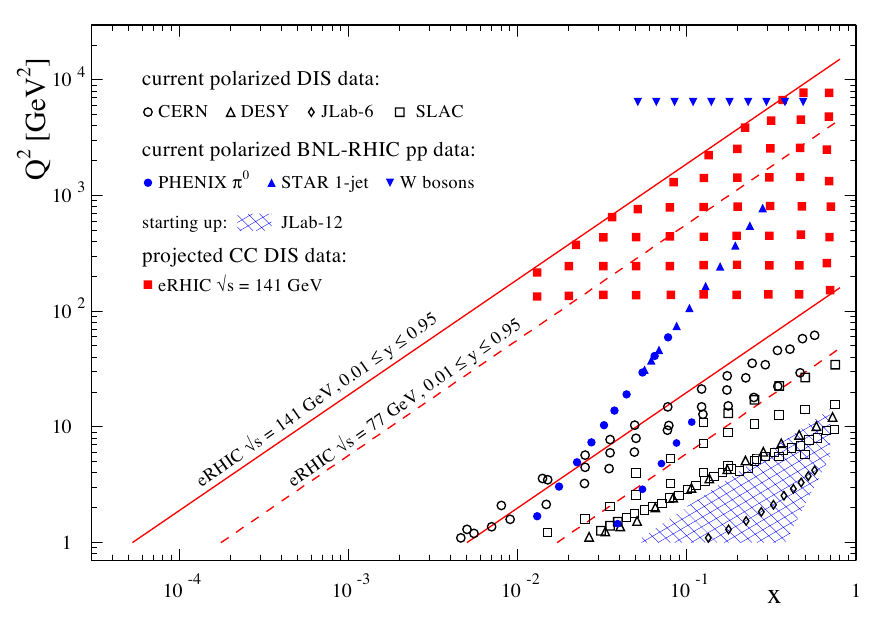
\includegraphics[width=0.9\textwidth]{plots/kinEIC}\\
\caption{\small Representative kinematic coverage, in the $(x,Q^2)$ plane,
of the (neutral current) DIS, SIDIS and proton-proton hard-scattering 
measurements that are used as input in a global polarized PDF fit.
%
The extended kinematic coverage achieved by 
JLab-12~\cite{Dudek:2012vr} and by an EIC~\cite{Accardi:2012qut}
(including projected charged-current (CC) DIS data and denoted as eRHIC) 
is also shown.
%
Figure taken from Ref.~\cite{Aschenauer:2014cki}.}
\label{fig:kinEIC}
\end{figure}
%-------------------------------------------------------------------------------

A representative illustration of polarized PDFs obtained from a global
QCD analysis, namely NNDPFpol1.1~\cite{Nocera:2014gqa}, is provided in Fig.~\ref{fig:qPDFpol}.
%
The format is the same as for the unpolarized case, Fig.~\ref{fig:nnlopdfs},
in order to ease any comparison between the two.
%
In particular, note the suppression of all polarized PDFs at small values of 
$x$, including polarized sea quark PDFs, with respect to their unpolarized 
counterparts.

%-------------------------------------------------------------------------------
\begin{figure}[!t]
\centering
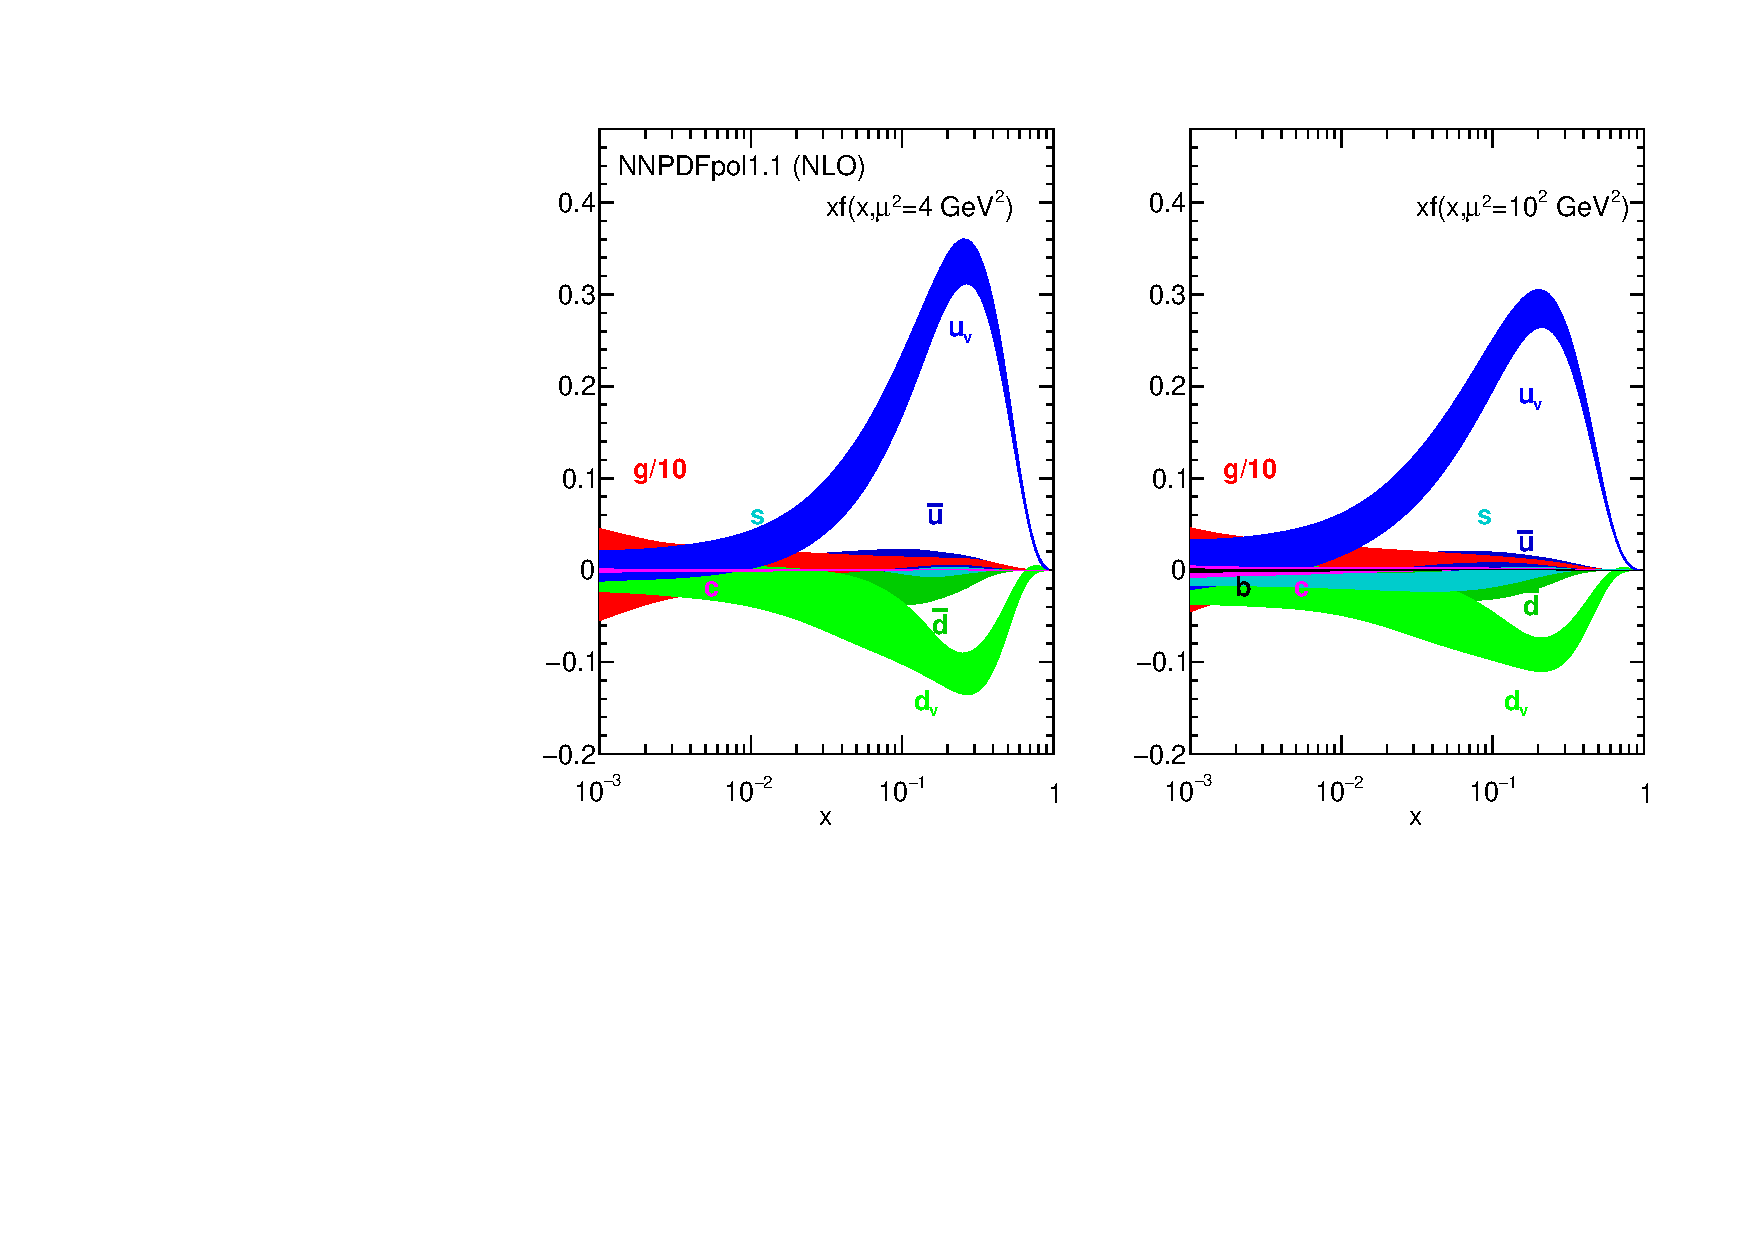
\includegraphics[scale=0.8]{plots/NNPDFpol11}\\
\caption{\small Same as Fig.~\ref{fig:nnlopdfs}, 
but for the polarized NNPDFpol1.1 NLO PDFs~\cite{Nocera:2014gqa}.}
\label{fig:qPDFpol}
\end{figure}
%-------------------------------------------------------------------------------

\paragraph{State-of-the-art global PDF fits.}

Several modern determinations of polarized PDFs of the proton (up to 
NLO\footnote{A NNLO QCD analysis of polarized PDFs based on inclusive DIS
data only was performed in Refs.~\cite{Shahri:2016uzl,Khanpour:2017cha}.
Inclusive DIS is the only polarized process for which coefficient functions
are known up to NNLO (all others are known up to NLO).} 
and mostly in the $\overline{\rm MS}$ factorization scheme) are available in 
the literature~\cite{Nocera:2014gqa,Nocera:2016xhb,deFlorian:2014yva,deFlorian:2008mr,deFlorian:2009vb,Sato:2016tuz,Leader:2010rb,Blumlein:2010rn,Bourrely:2014uha,Hirai:2008aj}. 
%
A key goal of these is to unveil the size (and uncertainty) of
$\Delta\Sigma$ and  $\Delta G$ in Eq.~\eqref{eq:moments}. 
%
The various determinations differ among each other in the data sets included 
in the analysis, in some details of the QCD analysis (like the treatment of 
higher-twist corrections) and in the procedure used to determine PDFs from the 
data (for details, see {\it e.g.} Chap.~3 in Refs.~\cite{Nocera:2014vla} 
and~\cite{Nocera:2016xhb,Jimenez-Delgado:2013sma}). 
%
The NNDPF procedure and the standard (adopted by DSSV) have 
already been outlined in Sec.~\ref{sec:genframework}. 
%
We note that DSSV has developed a method based on Mellin moments of the PDFs 
in order to efficiently incorporate NLO computations
of proton-proton cross-sections in the fitting procedure. 
%
The JAM collaboration has implemented a new approach called 
iterative Monte Carlo procedure~\cite{Sato:2016tuz,Ethier:2017zbq}
in their analyses.

The most recent analyses of polarized PDFs are DSSV14~\cite{deFlorian:2014yva}
and NNPDFpol1.1~\cite{Nocera:2014gqa}.
%
Motivated by the interest in assessing the impact of RHIC proton-proton 
data, they upgrade the corresponding previous analyses, 
DSSV08~\cite{deFlorian:2008mr,deFlorian:2009vb} and 
NNPDFpol1.0~\cite{Ball:2013lla}, with data respectively on double-spin 
asymmetries for inclusive jet production~\cite{Adamczyk:2014ozi} 
and $\pi^0$ production~\cite{Adare:2014hsq} (DSSV14\footnote{Preliminary 
RHIC results included in Ref.~\cite{deFlorian:2008mr} were replaced in
Ref.~\cite{deFlorian:2014yva} with final results.}), 
and on double-spin asymmetries for high-$p_T$ inclusive jet 
production~\cite{Adamczyk:2014ozi,Adamczyk:2012qj,Adare:2010cc} and single-spin
asymmetries for $W^\pm$ production~\cite{Adamczyk:2014xyw} (NNPDFpol1.1).
%
The new data have been included in NNPDFpol1.1 
by means of Bayesian reweighting~\cite{Ball:2010gb},
and in DSSV14 by means of a full refit.  

Overall, both the DSSV14 and NNPDFpol1.1 PDF determinations are 
state-of-the-art in the inclusion of the available experimental information. 
%
The data sets in the two analyses differ between each other only in
fixed-target SIDIS and RHIC $\pi^0$ production measurements, included in 
DSSV14, but not in NNPDFpol1.1. 
%
The information brought in by these data is complementary to that provided by 
RHIC $W^\pm$ production and inclusive jet production data respectively,
although fraught with larger theoretical uncertainties related to fragmentation.

%------------------------------------------------------------------------------
\begin{figure}[!t]
\centering
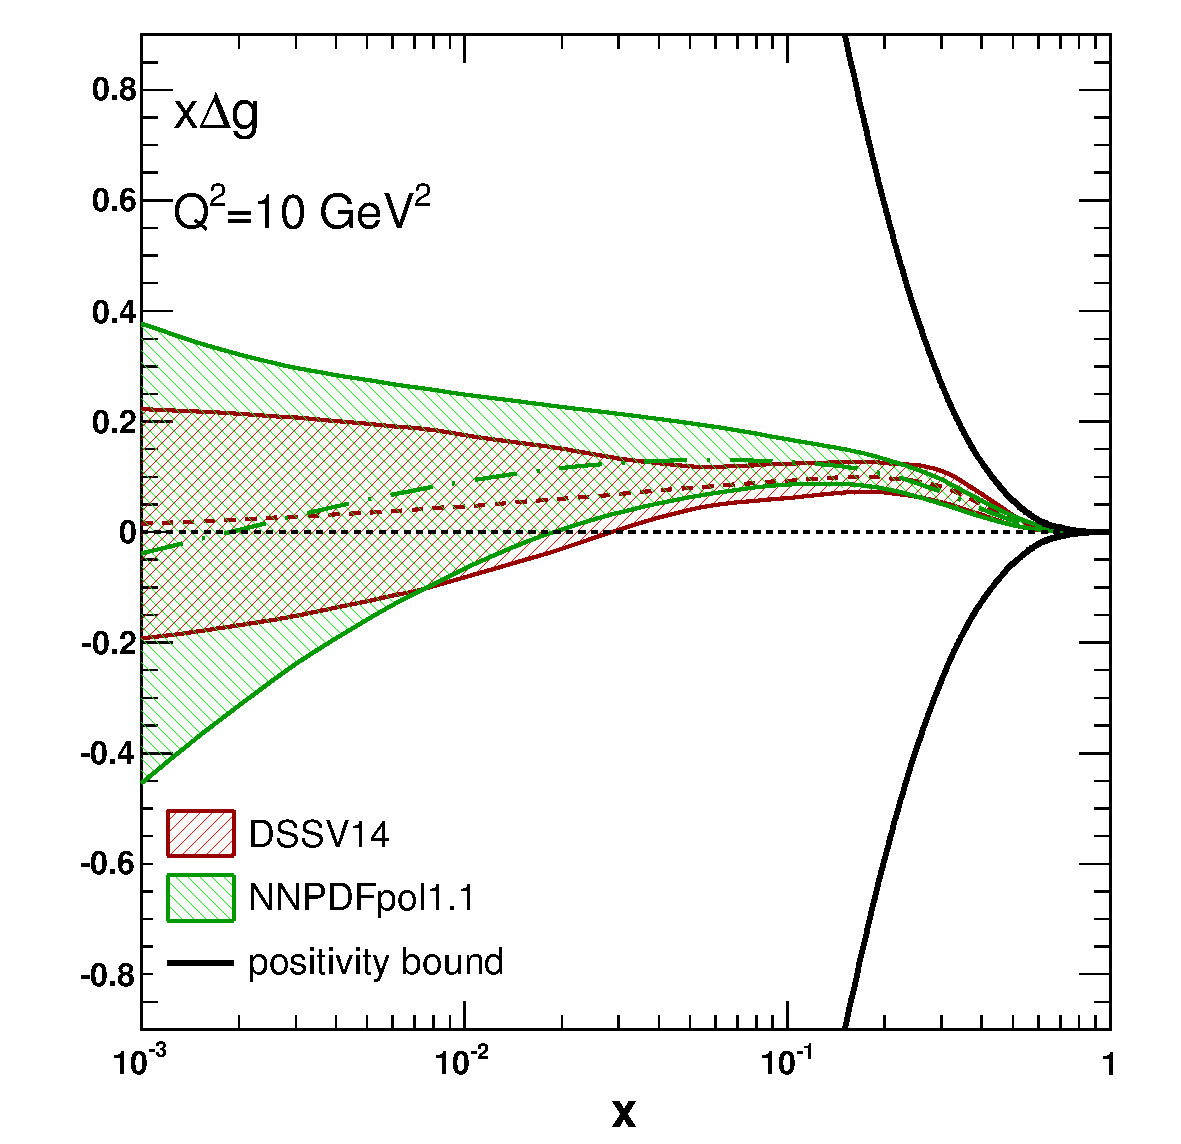
\includegraphics[scale=0.33,clip=true,trim= 0 -1.3cm 0 0]{plots/gluoncomp}
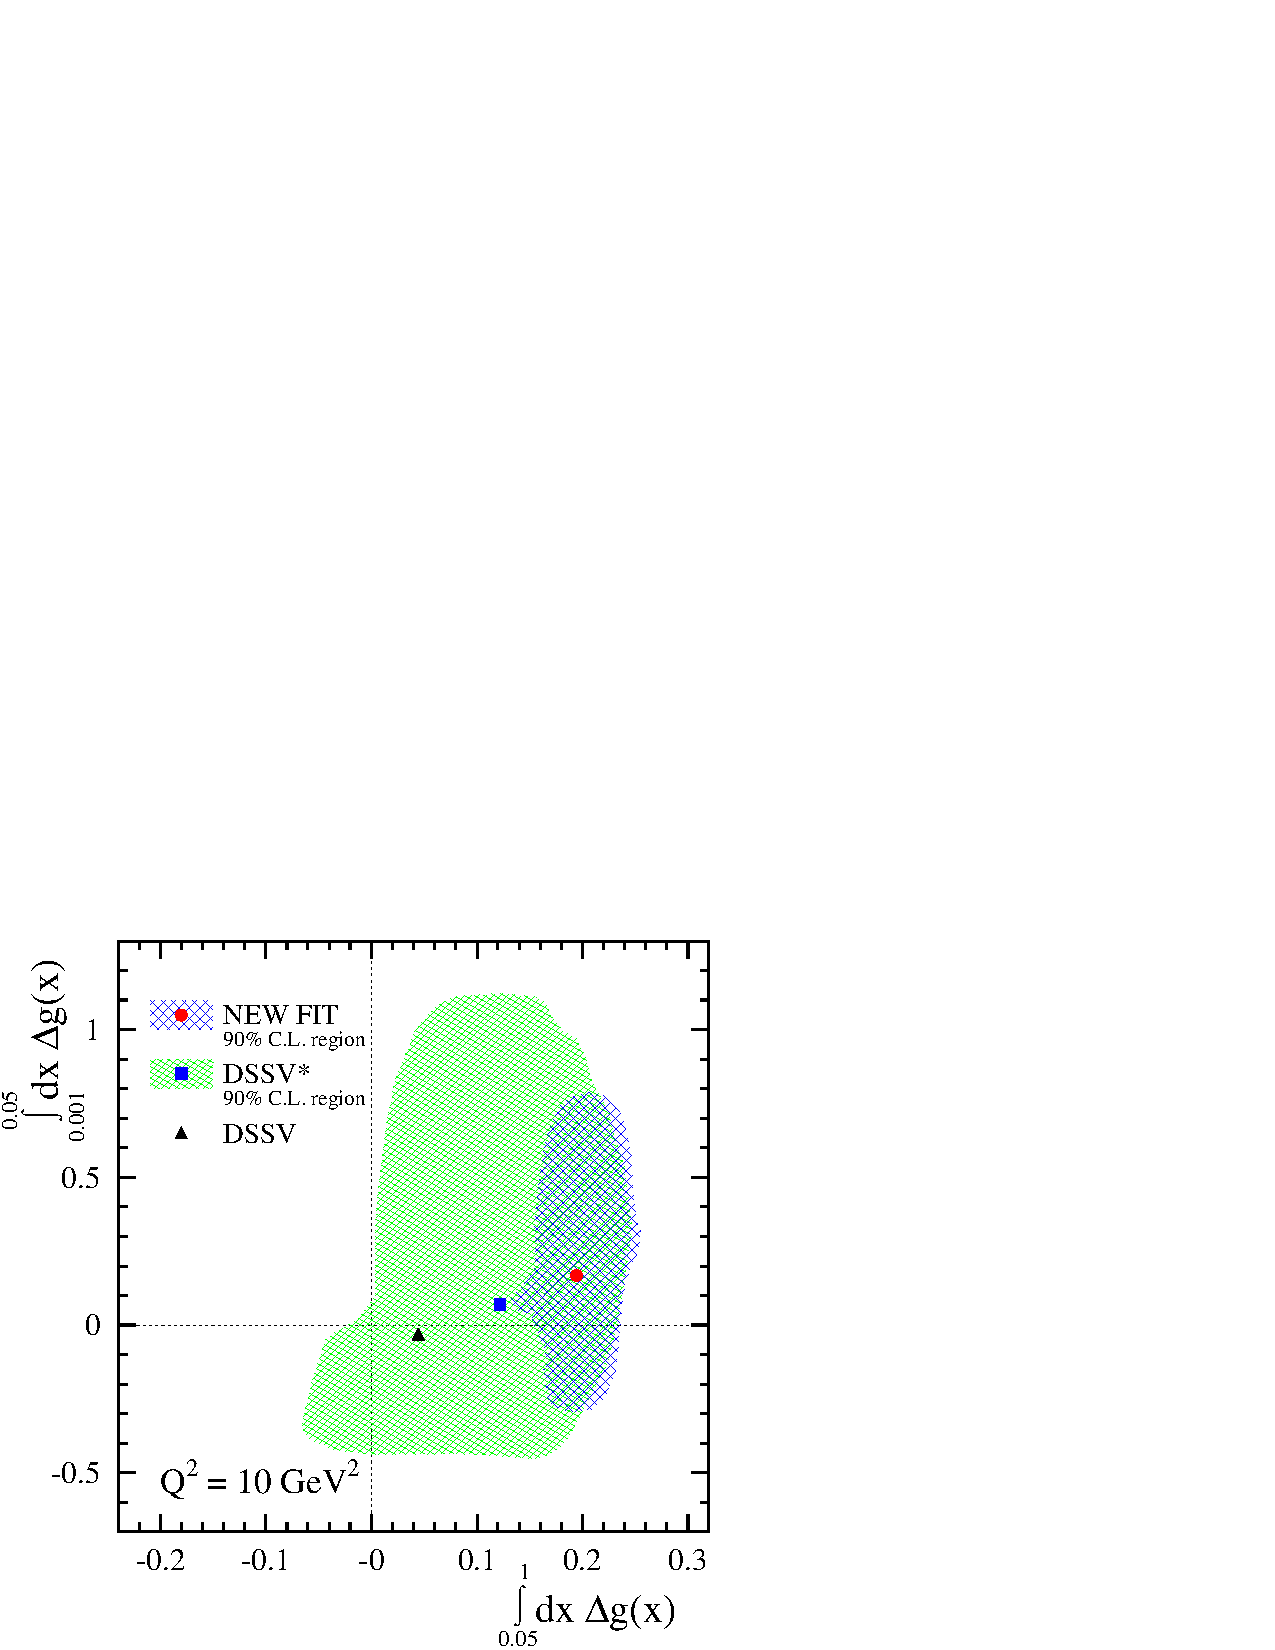
\includegraphics[scale=0.555,clip=true,trim=0 0 7cm 15cm]{plots/correlation_getot.pdf}\\
\caption{\small (Left) The polarized gluon momentum distribution  
$x\Delta g$ from the DSSV14 (with $90\%$ C.L. uncertainty band)
and NNPDFpol1.1 PDF sets at $Q^2=10$~GeV$^2$. The NNPDF3.1 positivity
bound is also shown.
(Right) $90\%$ C.L.\ areas in the plane spanned by the truncated moments of
$\Delta g$ computed for $0.05\leq x\leq 1$ and $0.001\leq x\leq 0.05$ at $Q^2=10\,\mathrm{GeV}^2$~\cite{deFlorian:2014yva}.}
\label{fig:RHICpdfs}
\end{figure}
%------------------------------------------------------------------------------

The effect of RHIC data on the polarized PDFs of the proton is twofold:
\begin{itemize}

\item The 2009 STAR and PHENIX data sets on jet and $\pi^0$ 
production~\cite{Adamczyk:2014ozi,Adare:2014hsq}, included in DSSV14
and NNPDFpol1.1, provide the first evidence
of a sizable positive gluon polarization in the proton. 
%
A comparison of the gluon PDF in the two PDF sets is displayed in 
Fig.~\ref{fig:RHICpdfs} (left panel). 
%
Comparable results, both central values and uncertainties, are found in the 
$x$ region covered by RHIC data. 
%
The agreement between the two analyses is optimal in the
range $0.08\leq x \leq 0.2$, where the dominant experimental information comes
from jet data; a slightly smaller central value is found in the DSSV14 
analysis, in comparison to NNPDFpol1.1, in the range 
$0.05\leq x \leq 0.08$, where the dominant experimental information comes from 
$\pi^0$ production data. 
%
Indeed, these are included in DSSV14 but are not in NNPDFpol1.1. 
%
Nevertheless, best fits lie well within each other's error
bands, though NNPDFpol1.1 uncertainties tend to be larger than DSSV14
uncertainties outside the region covered by RHIC data.
%
Very consistent values of the zeroth moment of $\Delta g$, 
Eq.~\eqref{eq:moments}, truncated over the interval $0.05\leq x \leq 1$, are 
found: at $Q^2=10$~GeV$^2$, this is $0.20^{+0.06}_{-0.07}$ for 
DSSV14~\cite{deFlorian:2014yva}, and $0.23\pm 0.06$ for 
NNPDFpol1.1~\cite{Nocera:2014gqa}. The right plot in Fig.~\ref{fig:RHICpdfs} 
shows the corresponding DSSV14 result as an example; the impact of the RHIC
data is clearly visible. 

\item The 2012 STAR data sets on $W$ production~\cite{Adamczyk:2014xyw}, 
included in NNPDFpol1.1, provide evidence of a positive 
$\Delta\bar{u}$ distribution 
and a negative $\Delta\bar{d}$ distribution, with 
$|\Delta\bar{d}|>|\Delta\bar{u}|$~\cite{Nocera:2014gqa}.
% 
The size of the flavor symmetry breaking for polarized sea quarks is 
quantified by the asymmetry $\Delta\bar{u}-\Delta\bar{d}$, which,
in the NNPDFpol1.1 analysis, turn out to be roughly as large as its 
unpolarized counterpart (in absolute value)~\cite{Ball:2017nwa}, 
though much more uncertain~\cite{Nocera:2014rea}. 
%
Even within this uncertainty, polarized and unpolarized light sea quark 
asymmetries show opposite signs, with the polarized one being clearly positive. 
% 
This trend is also found from analysis of the polarized SIDIS data, 
as revealed by the DSSV08 parton set. 
%
This result may discriminate among various models of nucleon structure, 
see~\cite{Nocera:2014rea} and references therein. 
%Fig.~\ref{fig:RHICpdfs1}: 
%specifically, some meson-cloud (MC) models are disfavored, while a more 
%accurate experimental information is needed to establish whether 
%chiral quark-soliton (CQS), Pauli-blocking (PB) or statistical (ST)
%models are preferred (all these models are described in Ref.~\cite{Chang:2014jba}).

\end{itemize}

%------------------------------------------------------------------------------
%\begin{figure}[!h]
%\centering
%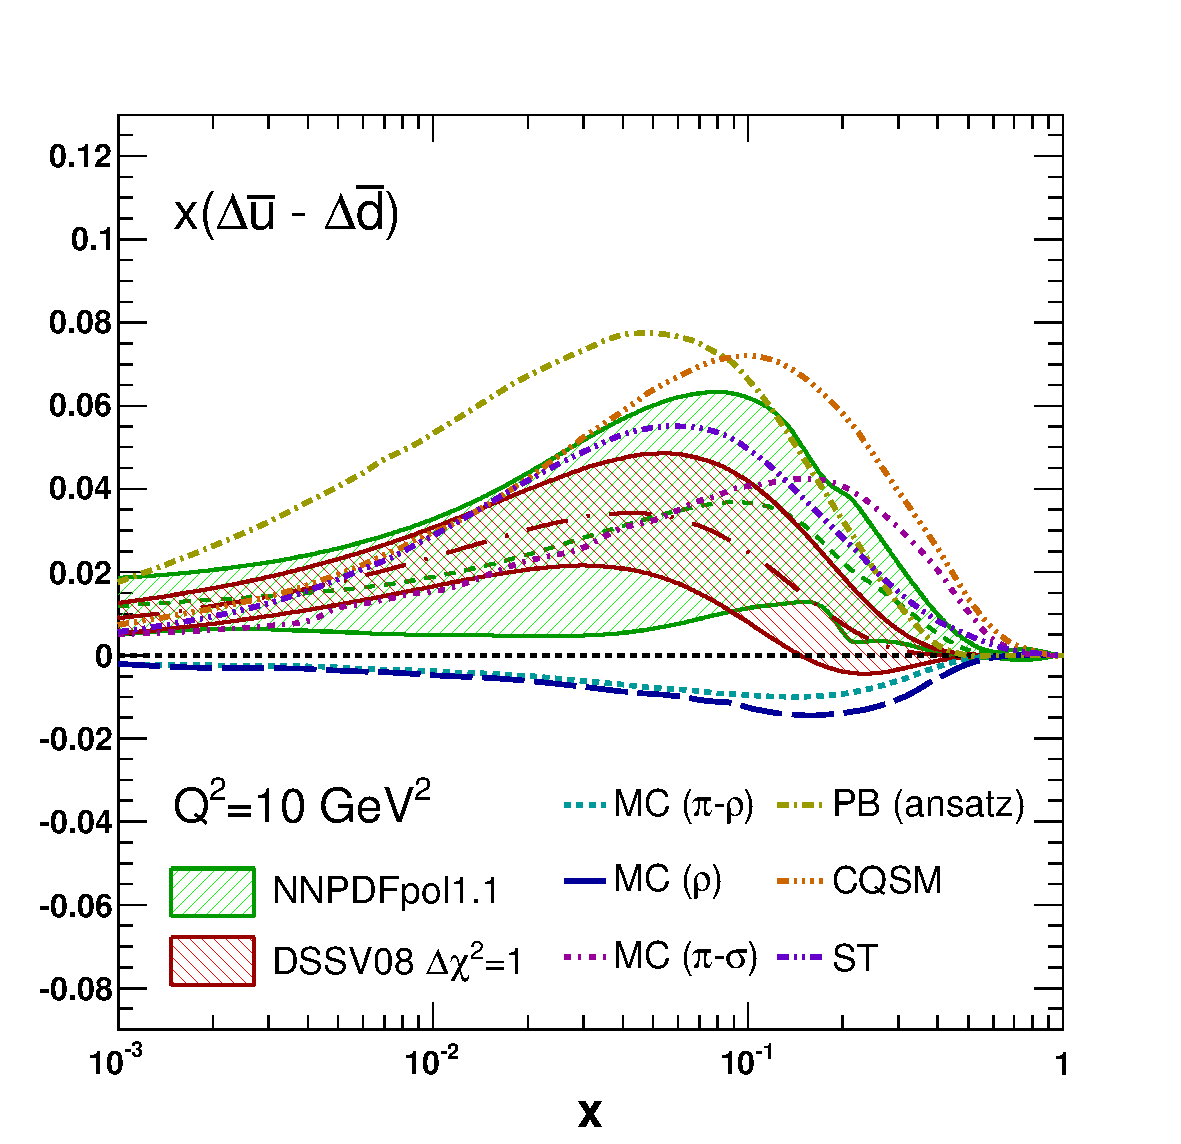
\includegraphics[scale=0.35]{plots/asysea_2}\\
%\caption{\small The polarized light sea quark asymmetry 
%$x(\Delta\bar{u}-\Delta\bar{d})$ from the NNPDFpol1.1 and 
%DSSV08 PDF sets at $Q^2=10$~GeV$^2$, compared to expectations from 
%various models of nucleon structure~\cite{Chang:2014jba}.}
%\label{fig:RHICpdfs1}
%\end{figure}
%------------------------------------------------------------------------------

\paragraph{Open issues.}

Despite the achievements described above, the polarized PDFs presently cannot 
be determined in a global QCD analysis with the same accuracy as their 
unpolarized counterparts.
%
The experimental data are confined to a relatively narrow range of 
$x$ and $Q^2$.
%
As a consequence, the size of the contributions of quarks, antiquarks and 
gluons to the nucleon spin, as quantified by their zeroth moments, 
Eq.~\eqref{eq:moments}, are still affected by large uncertainties. 
%
These come predominantly from the extrapolation into the small-$x$ region 
($x\lesssim 10^{-3}$). 
%
Here potential modifications in the PDF shape induced by small-$x$ 
evolution~\cite{Bartels:1995iu,Bartels:1996wc,Kovchegov:2015pbl,
Kovchegov:2016weo,Kovchegov:2016zex,Kovchegov:2017jxc,Kovchegov:2017lsr} 
could arise, which presently cannot be tested.
%
Significant uncertainties also affect the PDFs in the large-$x$ 
{\it valence} region ($x\gtrsim 0.7$). 
%
This regime is less relevant for the determination of the PDF moments, but it 
is important for comparisons to nonperturbative models of nucleon structure, 
especially in terms of ratios of light-quark polarized to unpolarized PDFs 
(for a comparison between large-$x$ PDFs 
and model predictions, see Ref.~\cite{Nocera:2014uea}).
%
Finally, the small lever arm of the data in $Q^2$ is a serious limiting factor 
in the determination of $\Delta g$ via evolution, unless the data at low $Q^2$
and large $x$ are included in the fit and carefully analyzed.
%
This requires an appropriate treatment of power-suppressed corrections and 
possibly a minimization methodology which can iteratively focus on a region 
in parameter space where constraints are not too strong, as done in the 
JAM15 analysis~\cite{Sato:2016tuz}. 

The determination of the total polarized strange distribution $\Delta s^+$ is 
also particularly delicate.
%
Inclusive DIS data, together with nonsinglet axial couplings, 
Eq.~\eqref{eq:decayconst}, and kaon SIDIS data provide the sole available 
constraint on $\Delta s^+$.
%
A sizable negative $\Delta s^+$ is found 
consistently in all analyses based on inclusive DIS data only, as a result 
of the constraint from hyperon decays that is usually adopted. 
%
However, the shape of $\Delta s^+$ may change significantly in analyses that also include
SIDIS data. Typically SIDIS data lead to a trend for $\Delta s^+$ to be
small or even slightly positive in the medium $x$-range, although this depends 
also on the set of kaon FFs used to compute
the corresponding observables~\cite{Leader:2011tm}.  
%
The recent study in Ref.~\cite{Ethier:2017zbq} sheds some light on this issue
by performing a simultaneous determination of polarized PDFs and unpolarized 
FFs using DIS, SIDIS and single-inclusive annihilation data.
%
In order to avoid biasing the determination of $\Delta s^+$ by 
assumptions on SU(3) symmetry, the octet axial charge in 
Eq.~\eqref{eq:decayconst} has been allowed to be determined by the data alone.
%
As a consequence, a slightly positive $\Delta s^+$ distribution, but
compatible with the negative result found from inclusive DIS within its 
large uncertainties, has been obtained.
% 
An octet axial charge about $20\%$ smaller than its quoted experimental value, 
Eq.~\eqref{eq:decayconst}, appears to be preferred by the data.
%
This implies a zeroth moment $\langle 1\rangle_{\Delta s^+}=-0.03 \pm 0.1$ at 
$\mu^2=1$~GeV$^2$, and hence a larger $\Delta\Sigma$, Eq.~\eqref{eq:singletmom},
than in most other present analyses.
%
However, we stress that the determination of $\Delta s^+$ from SIDIS data 
also relies on good knowledge of the {\it un}polarized strange distribution. 
%
Furthermore, unpolarized SIDIS data themselves set constraints on 
FFs and ultimately need to be included as well
to obtain a reliable picture~\cite{Borsa:2017vwy}. 
%
In any case, further higher precision kaon SIDIS data will be needed 
to reduce the uncertainty on $\Delta s^+$ and further test the degree of 
SU(3) breaking. 

Ongoing and future experimental campaigns at current facilities are
expected to provide additional experimental information
useful to clarify some of the issues outlined above (for an 
assessment of the impact of very recent/forthcoming data, see {\it e.g.}
Refs.~\cite{Aschenauer:2015eha,Aschenauer:2015ata,Nocera:2015vva,
Nocera:2017wep}).
%
However, a future high-energy, polarized EIC~\cite{Accardi:2012qut} will 
likely be the only facility to be able to address all of the above issues 
with the highest precision. 
% 
The extension of the kinematic reach down to $x\sim 10^{-4}$ and up to
$Q^2=10^4$~GeV$^2$ will allow for an accurate determination of $\Delta g$
via evolution in DIS/SIDIS, of $\Delta\bar{u}$ and 
$\Delta\bar{d}$ via inclusive DIS at high $Q^2$ mediated by electroweak bosons,
and of $\Delta s$ via kaon-tagged SIDIS. 
%
The potential impact of the longitudinally polarized program at an EIC
has been quantitatively assessed in several dedicated 
studies~\cite{Aschenauer:2012ve,Ball:2013tyh,Aschenauer:2013iia,
Aschenauer:2015ata}.


